\documentclass[12pt, spanish]{article}
\usepackage[spanish]{babel}
\selectlanguage{spanish}
%\usepackage{natbib}
\usepackage{url}
\usepackage[utf8x]{inputenc}
\usepackage{graphicx}
\graphicspath{{images/}}
\usepackage{parskip}
\usepackage{fancyhdr}
\usepackage{vmargin}
\usepackage{multirow}
\usepackage{float}
\usepackage{chngpage}

\usepackage{amsfonts}

\usepackage{subcaption}

\usepackage{hyperref}
\usepackage[
    type={CC},
    modifier={by-nc-sa},
    version={4.0},
]{doclicense}

\hypersetup{
    colorlinks=true,
    linkcolor=blue,
    filecolor=magenta,
    urlcolor=cyan,
}

% para codigo
\usepackage{listings}
\usepackage{xcolor}



%% configuración de listings

\definecolor{listing-background}{HTML}{F7F7F7}
\definecolor{listing-rule}{HTML}{B3B2B3}
\definecolor{listing-numbers}{HTML}{B3B2B3}
\definecolor{listing-text-color}{HTML}{000000}
\definecolor{listing-keyword}{HTML}{435489}
\definecolor{listing-identifier}{HTML}{435489}
\definecolor{listing-string}{HTML}{00999A}
\definecolor{listing-comment}{HTML}{8E8E8E}
\definecolor{listing-javadoc-comment}{HTML}{006CA9}

\lstdefinestyle{eisvogel_listing_style}{
  language         = python,
%$if(listings-disable-line-numbers)$
%  xleftmargin      = 0.6em,
%  framexleftmargin = 0.4em,
%$else$
  numbers          = left,
  xleftmargin      = 0em,
 framexleftmargin = 0em,
%$endif$
  backgroundcolor  = \color{listing-background},
  basicstyle       = \color{listing-text-color}\small\ttfamily{}\linespread{1.15}, % print whole listing small
  breaklines       = true,
  frame            = single,
  framesep         = 0.19em,
  rulecolor        = \color{listing-rule},
  frameround       = ffff,
  tabsize          = 4,
  numberstyle      = \color{listing-numbers},
  aboveskip        = 1.0em,
  belowskip        = 0.1em,
  abovecaptionskip = 0em,
  belowcaptionskip = 1.0em,
  keywordstyle     = \color{listing-keyword}\bfseries,
  classoffset      = 0,
  sensitive        = true,
  identifierstyle  = \color{listing-identifier},
  commentstyle     = \color{listing-comment},
  morecomment      = [s][\color{listing-javadoc-comment}]{/**}{*/},
  stringstyle      = \color{listing-string},
  showstringspaces = false,
  escapeinside     = {/*@}{@*/}, % Allow LaTeX inside these special comments
  literate         =
  {á}{{\'a}}1 {é}{{\'e}}1 {í}{{\'i}}1 {ó}{{\'o}}1 {ú}{{\'u}}1
  {Á}{{\'A}}1 {É}{{\'E}}1 {Í}{{\'I}}1 {Ó}{{\'O}}1 {Ú}{{\'U}}1
  {à}{{\`a}}1 {è}{{\'e}}1 {ì}{{\`i}}1 {ò}{{\`o}}1 {ù}{{\`u}}1
  {À}{{\`A}}1 {È}{{\'E}}1 {Ì}{{\`I}}1 {Ò}{{\`O}}1 {Ù}{{\`U}}1
  {ä}{{\"a}}1 {ë}{{\"e}}1 {ï}{{\"i}}1 {ö}{{\"o}}1 {ü}{{\"u}}1
  {Ä}{{\"A}}1 {Ë}{{\"E}}1 {Ï}{{\"I}}1 {Ö}{{\"O}}1 {Ü}{{\"U}}1
  {â}{{\^a}}1 {ê}{{\^e}}1 {î}{{\^i}}1 {ô}{{\^o}}1 {û}{{\^u}}1
  {Â}{{\^A}}1 {Ê}{{\^E}}1 {Î}{{\^I}}1 {Ô}{{\^O}}1 {Û}{{\^U}}1
  {œ}{{\oe}}1 {Œ}{{\OE}}1 {æ}{{\ae}}1 {Æ}{{\AE}}1 {ß}{{\ss}}1
  {ç}{{\c c}}1 {Ç}{{\c C}}1 {ø}{{\o}}1 {å}{{\r a}}1 {Å}{{\r A}}1
  {€}{{\EUR}}1 {£}{{\pounds}}1 {«}{{\guillemotleft}}1
  {»}{{\guillemotright}}1 {ñ}{{\~n}}1 {Ñ}{{\~N}}1 {¿}{{?`}}1
  {…}{{\ldots}}1 {≥}{{>=}}1 {≤}{{<=}}1 {„}{{\glqq}}1 {“}{{\grqq}}1
  {”}{{''}}1
}
\lstset{style=eisvogel_listing_style}


\usepackage[default]{sourcesanspro}

\setmarginsrb{2 cm}{1 cm}{2 cm}{2 cm}{1 cm}{1.5 cm}{1 cm}{1.5 cm}

\title{Práctica 1:\\
Filtros de máscaras  \hspace{0.05cm} }
\author{Antonio David Villegas Yeguas}
\date{\today}

\renewcommand*\contentsname{hola}

\makeatletter
\let\thetitle\@title
\let\theauthor\@author
\let\thedate\@date
\makeatother

\pagestyle{fancy}
\fancyhf{}
\rhead{\theauthor}
\lhead{\thetitle}
\cfoot{\thepage}

\begin{document}

%%%%%%%%%%%%%%%%%%%%%%%%%%%%%%%%%%%%%%%%%%%%%%%%%%%%%%%%%%%%%%%%%%%%%%%%%%%%%%%%%%%%%%%%%

\begin{titlepage}
    \centering
    \vspace*{0.3 cm}
    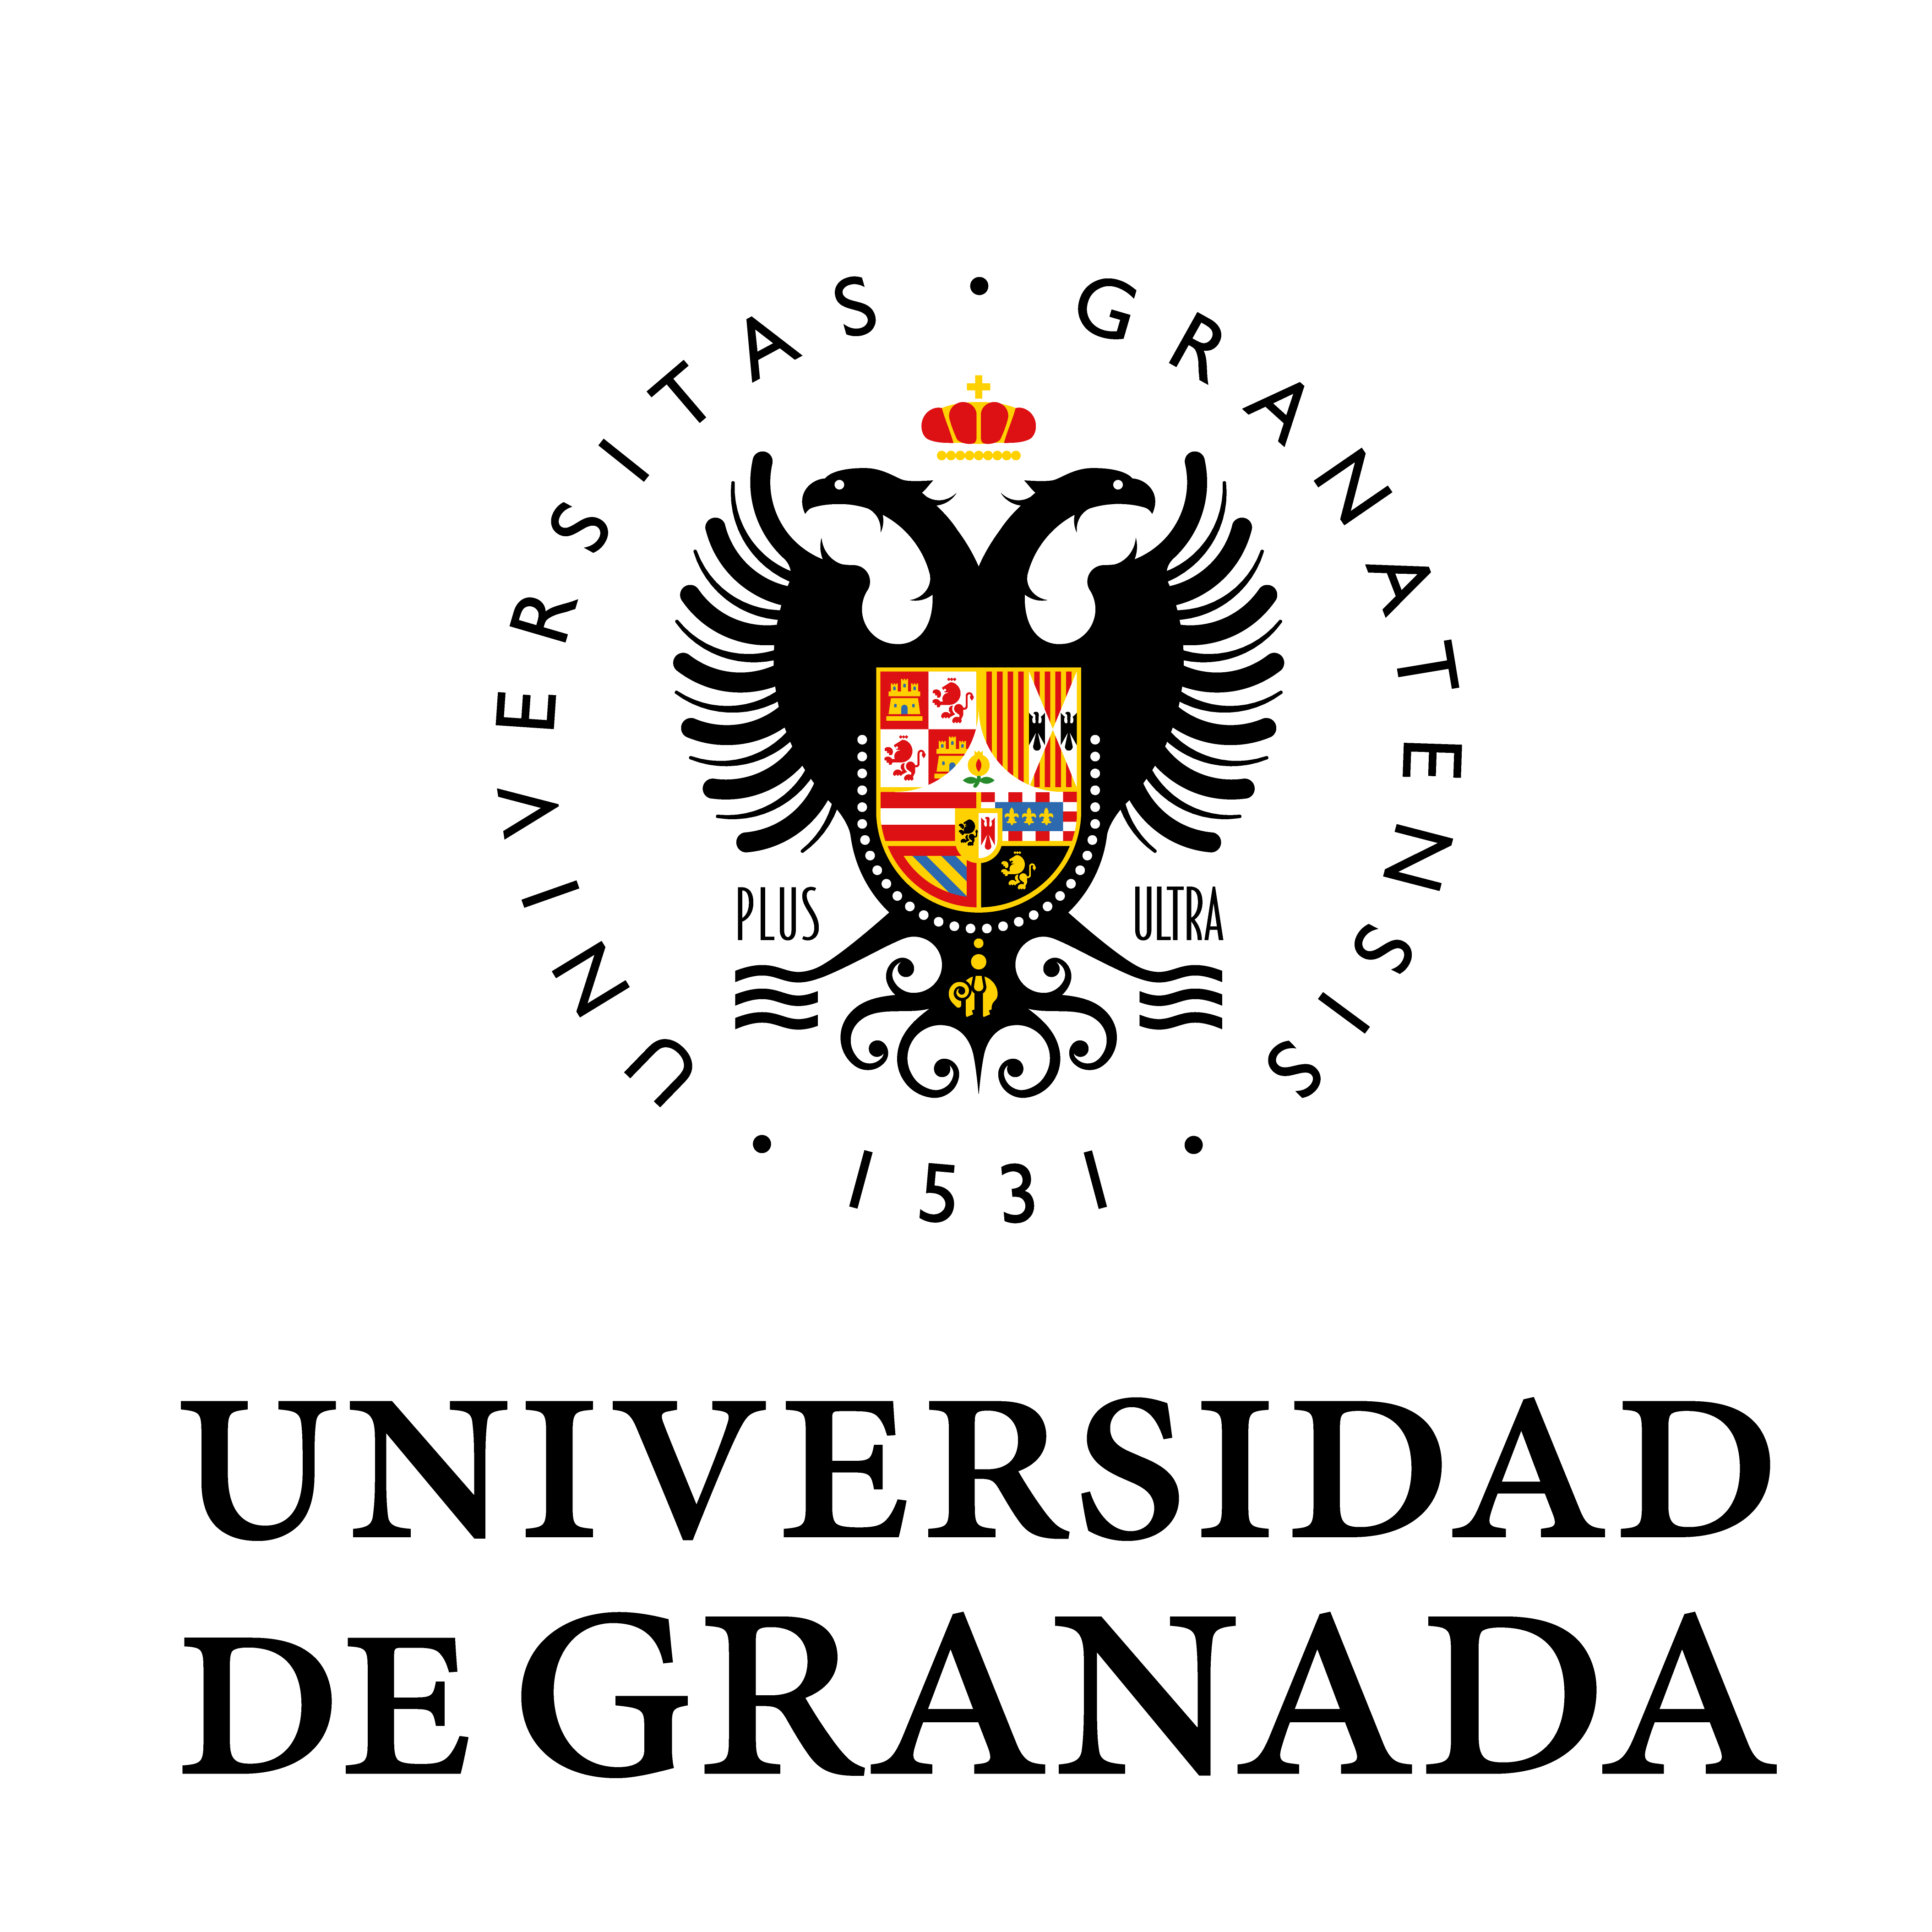
\includegraphics[scale = 0.50]{ugr.png}\\[0.7 cm]
    %\textsc{\LARGE Universidad de Granada}\\[2.0 cm]
    \textsc{\large 4º CSI 2020/21 - Grupo 2}\\[0.5 cm]
    \textsc{\large Grado en Ingeniería Informática}\\[0.5 cm]
    \rule{\linewidth}{0.2 mm} \\[0.2 cm]
    { \huge \bfseries \thetitle}\\
    \rule{\linewidth}{0.2 mm} \\[1 cm]

    \begin{minipage}{0.4\textwidth}
        \begin{flushleft} \large
            \emph{Autor:}\\
            \theauthor\\
			 \emph{DNI:}\\
            77021623-M
            \end{flushleft}
            \end{minipage}~
            \begin{minipage}{0.4\textwidth}
            \begin{flushright} \large
            \emph{Asignatura: \\
            Visión por Computador}   \\
            \emph{Correo:}\\
            advy99@correo.ugr.es
        \end{flushright}
    \end{minipage}\\[0.5cm]

    {\large \thedate}\\[0.5cm]
    %{\url{https://github.com/advy99/AA/}}
    {\doclicenseThis}

    \vfill

\end{titlepage}

%%%%%%%%%%%%%%%%%%%%%%%%%%%%%%%%%%%%%%%%%%%%%%%%%%%%%%%%%%%%%%%%%%%%%%%%%%%%%%%%%%%%%%%%%

\tableofcontents
\pagebreak

%%%%%%%%%%%%%%%%%%%%%%%%%%%%%%%%%%%%%%%%%%%%%%%%%%%%%%%%%%%%%%%%%%%%%%%%%%%%%%%%%%%%%%%%%


\section*{Introducción}

Para esta primera práctica trabajaremos los filtros de máscaras, con el objetivo de mostrar como usando técnicas de filtrado lineal es posible extraer información relevante de una imagen para su posterior interpretación.

En esta práctica también nos centraremos en comparar nuestra implementación propia con la implementación de la biblioteca OpenCV. Por este motivo, en todos los ejercicios utilizaré funciones implementadas en el fichero de Python entregado y en ciertos momentos utilizaré las funciones de filtros que nos ofrece OpenCV pero solo de forma comparativa.

En todo caso, en esta memoria me centraré en explicar que decisiones he tomado para el desarrollo de la práctica, así como parámetros escogidos, pero solo comentaré como funciona el código sin entrar en detalle, ya que junto a esta memoria se ha entregado un fichero con el código escrito en Python.

De cara al desarrollo de la práctica también se han utilizado funciones de la práctica 0, que al ya estar explicadas en su respectiva entrega no volveré a explicar.

\section{Ejercicio 1: Máscaras}

Este ejercicio trata sobre el cálculo de las máscaras Gaussianas que utilizaremos durante toda la práctica, la aplicación de dichas máscaras a una imagen en forma de una convolución 2D y el cálculo de máscaras normalizadas de la Laplaciana de la Gaussiana con nuestras propias máscaras.

Además de la implementación de todas estas máscaras, también realizaremos una comparación con las operaciones equivalentes de OpenCV.

\subsection{Máscaras discretas 1D}

De cara a obtener las distintas máscaras discretas he implementado tres funciones de Python:

\begin{enumerate}
	\item Función Gaussiana: Devuelve el valor de la función gaussiana en un punto dado, para un sigma dado.
	\item Función derivada de la Gaussiana: Devuelve el valor de la derivada de la gaussiana en un punto dado, para un sigma dado.
	\item Función segunda derivada de la Gaussiana: Devuelve el valor de la segunda derivada de la gaussiana en un punto dado, para un sigma dado.
\end{enumerate}


Para el cálculo de las distintas funciones simplemente he evaluado la función gaussiana, obviando la constante $c$ como hemos visto en teoría y como nos comentaron en prácticas:

\begin{figure}[H]
	\centering
	\[ f(x) = c \cdot e^{- \frac{x^2}{2\sigma^2}} \]
	\caption{Función gaussiana.}
	\label{f_gaussiana}
\end{figure}

\newpage

De cara a las funciones derivadas, simplemente he derivado la función gaussiana respecto de $x$:


\begin{figure}[H]
	\centering
	\[ \frac{\partial{f(x)}}{\partial{x}} = -\frac{e^{ -\frac{x^2}{2 \cdot \sigma^2} } \cdot x}{\sigma^2} \]
	\caption{Derivada de la función gaussiana.}
	\label{d_f_gaussiana}
\end{figure}

\begin{figure}[H]
	\centering
	\[ \frac{\partial{f(x)}}{\partial{x^2}} = -\frac{- x^2 + \sigma^2}{e^{ \frac{x^2}{2 \cdot \sigma^2} } \cdot \sigma^4} \]
	\caption{Segunda derivada de la función gaussiana.}
	\label{2d_f_gaussiana}
\end{figure}


Tras implementar estas funciones, que simplemente evaluavan una función matemática, he implementado la función \texttt{kernel\_gaussiano\_1d}, que obligatoriamente ha de recibir, o bien un sigma, o un tamaño para la máscara. Opcionalmenten puede recibir sobre que función se va a calcular la máscara, por defecto la función gaussiana, de forma que con esta función podamos calcular la máscara gaussiana, la máscara de la derivada de la gaussiana si le pasamos dicha función y la de la segunda derivada de la gaussiana si le pasamos esta última.

Como he comentado, esta función ha de recibir un sigma o un tamaño de máscara. Si recibe un sigma, calcula el tamaño de la máscara y devuelve la máscara evaluando los valores desde el entero menor a $\frac{tam\_mascara}{2}$ hasta $\frac{tam\_mascara}{2} + 1$ con el sigma dado. Si recibe el tamaño de máscara, calculará el sigma y devolverá la máscara calculada de la misma forma. Si no recibimos ni un sigma ni un tamaño de máscara, devolverá una máscara vacia.

Además, como vimos en teoría, si calculamos la máscara utilizando la función gaussiana antes de devolver el resultado lo noralizaremos dividiendo cada elemento de la máscara por la suma de todos, de forma que la máscara sume uno.

De cara a calcular el sigma o el tamaño de máscara seguiremos esta fórmula:


\begin{figure}[H]
	\centering
	\[ 2 \cdot 3 \cdot \sigma + 1 = T\]
	\caption{Calculo de sigma o del tamaño de máscara.}
	\label{sigma_t}
\end{figure}

Siendo T el tamaño de la máscara, podemos calcular dicho T o sigma en caso de que nos proporcionen T. Utilizamos esta fórmula ya que nos asegura que el tamaño de la máscara es al menos $3 \cdot \sigma$ como nos se nos recomendaba en teoría.

Otro detalle a observar es que si nos dan un sigma, el tamaño de la máscara es impar ya que, como también nos enseñaron en teoría, el uso de máscaras pares es problemático ya que no podemos centrar la máscara en un punto concreto de la imagen.

Tras realizar distintas ejecuciones de cara a probar el funcionamiento de esta función obtenemos lo siguiente:

\begin{lstlisting}
kernel_gaussiano_1d(sigma=1)
[0.00443305 0.05400558 0.24203623 0.39905028 0.24203623 0.05400558 0.00443305]

kernel_gaussiano_1d(func=derivada_f_gaussiana, tam_mascara=5)
[0.04999048442209038, 0.7304680515562869, -0.0, -0.7304680515562869, -0.04999048442209038]

kernel_gaussiano_1d(func=derivada_f_gaussiana, tam_mascara=7)
[0.033326989614726917, 0.2706705664732254, 0.6065306597126334, -0.0, -0.6065306597126334, -0.2706705664732254, -0.033326989614726917]
\end{lstlisting}


Podemos comprobar que obtenemos los resultados esperados, ya que el cálculo utilizando la función gaussiana hace que la máscara sume uno, y tanto la primera como segunda derivada suman cero, como era de esperar al haber estudiado estas funciones de forma teórica.


\subsection{Convolución gaussiana 2D}

Para desarrollar este ejercicio he creado la función \texttt{aplicar\_convolucion}, que recibe como parámetros la imagen, la máscara a aplicar de forma horizontal, la máscara a aplicar de forma vertical y el tipo de borde a añadir.

Este ultimo parámetro lo utilizaremos de cara a añadir bordes extra a la imagen, ya que si no aplicamos esta operación parte de los pixeles originales de las imágenes no se les aplicarían las máscaras, ya que el propio tamaño de máscara no permite centrarlas en dichos píxeles sin salir de la imágen.


Esta función sigue los siguientes pasos:

\begin{enumerate}
	\item Aplicar borde: Aplica un borde de tamaño $(len(mascara) - 1) / 2$ a la imagen utilizando la función de OpenCV \texttt{copyMakeBorder}.
	\item Crea una matriz rellena de ceros del tamaño de la imagen original (sin bordes), donde almacenaremos la imagen final.
	\item Recorre la imágen con borde (matriz) desde el tamaño del borde hasta el extremo de la imagen menos los bordes, de forma que pasamos por todos los píxeles de la imagen original. En este recorrido aplica la máscara horizontal, multiplicando la máscara por los pixeles de una misma fila, pero tantos como tamaño de máscara, centrando la máscara en el pixel actual que estamos recorriendo. De esta forma se aplica la máscara en el pixel que queremos y utilizando los bordes añadidos para los valores de la máscara que en principio quedarían fuera de la imagen original. Almacena el resultado en la matriz creada en el paso 2.
	\item Tras aplicar la máscara horizontal, volvemos a añadir los bordes a la imagen con la máscara aplicada, de cara a aplicar la máscara vertical.
	\item Repetimos el paso 3, pero al multiplicar la máscara, en lugar de mantener la fila y coger pixeles de distintas columnas, mantenemos la columna y escogemos un rango de píxeles en las filas para aplicar la máscara vertical. Almacenamos el resultado en la matriz creada en el paso 2.
	\item Normalizar la imagen final.
\end{enumerate}

Tras esta explicación de como funciona la función cabe mencionar distintos detalles de implementación.

Para empezar, vemos como aplico las máscaras de forma separada, y no como una convolución 2D. Esta decisión es tomada ya que el resultado obtenido es el mismo, sin embargo son necesarias menos operaciones para realizar el cálculo gracias a la separabilidad de las convoluciones 2D, haciendo más eficiente esta forma de aplicar las máscaras\cite{separabilidad_2D}.

Otro detalle es el hecho de añadir los bordes cada vez que aplico una convolución 1D. Aunque de esta forma es necesario mayor tiempo de cómputo al tener que volver a añadir bordes, se obtiene un mejor resultados en los bordes de la imagen resultante ya que si solamente se añaden bordes al inicio, al aplicar la segunda convolución usaría los bordes de la imagen original, que si utilizamos una técnica de replicado de bordes son distintos a los bordes de la imagen con una máscara aplicada, haciendo que al aplicar la segunda máscara en las zonas cercanas a los bordes el resultado no sea tan exacto.

Tambien mencionar que finalmente se normaliza la imagen en el rango [0-1] sin perdida de información ya que al aplicar la convolución la imagen no estará normalizada y dará problemas si intentamos visualizarla.

Finalmente, obtenemos este resultado aplicando una máscara de tamaño 9 y comparandola con GaussianBlur, con un tamaño de máscara 9 es el siguiente:


\begin{figure}[H]
  \centering
      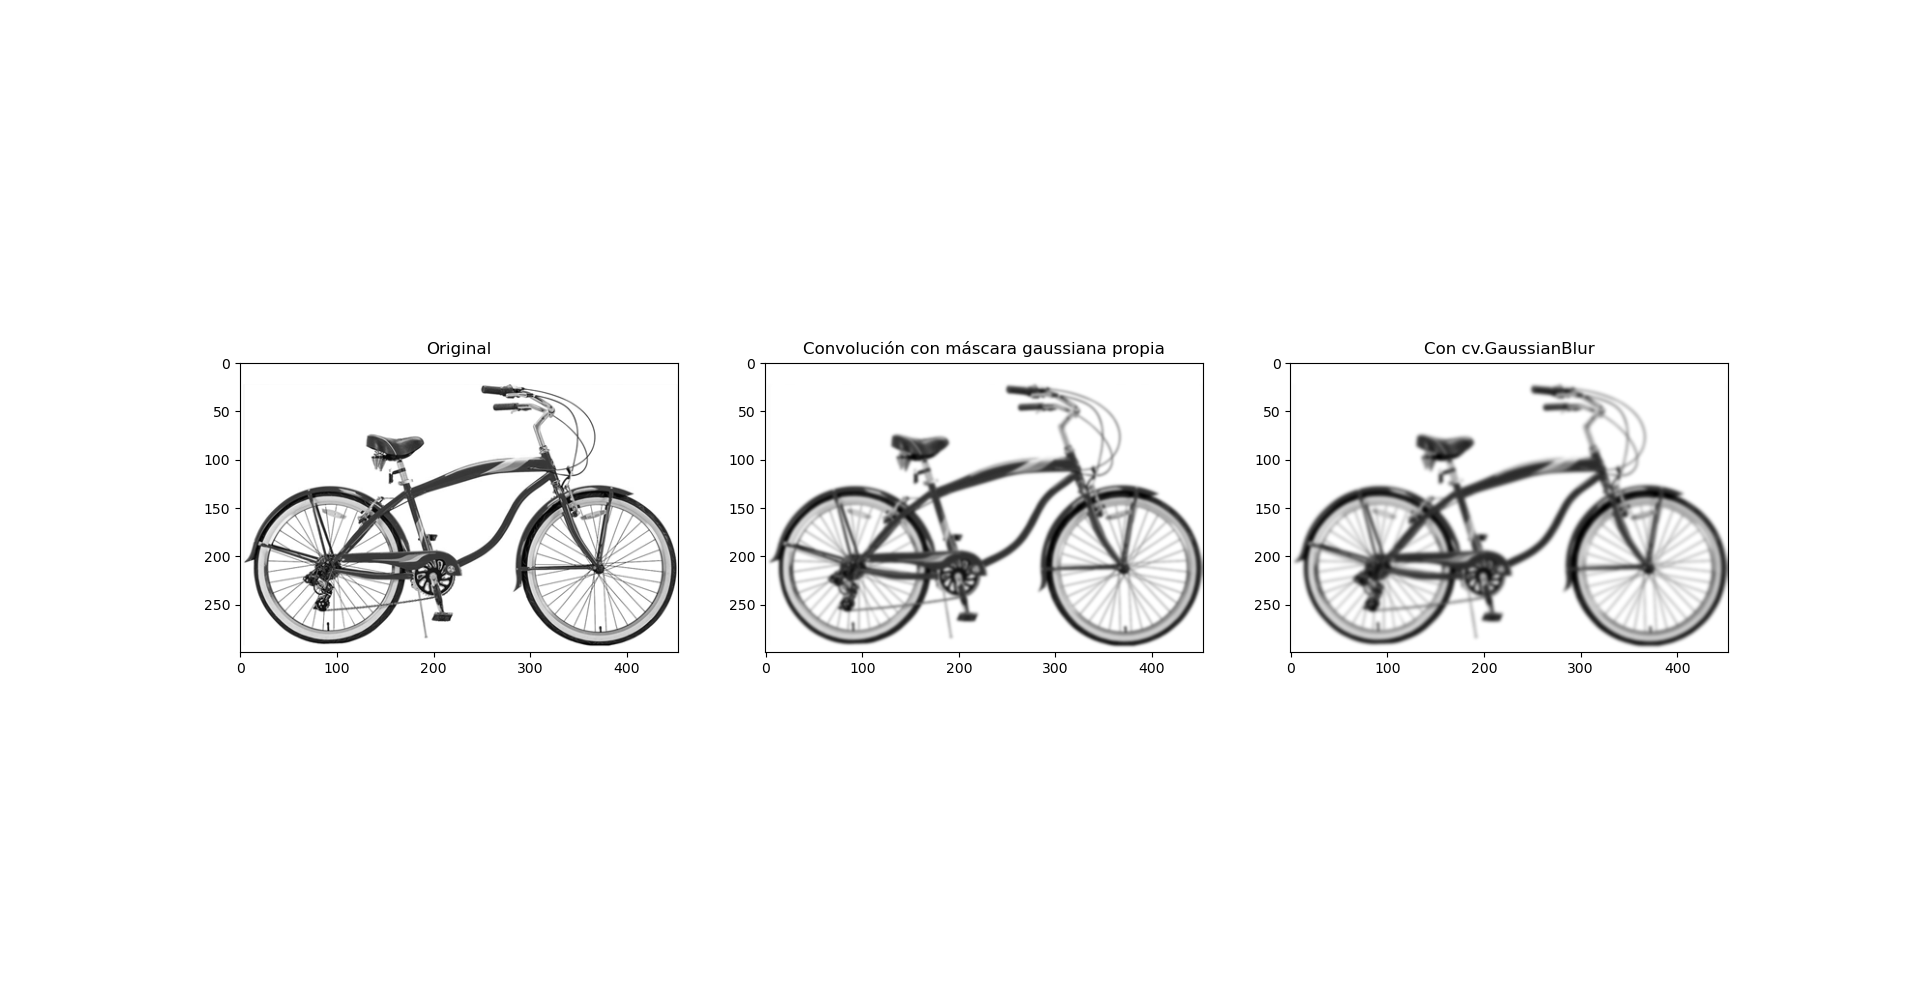
\includegraphics[width=\textwidth]{ejercicio1-b.png}
 		 \caption{Comparación entre implementación propia y GaussianBlur}
  		\label{fig:ej1b}

\end{figure}

Observamos como el resultado es similar, por lo que intuimos que la implementación tanto de la forma de obtener la máscara y la aplicación de la convolución es correcta.

\subsection{Comparación de máscaras 1D, implementación propia y OpenCV}

De cara a comparar mi implementación con las máscaras obtenidas con getDerivKernels de OpenCV, como nos pide el ejercicio, he generado las máscaras 1D con distintos tamaños de máscara y sigma y las he dibujado utilizando MatPlotLib:


\begin{figure}[H]
  \centering
	\begin{subfigure}[t]{0.4\textwidth}
		\centering
		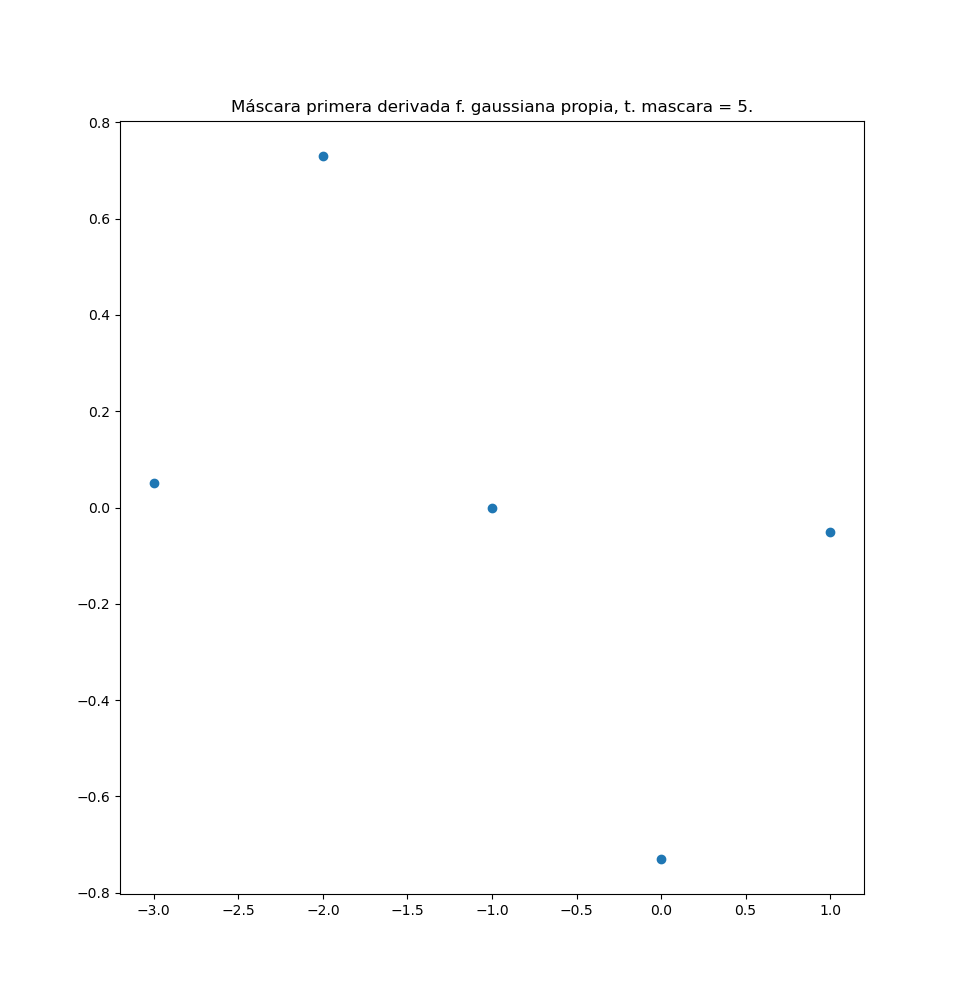
\includegraphics[width = \textwidth]{cmp-p5.png}
 		 \caption{Máscara primera derivada propia, t. máscara 5}
	\end{subfigure}
	\hspace{1cm}
	\begin{subfigure}[t]{0.4\textwidth}
		\centering
		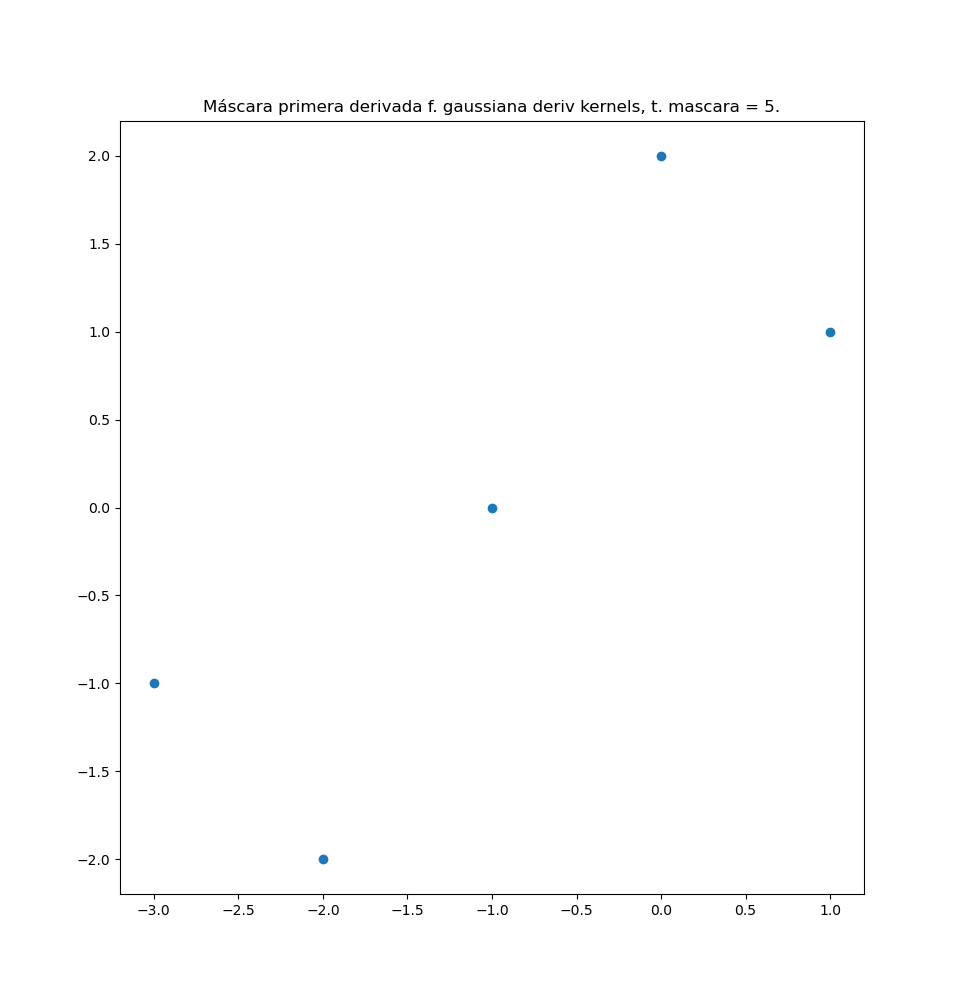
\includegraphics[width = \textwidth]{cmp-cv5.png}
 		 \caption{Máscara primera derivada OpenCV, t. máscara 5}
	\end{subfigure}
	\caption{Comparación primera derivada, tamaño de máscara 5}
  	\label{fig:ej1c5}
\end{figure}


\begin{figure}[H]
  \centering
	\begin{subfigure}[t]{0.4\textwidth}
		\centering
		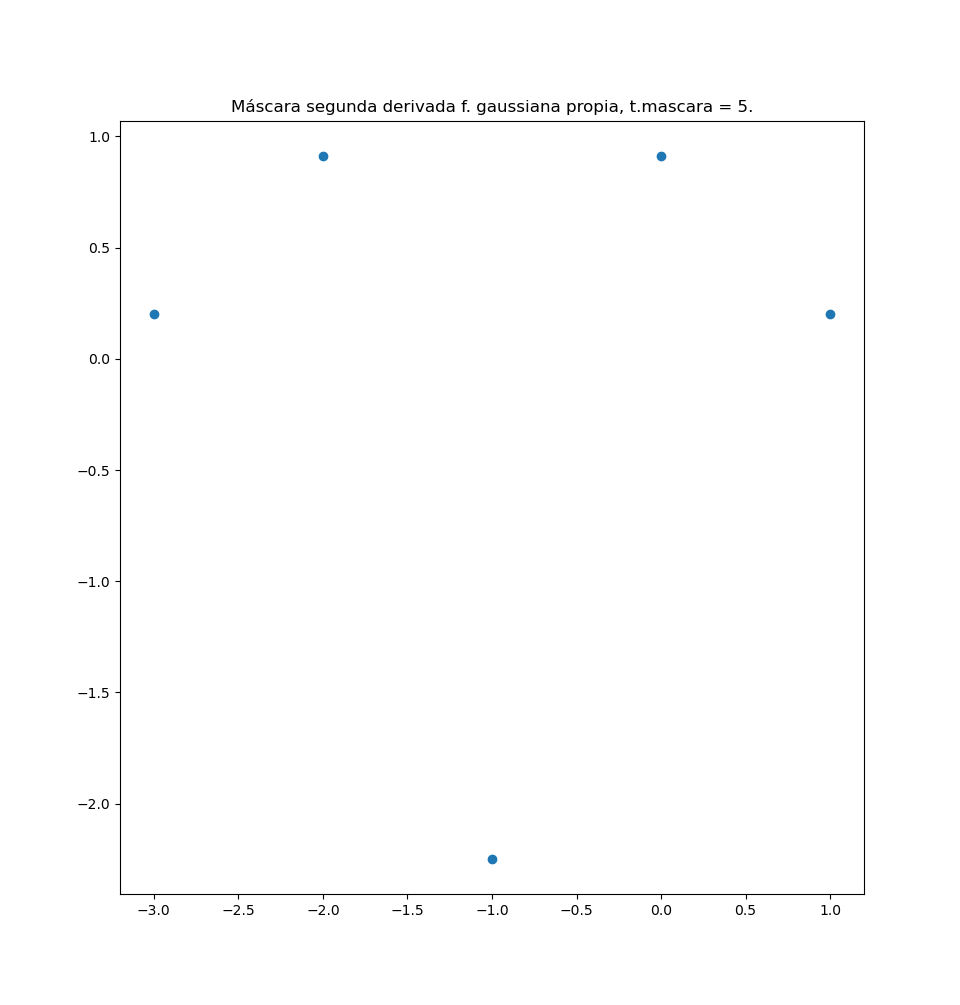
\includegraphics[width = \textwidth]{cmp-2p5.png}
 		 \caption{Máscara segunda derivada propia, t. máscara 5}
	\end{subfigure}
	\hspace{1cm}
	\begin{subfigure}[t]{0.4\textwidth}
		\centering
		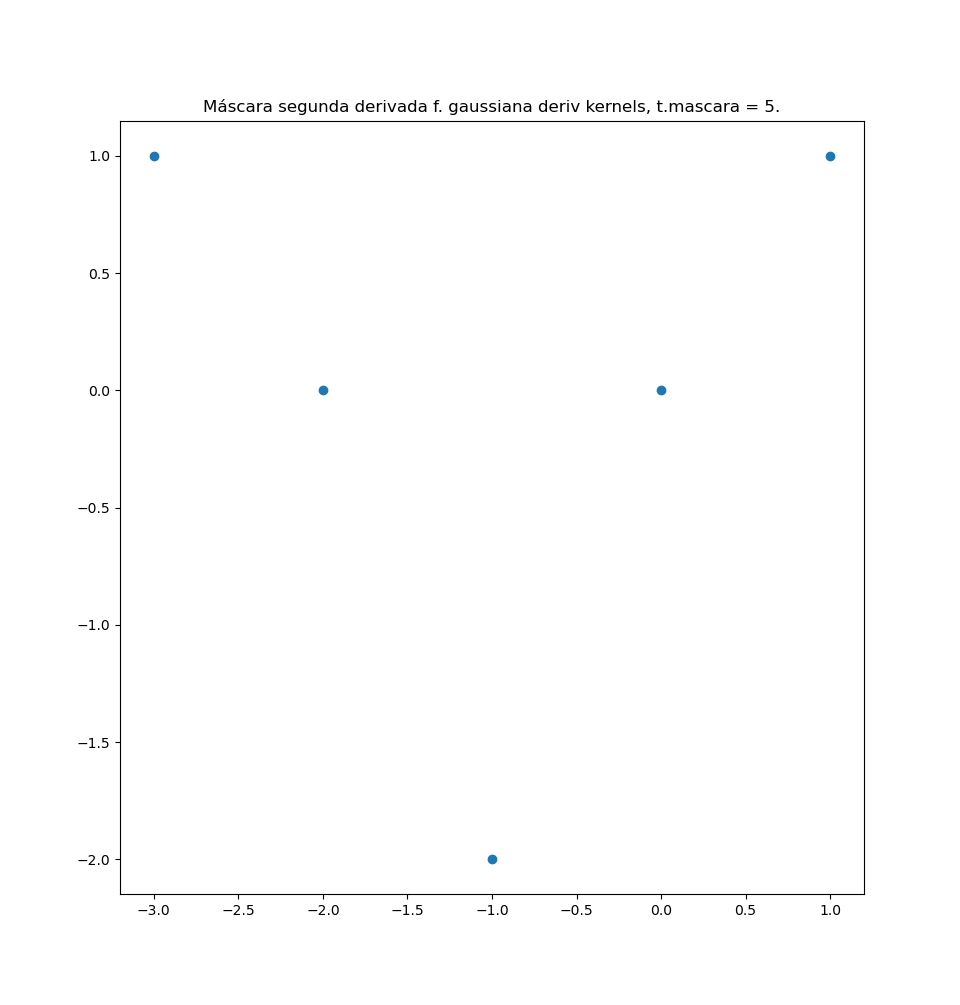
\includegraphics[width = \textwidth]{cmp-2cv5.png}
 		 \caption{Máscara segunda derivada OpenCV, t. máscara 5}
	\end{subfigure}
	\caption{Comparación segunda derivada, tamaño de máscara 5}

  	\label{fig:ej1c5}
\end{figure}


\begin{figure}[H]
  \centering
	\begin{subfigure}[t]{0.4\textwidth}
		\centering
		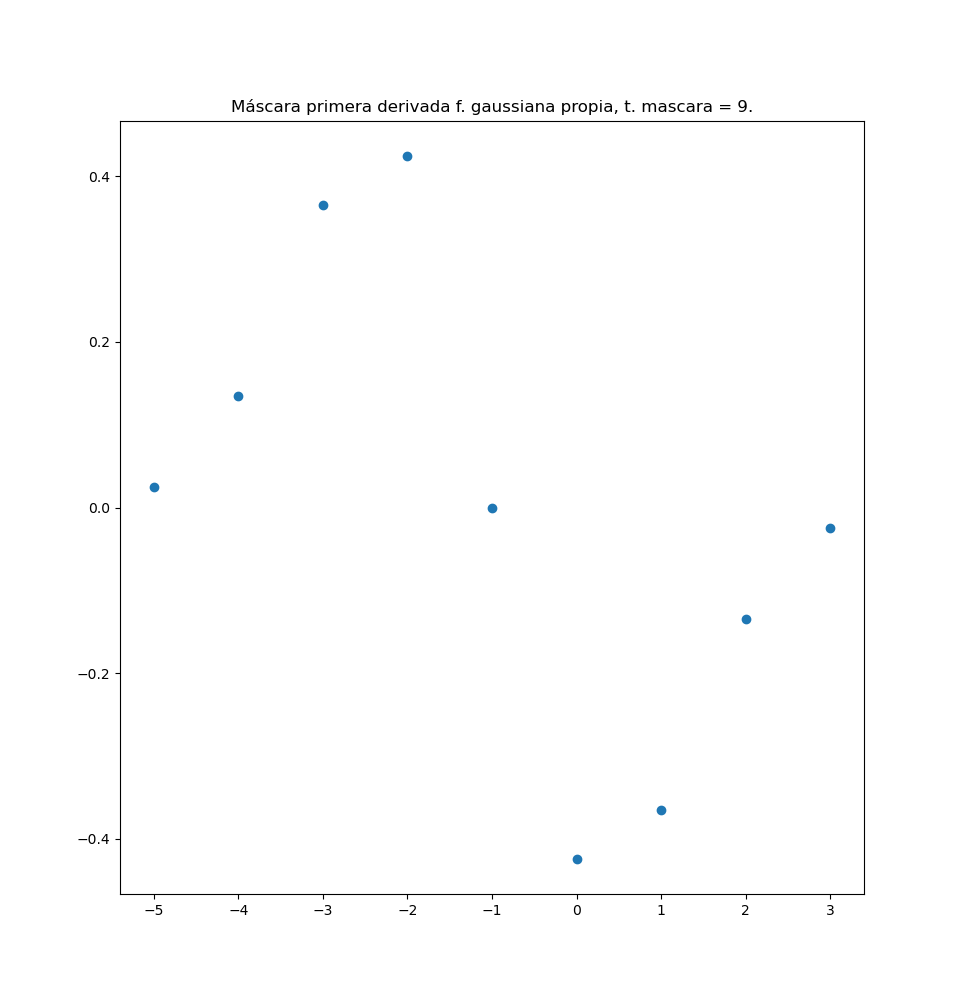
\includegraphics[width = \textwidth]{cmp-p9.png}
 		 \caption{Máscara primera derivada propia, t. máscara 9}
	\end{subfigure}
	\hspace{1cm}
	\begin{subfigure}[t]{0.4\textwidth}
		\centering
		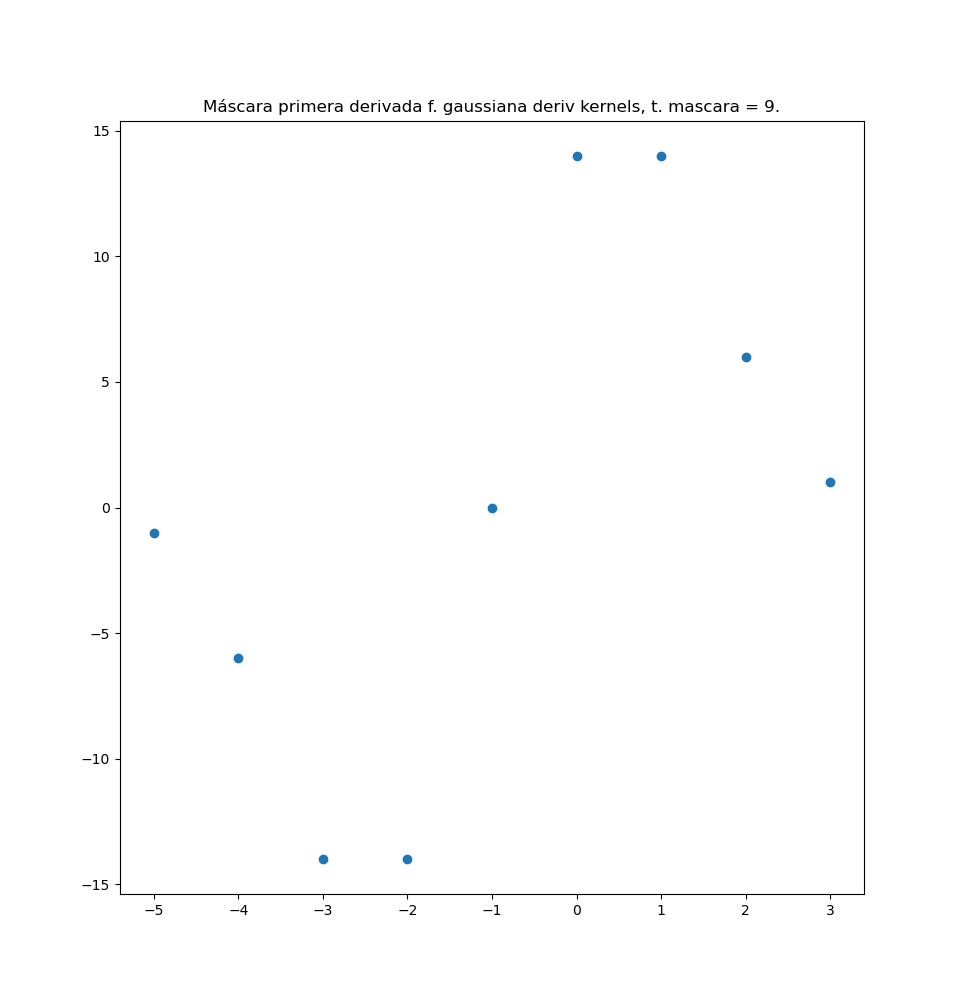
\includegraphics[width = \textwidth]{cmp-cv9.png}
 		 \caption{Máscara primera derivada OpenCV, t. máscara 9}
	\end{subfigure}
	\caption{Comparación primera derivada, tamaño de máscara 9}
  	\label{fig:ej1c5}
\end{figure}


\begin{figure}[H]
  \centering
	\begin{subfigure}[t]{0.4\textwidth}
		\centering
		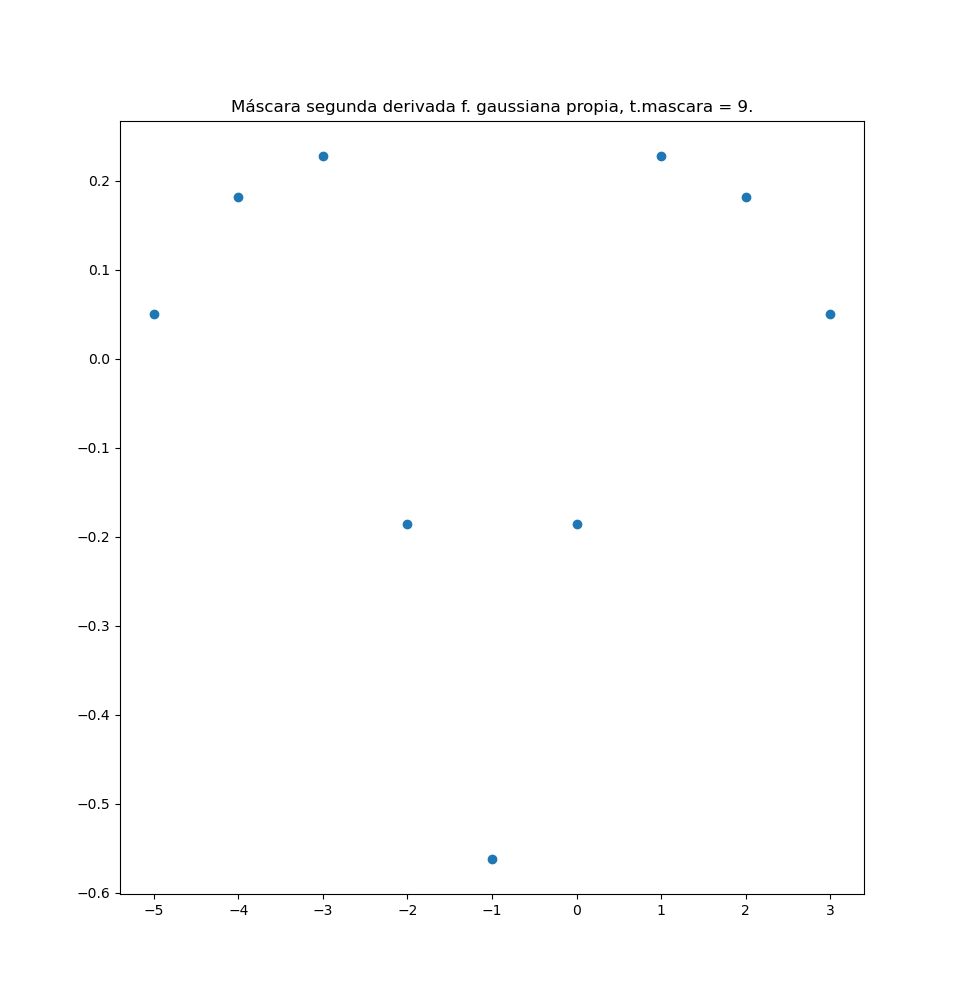
\includegraphics[width = \textwidth]{cmp-2p9.png}
 		 \caption{Máscara segunda derivada propia, t. máscara 9}
	\end{subfigure}
	\hspace{1cm}
	\begin{subfigure}[t]{0.4\textwidth}
		\centering
		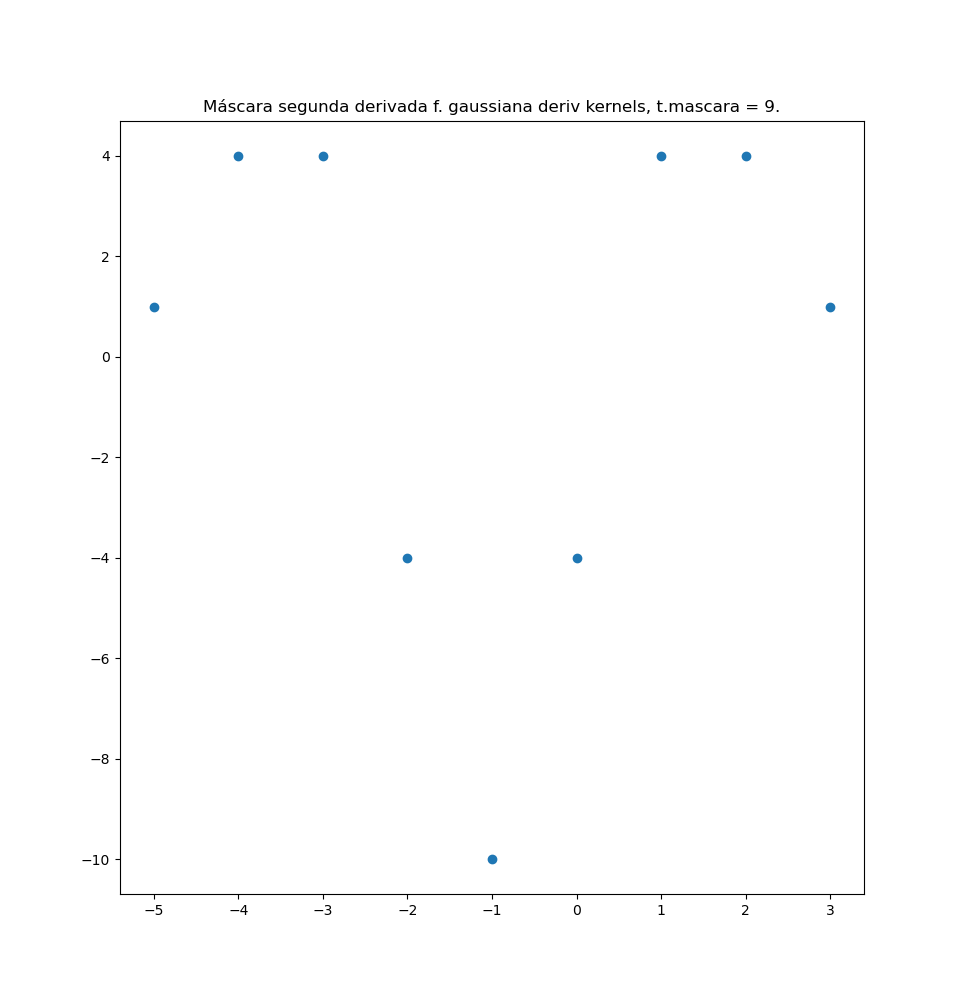
\includegraphics[width = \textwidth]{cmp-2cv9.png}
 		 \caption{Máscara segunda derivada OpenCV, t. máscara 9}
	\end{subfigure}
	\caption{Comparación segunda derivada, tamaño de máscara 9}

  	\label{fig:ej1c5}
\end{figure}


\begin{figure}[H]
  \centering
	\begin{subfigure}[t]{0.4\textwidth}
		\centering
		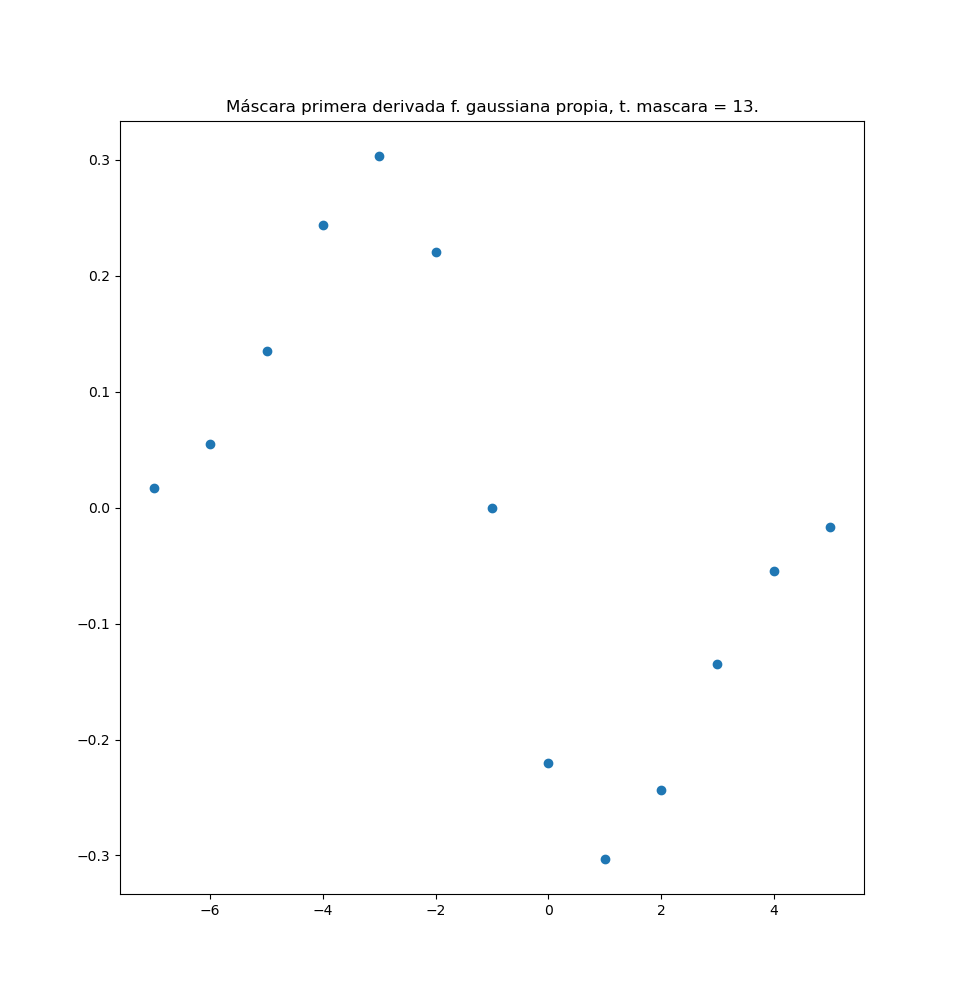
\includegraphics[width = \textwidth]{cmp-p13.png}
 		 \caption{Máscara primera derivada propia, t. máscara 13}
	\end{subfigure}
	\hspace{1cm}
	\begin{subfigure}[t]{0.4\textwidth}
		\centering
		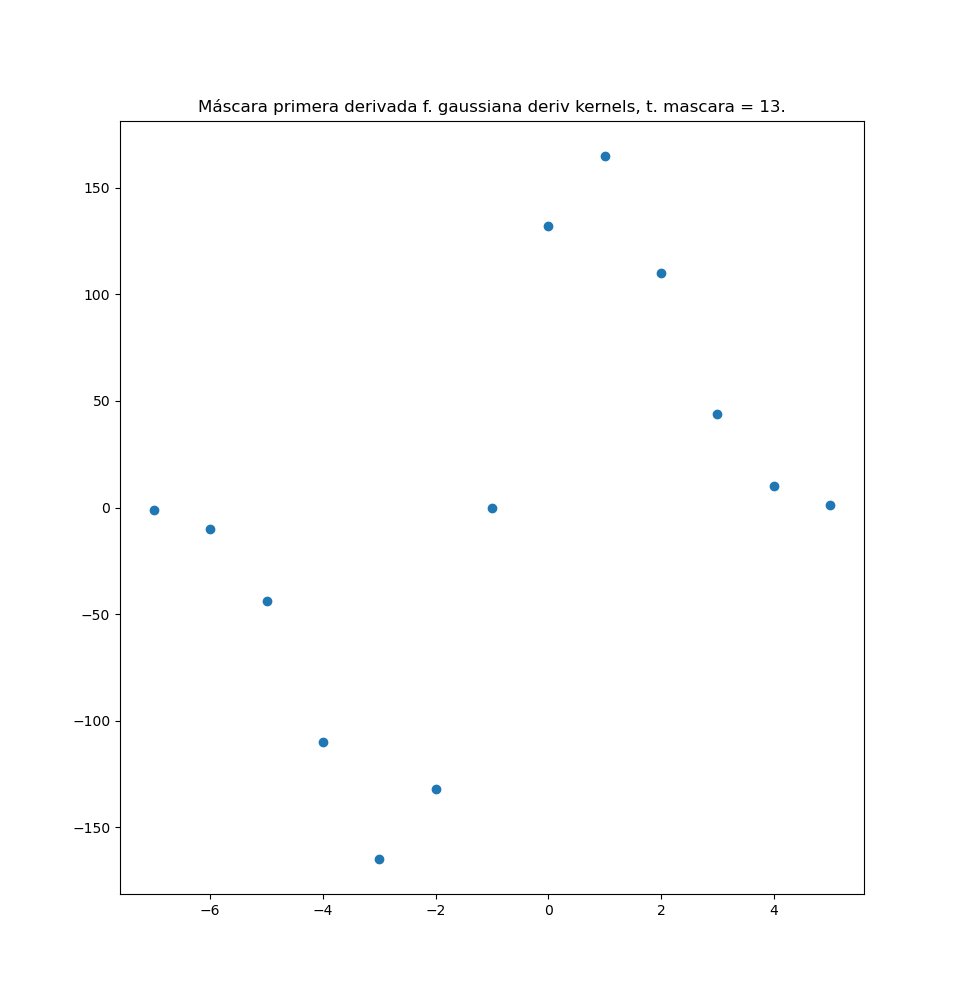
\includegraphics[width = \textwidth]{cmp-cv13.png}
 		 \caption{Máscara primera derivada OpenCV, t. máscara 13}
	\end{subfigure}
	\caption{Comparación primera derivada, tamaño de máscara 13}
  	\label{fig:ej1c5}
\end{figure}


\begin{figure}[H]
  \centering
	\begin{subfigure}[t]{0.4\textwidth}
		\centering
		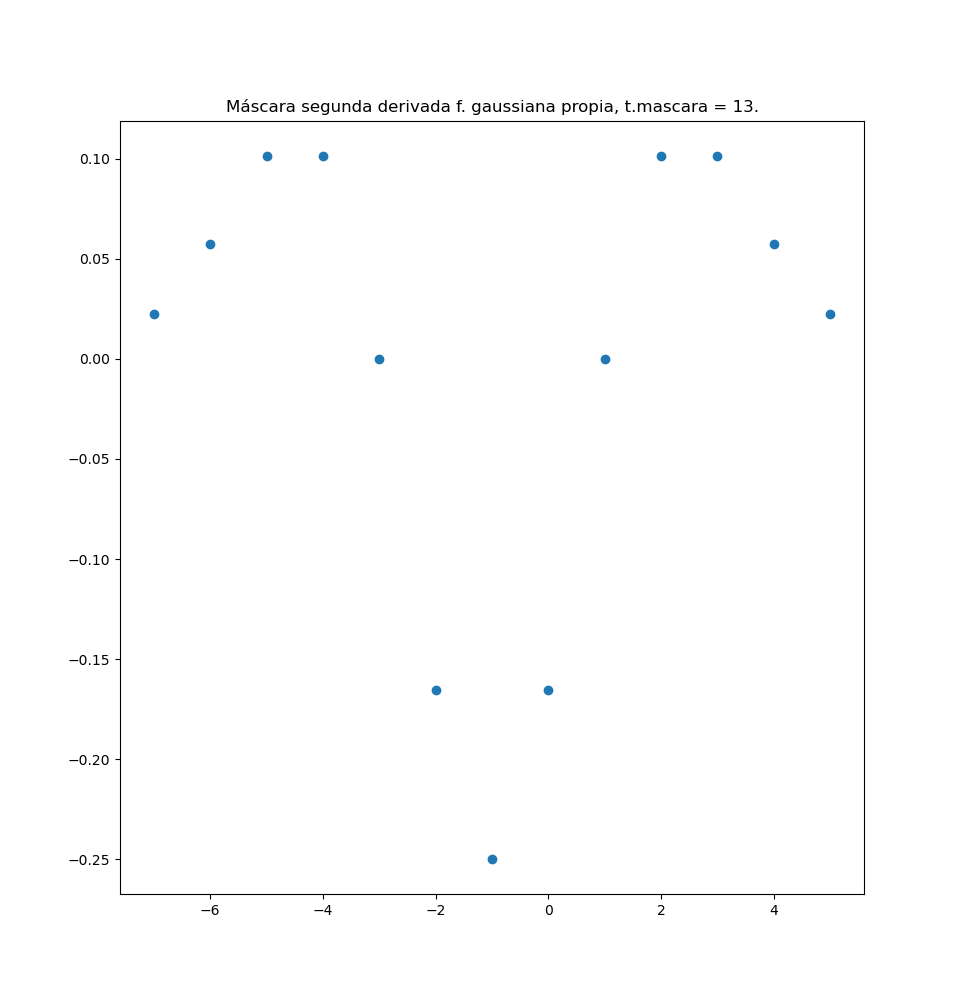
\includegraphics[width = \textwidth]{cmp-2p13.png}
 		 \caption{Máscara segunda derivada propia, t. máscara 13}
	\end{subfigure}
	\hspace{1cm}
	\begin{subfigure}[t]{0.4\textwidth}
		\centering
		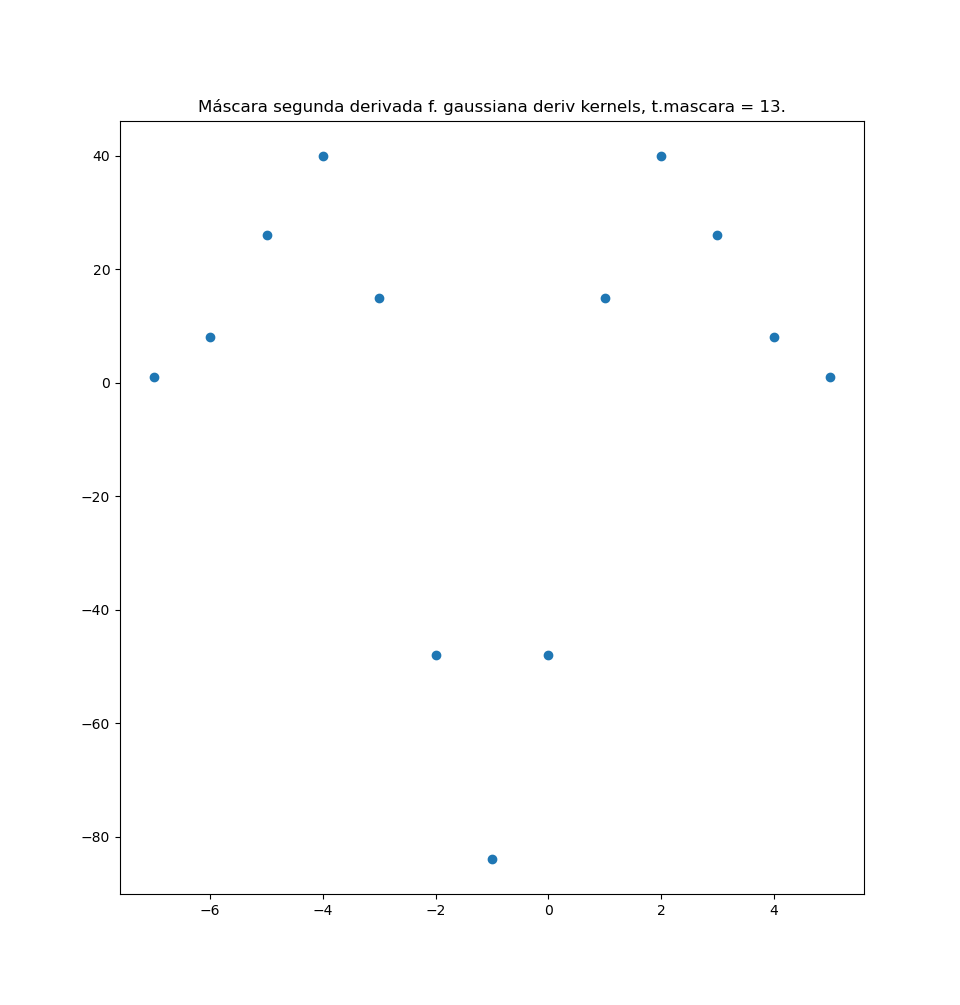
\includegraphics[width = \textwidth]{cmp-2cv13.png}
 		 \caption{Máscara segunda derivada OpenCV, t. máscara 13}
	\end{subfigure}
	\caption{Comparación segunda derivada, tamaño de máscara 13}

  	\label{fig:ej1c5}
\end{figure}



\begin{figure}[H]
  \centering
	\begin{subfigure}[t]{0.4\textwidth}
		\centering
		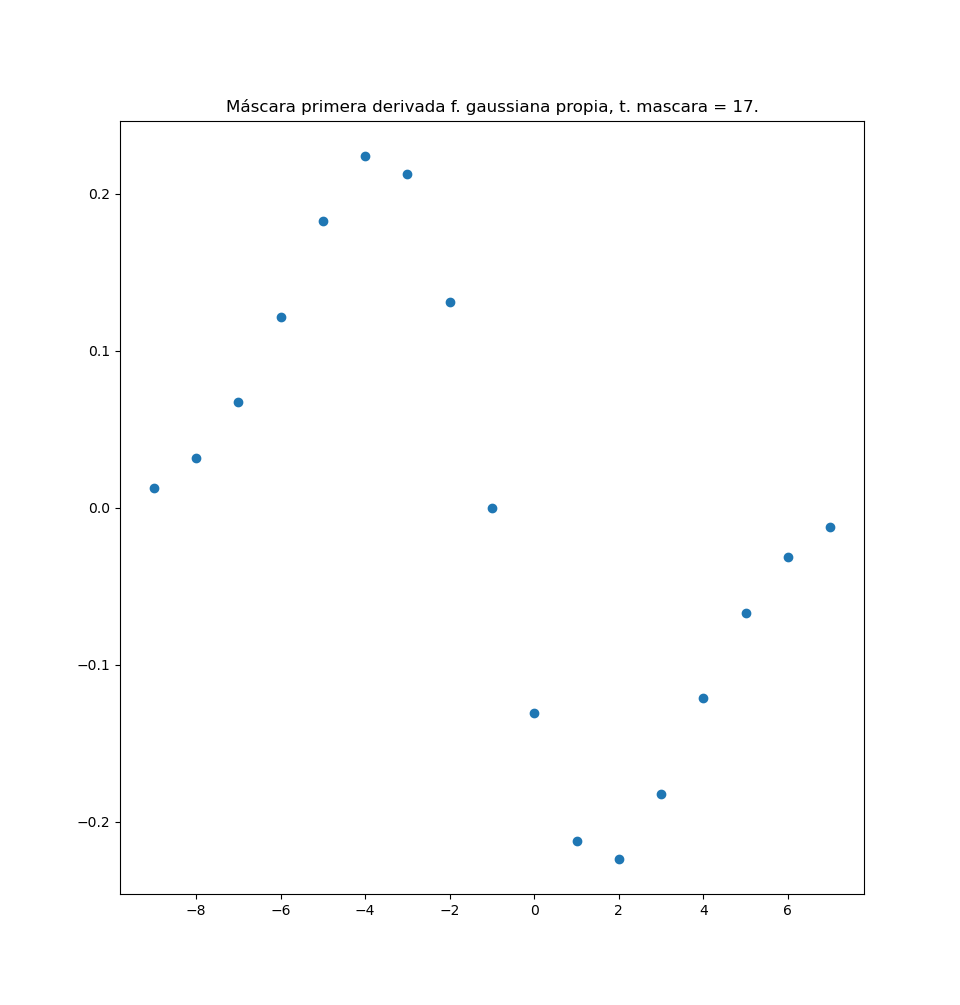
\includegraphics[width = \textwidth]{cmp-p17.png}
 		 \caption{Máscara primera derivada propia, t. máscara 17}
	\end{subfigure}
	\hspace{1cm}
	\begin{subfigure}[t]{0.4\textwidth}
		\centering
		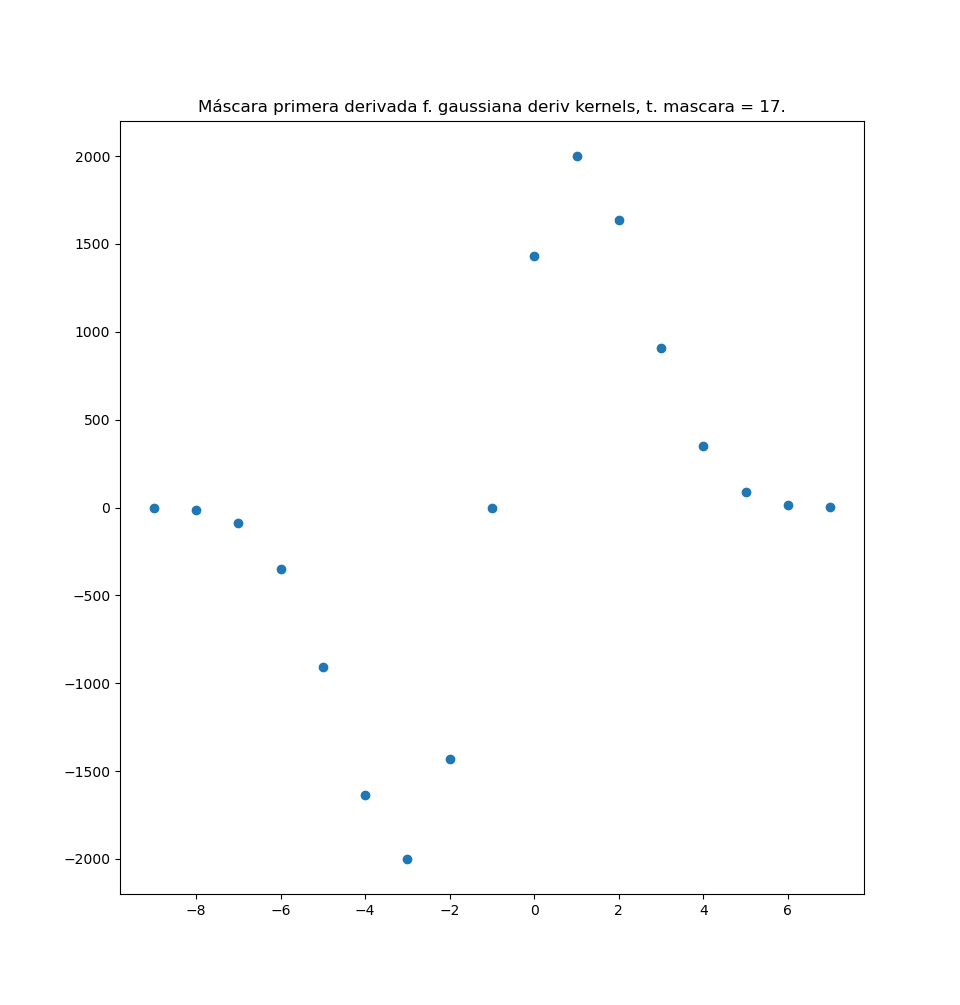
\includegraphics[width = \textwidth]{cmp-cv17.png}
 		 \caption{Máscara primera derivada OpenCV, t. máscara 17}
	\end{subfigure}
	\caption{Comparación primera derivada, tamaño de máscara 17}
  	\label{fig:ej1c5}
\end{figure}


\begin{figure}[H]
  \centering
	\begin{subfigure}[t]{0.4\textwidth}
		\centering
		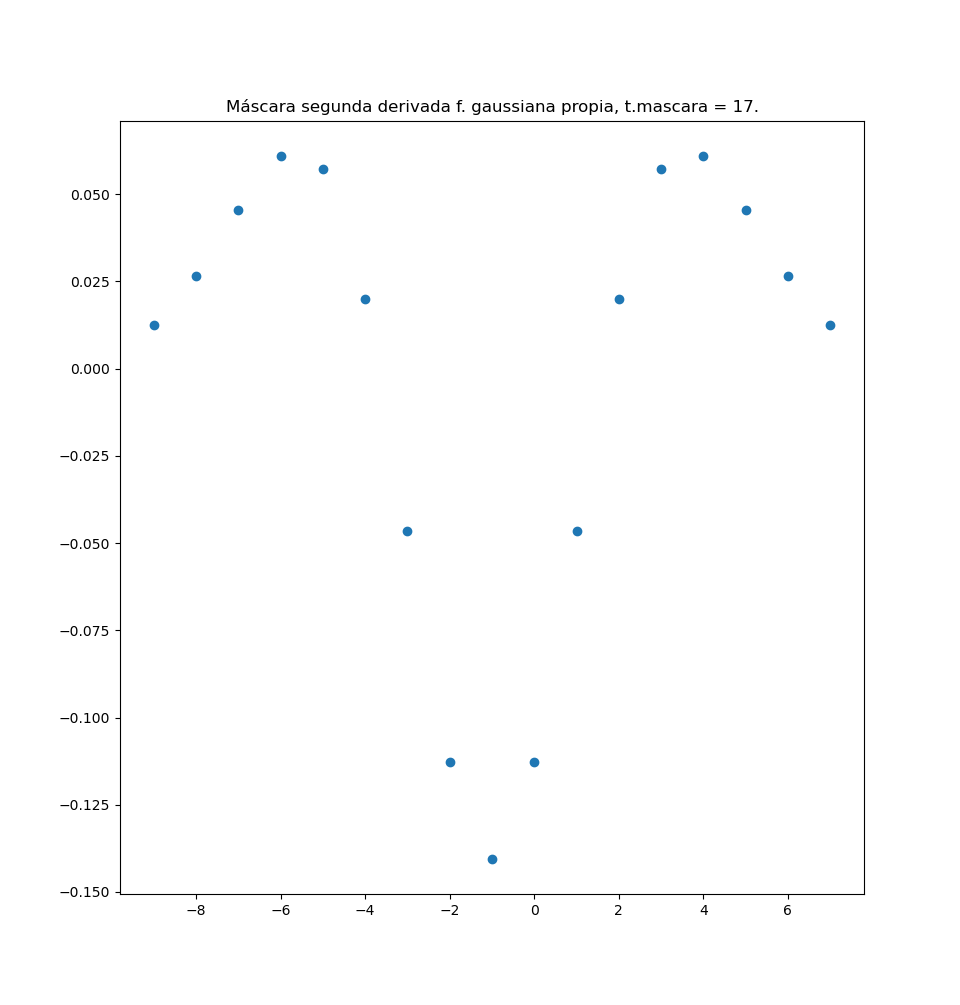
\includegraphics[width = \textwidth]{cmp-2p17.png}
 		 \caption{Máscara segunda derivada propia, t. máscara 17}
	\end{subfigure}
	\hspace{1cm}
	\begin{subfigure}[t]{0.4\textwidth}
		\centering
		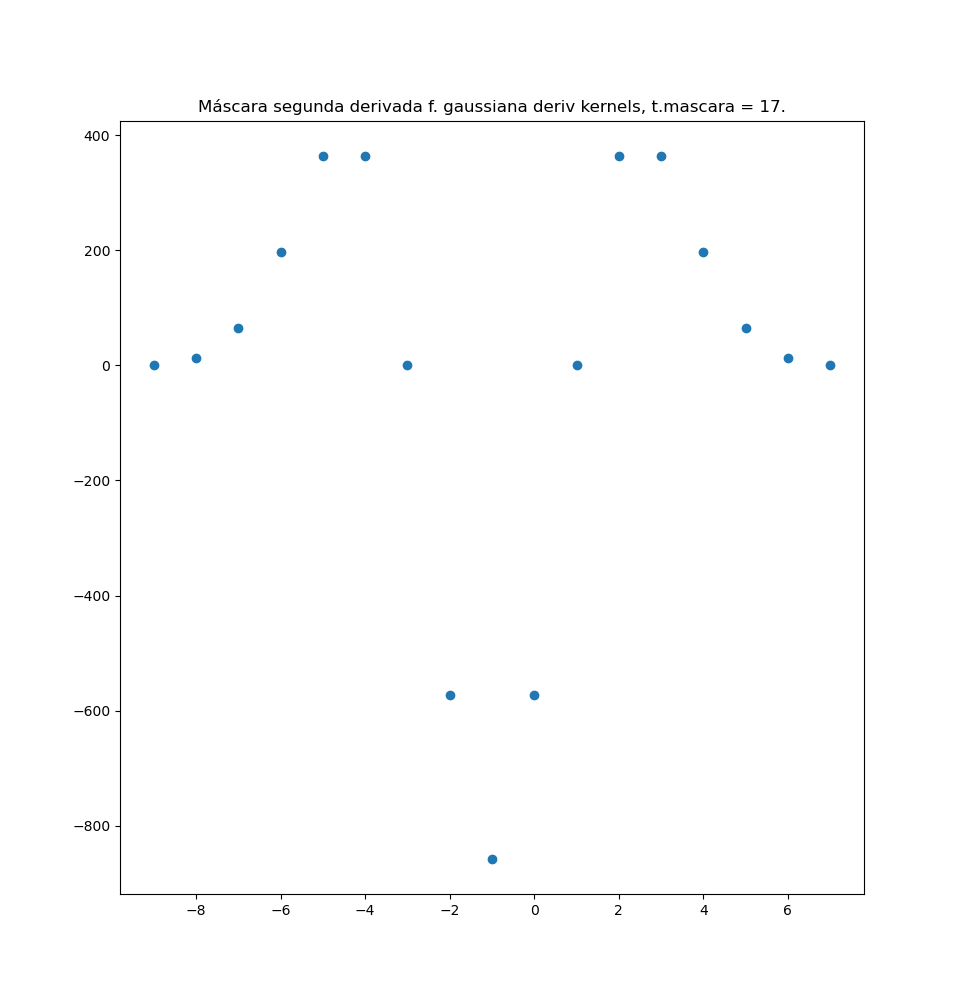
\includegraphics[width = \textwidth]{cmp-2cv17.png}
 		 \caption{Máscara segunda derivada OpenCV, t. máscara 17}
	\end{subfigure}
	\caption{Comparación segunda derivada, tamaño de máscara 17}

  	\label{fig:ej1c5}
\end{figure}


\begin{figure}[H]
  \centering
	\begin{subfigure}[t]{0.4\textwidth}
		\centering
		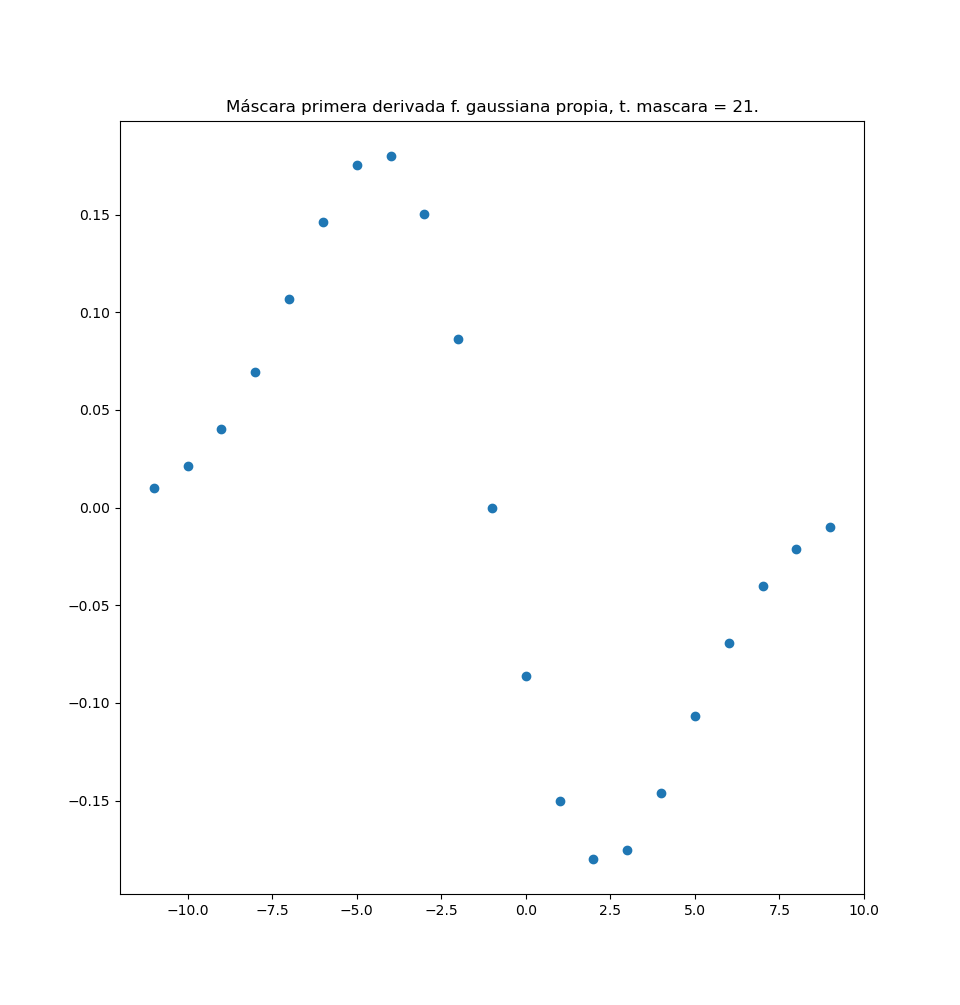
\includegraphics[width = \textwidth]{cmp-p21.png}
 		 \caption{Máscara primera derivada propia, t. máscara 21}
	\end{subfigure}
	\hspace{1cm}
	\begin{subfigure}[t]{0.4\textwidth}
		\centering
		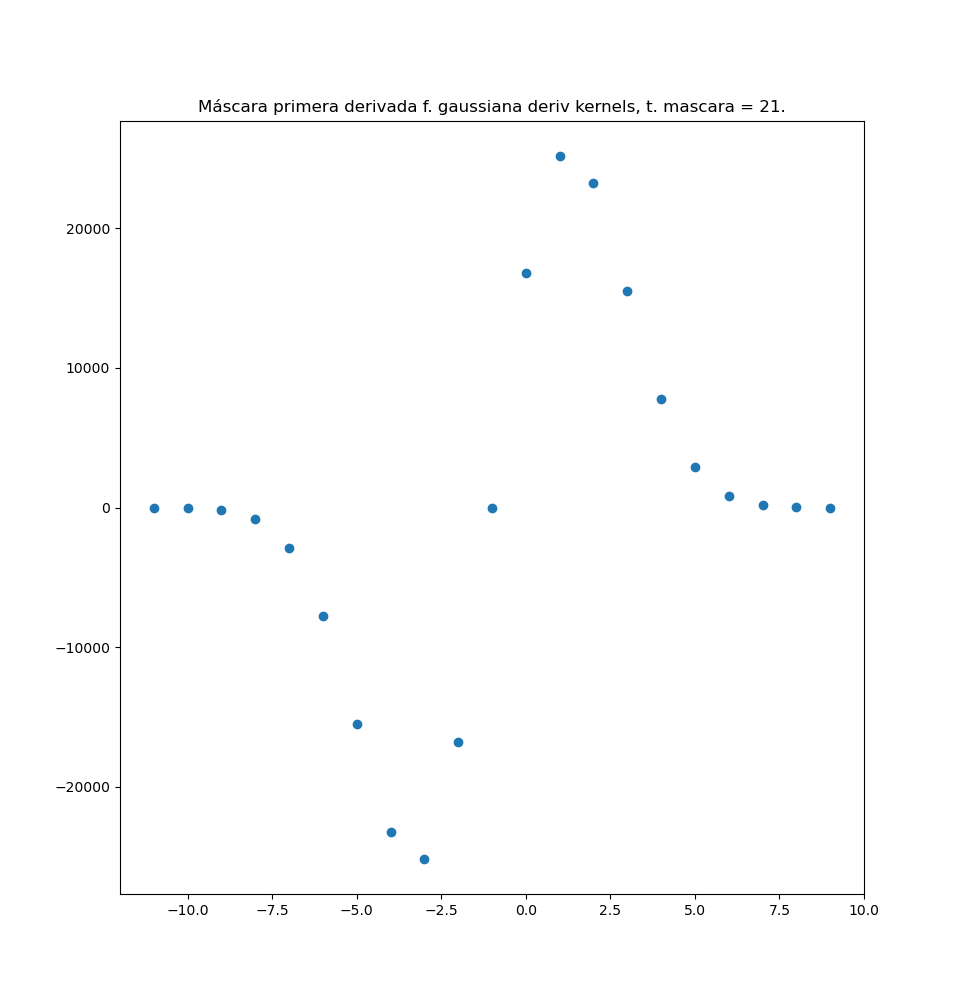
\includegraphics[width = \textwidth]{cmp-cv21.png}
 		 \caption{Máscara primera derivada OpenCV, t. máscara 21}
	\end{subfigure}
	\caption{Comparación primera derivada, tamaño de máscara 21}
  	\label{fig:ej1c5}
\end{figure}


\begin{figure}[H]
  \centering
	\begin{subfigure}[t]{0.4\textwidth}
		\centering
		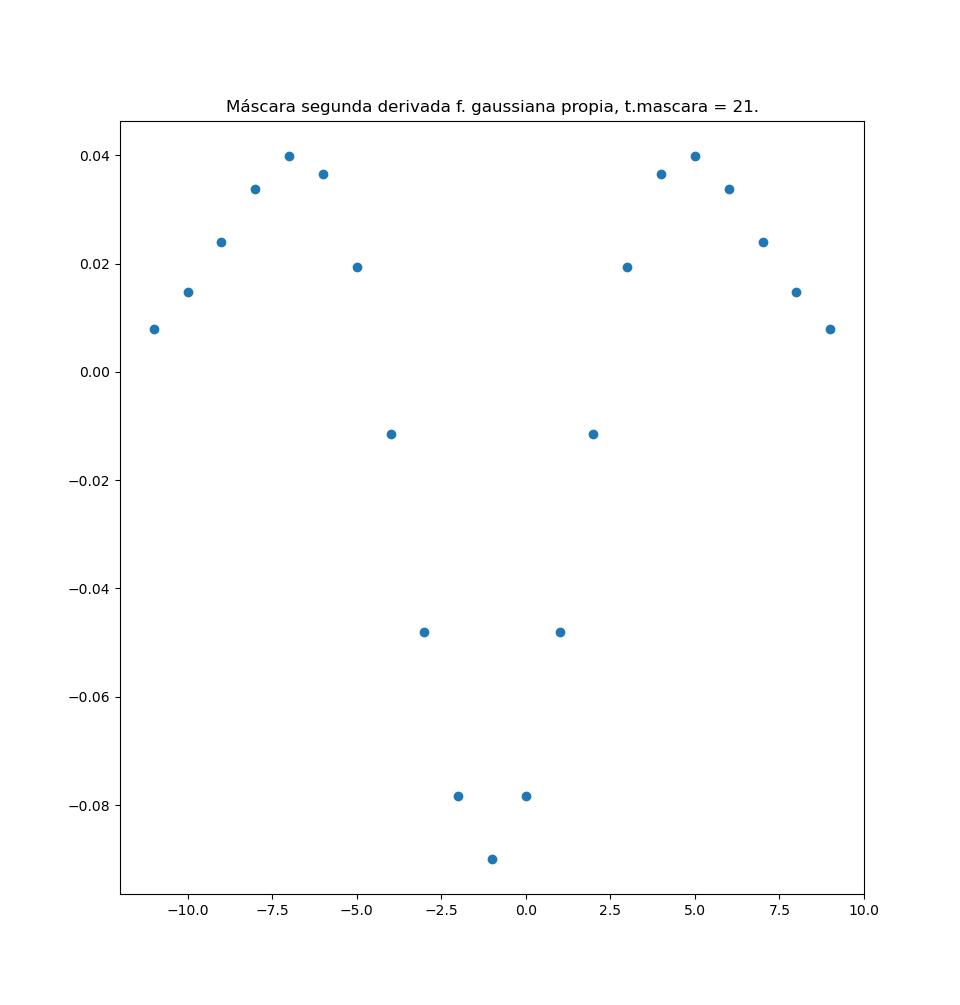
\includegraphics[width = \textwidth]{cmp-2p21.png}
 		 \caption{Máscara segunda derivada propia, t. máscara 21}
	\end{subfigure}
	\hspace{1cm}
	\begin{subfigure}[t]{0.4\textwidth}
		\centering
		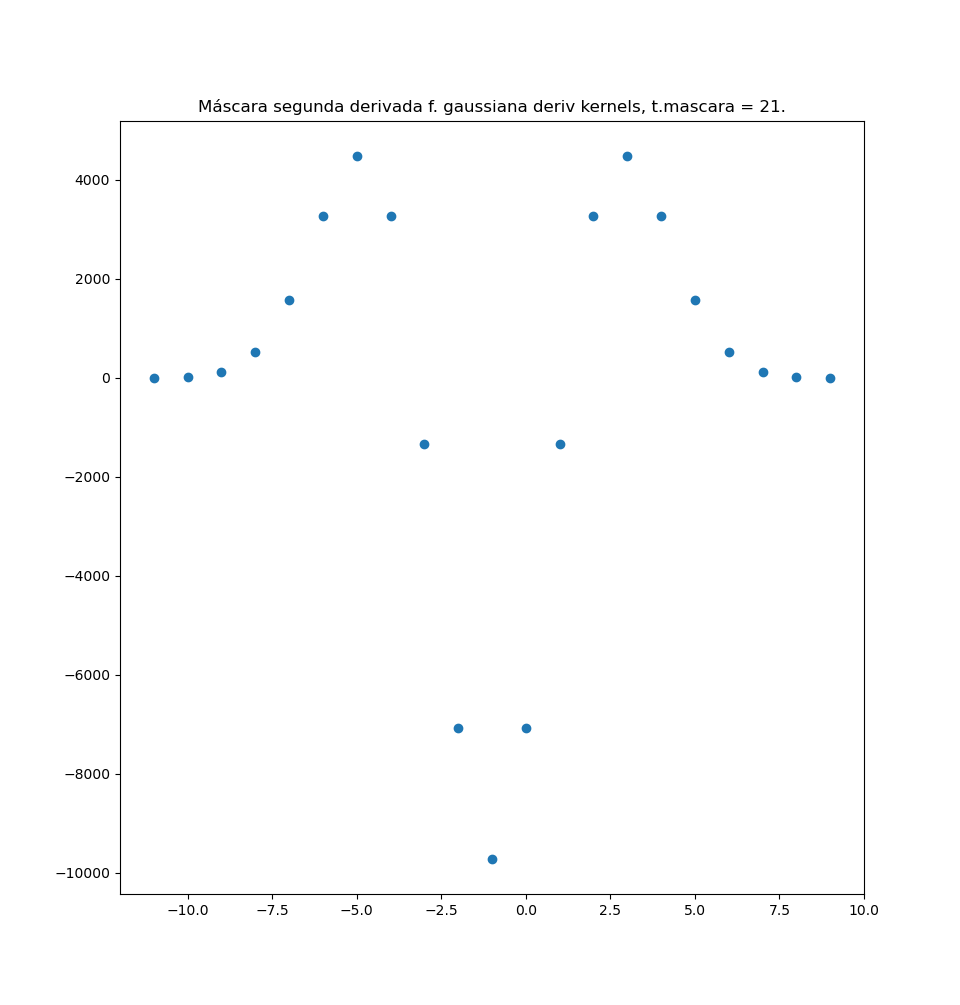
\includegraphics[width = \textwidth]{cmp-2cv21.png}
 		 \caption{Máscara segunda derivada OpenCV, t. máscara 21}
	\end{subfigure}
	\caption{Comparación segunda derivada, tamaño de máscara 21}

  	\label{fig:ej1c5}
\end{figure}


Tras observar todas las máscaras podemos observar dos grandes diferencias:

\begin{enumerate}
	\item Las máscaras de la primera derivada están invertidas con respecto al eje X. En nuestra implementación propia a la izquierda del 0 hay un máximo y a la derecha un mínimo, mientras que las máscaras obtenidas con getDerivKernels es al contrario.
	\item Cuanto mayor es el tamaño de la máscara, menor es el rango de valores en nuestras máscaras y mayor en las máscaras generadas por getDerivKernels.
\end{enumerate}

La primera diferencia es irrelevante respecto al funcionamiento ya que las máscaras son simetricas, luego la suma de los valores es igualmente cero.

Con respecto a la segunda diferencia, y en general todas las diferencias que podamos encontrar, es debidas a que mientras nosotros calculamos las máscaras de forma exacta, OpenCV hace una aproximación de las derivadas de la gaussiana utilizando los operadores de Sobel y Scharr\cite{getDerivKernelsCV}, haciendo que en realidad las máscaras obtenidas por OpenCV, aunque el tiempo de cómputo es menor, no son tan exactas.

Por último, a pesar de estas diferencias vemos que los resultados son equivalentes:


\begin{figure}[H]
  \centering
      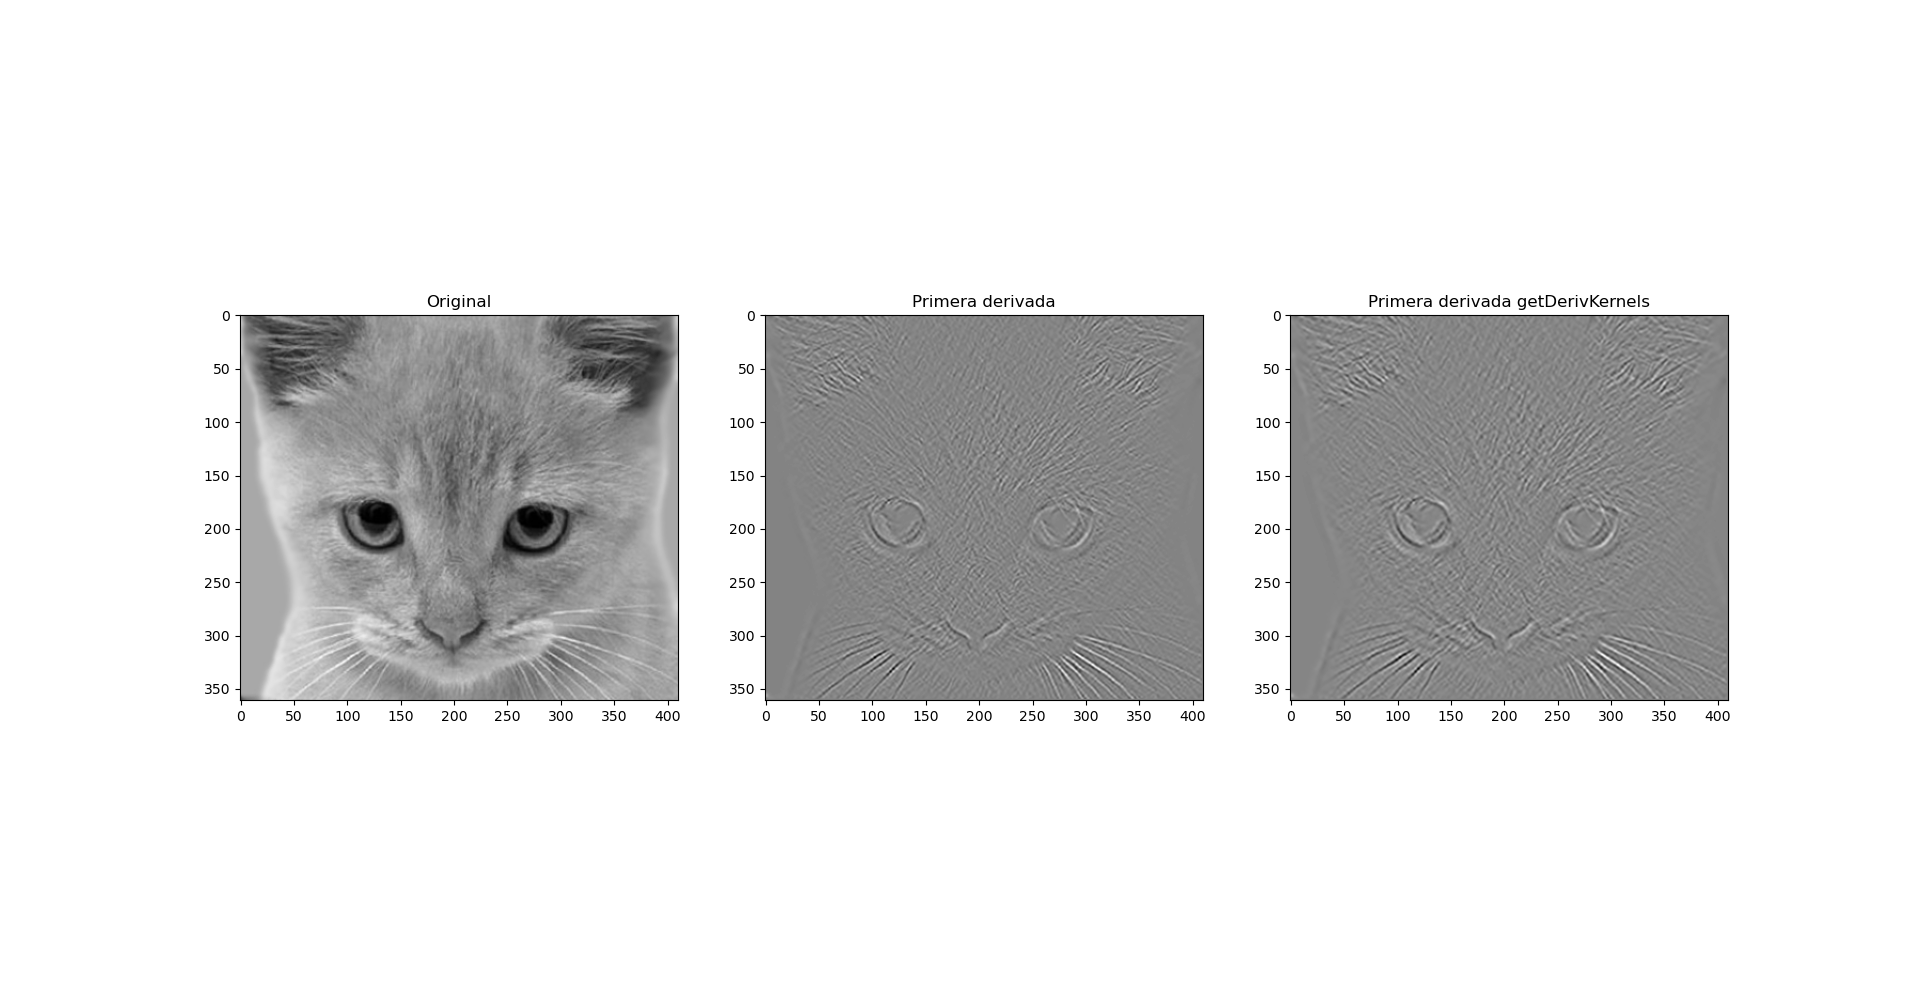
\includegraphics[width=\textwidth]{1d-1s7.png}
 		 \caption{Comparación máscaras primera derivada con tamaño de máscara 7.}
  		\label{fig:ej1d}

\end{figure}

\begin{figure}[H]
  \centering
      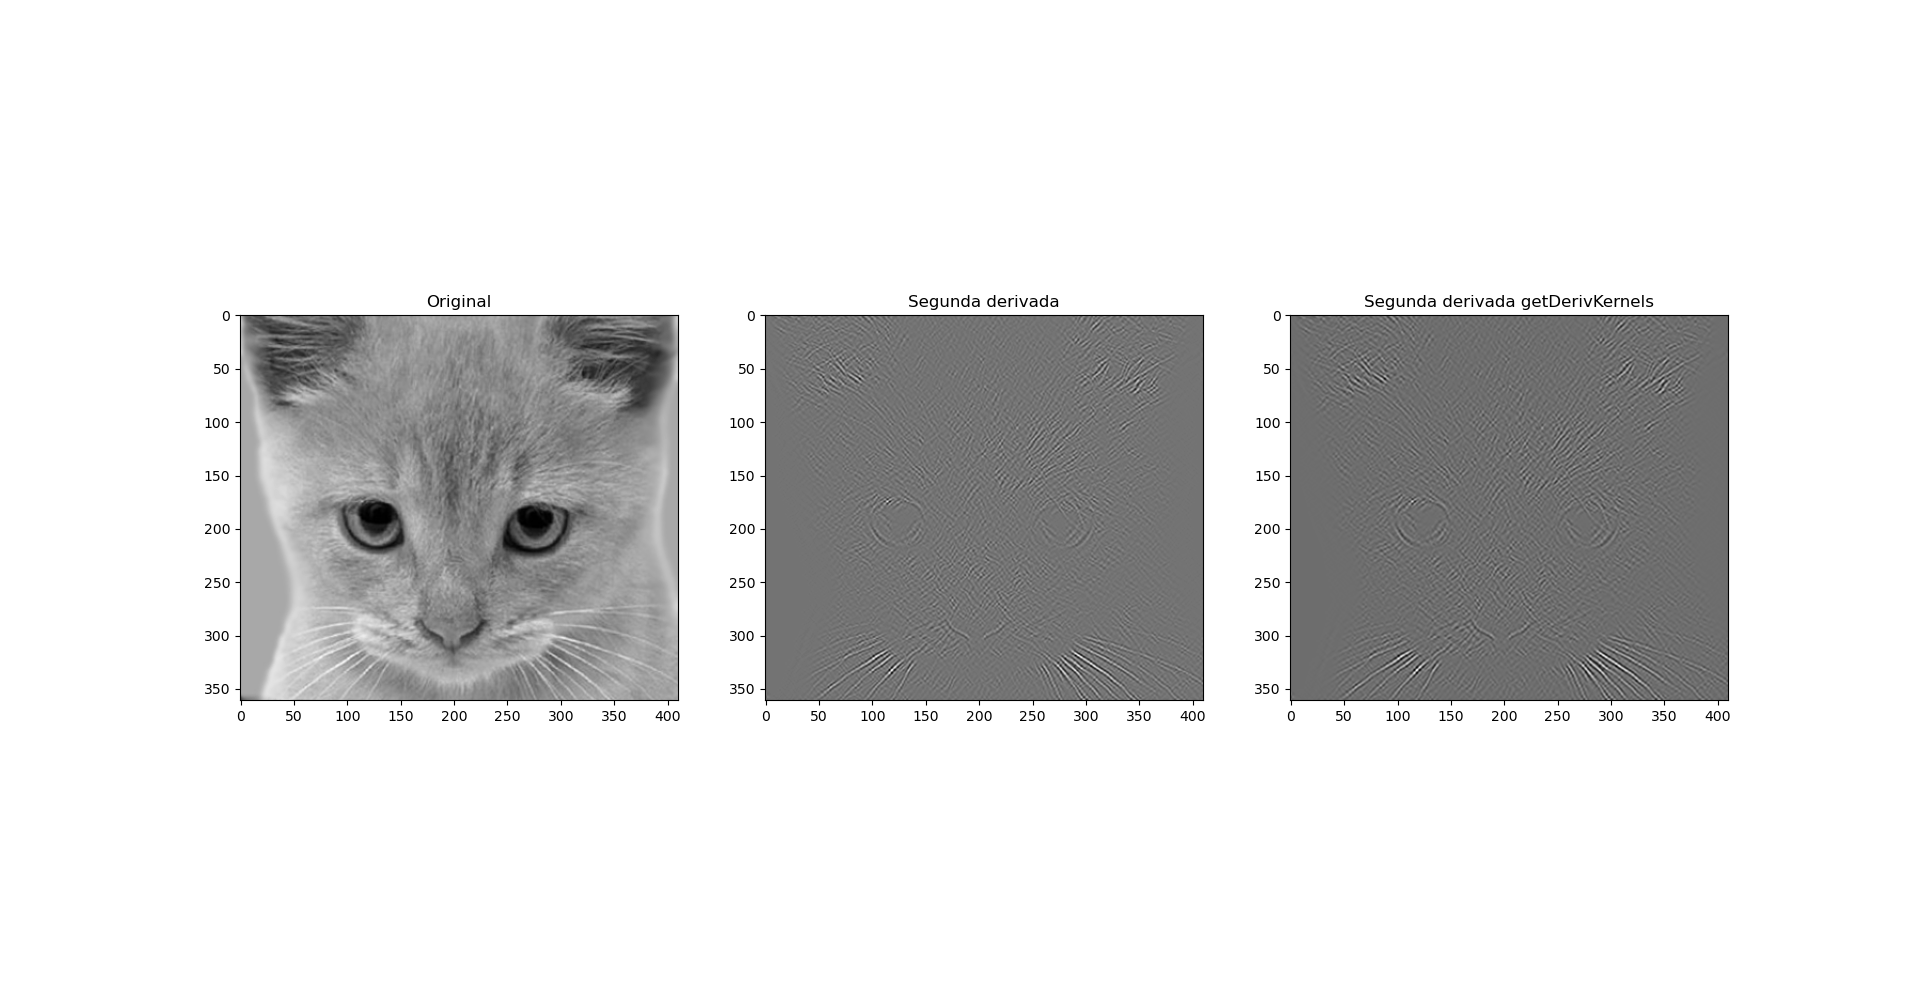
\includegraphics[width=\textwidth]{1d-2s7.png}
 		 \caption{Comparación máscaras segunda derivada con tamaño de máscara 7.}
  		\label{fig:ej1d}

\end{figure}

\subsection{Máscaras Laplacianas}

Como sabemos, la máscara laplaciana es la suma de la segunda derivada de la gaussiana con respecto de $x$ y la segunda derivada de la gaussiana con respecto de $y$, y tras esto normalizamos la suma multiplicandola por $\sigma^2$. Como sabemos de teoría, la segunda derivada de la gaussiana es simétrica de $x$ y de $y$.

Por este motivo, de cara a calcular la imagen con la máscara laplaciana aplicaremos una convolución de la imagen con la máscara de la segunda derivada como máscara horizontal y la máscara gaussiana como máscara vertical, obteniendo la imagen que llamaremos $G_{xx}$, por otro lado obtendremos la imagen $G_{yy}$ aplicando a la imagen original la máscara de la segunda derivada como máscara vertical y la máscara gaussiana como máscara horizontal. Finalmente sumaremos las imagenes $G_{xx}$ y $G_{yy}$ y el resultado lo multiplicaremos por $\sigma^2$, de forma que esta será la imagen final con la máscara aplicada.

Por último en esta función finalmente normalizaremos la imagen en el rango [0-1] para su correcta visualización.


\begin{figure}[H]
  \centering
      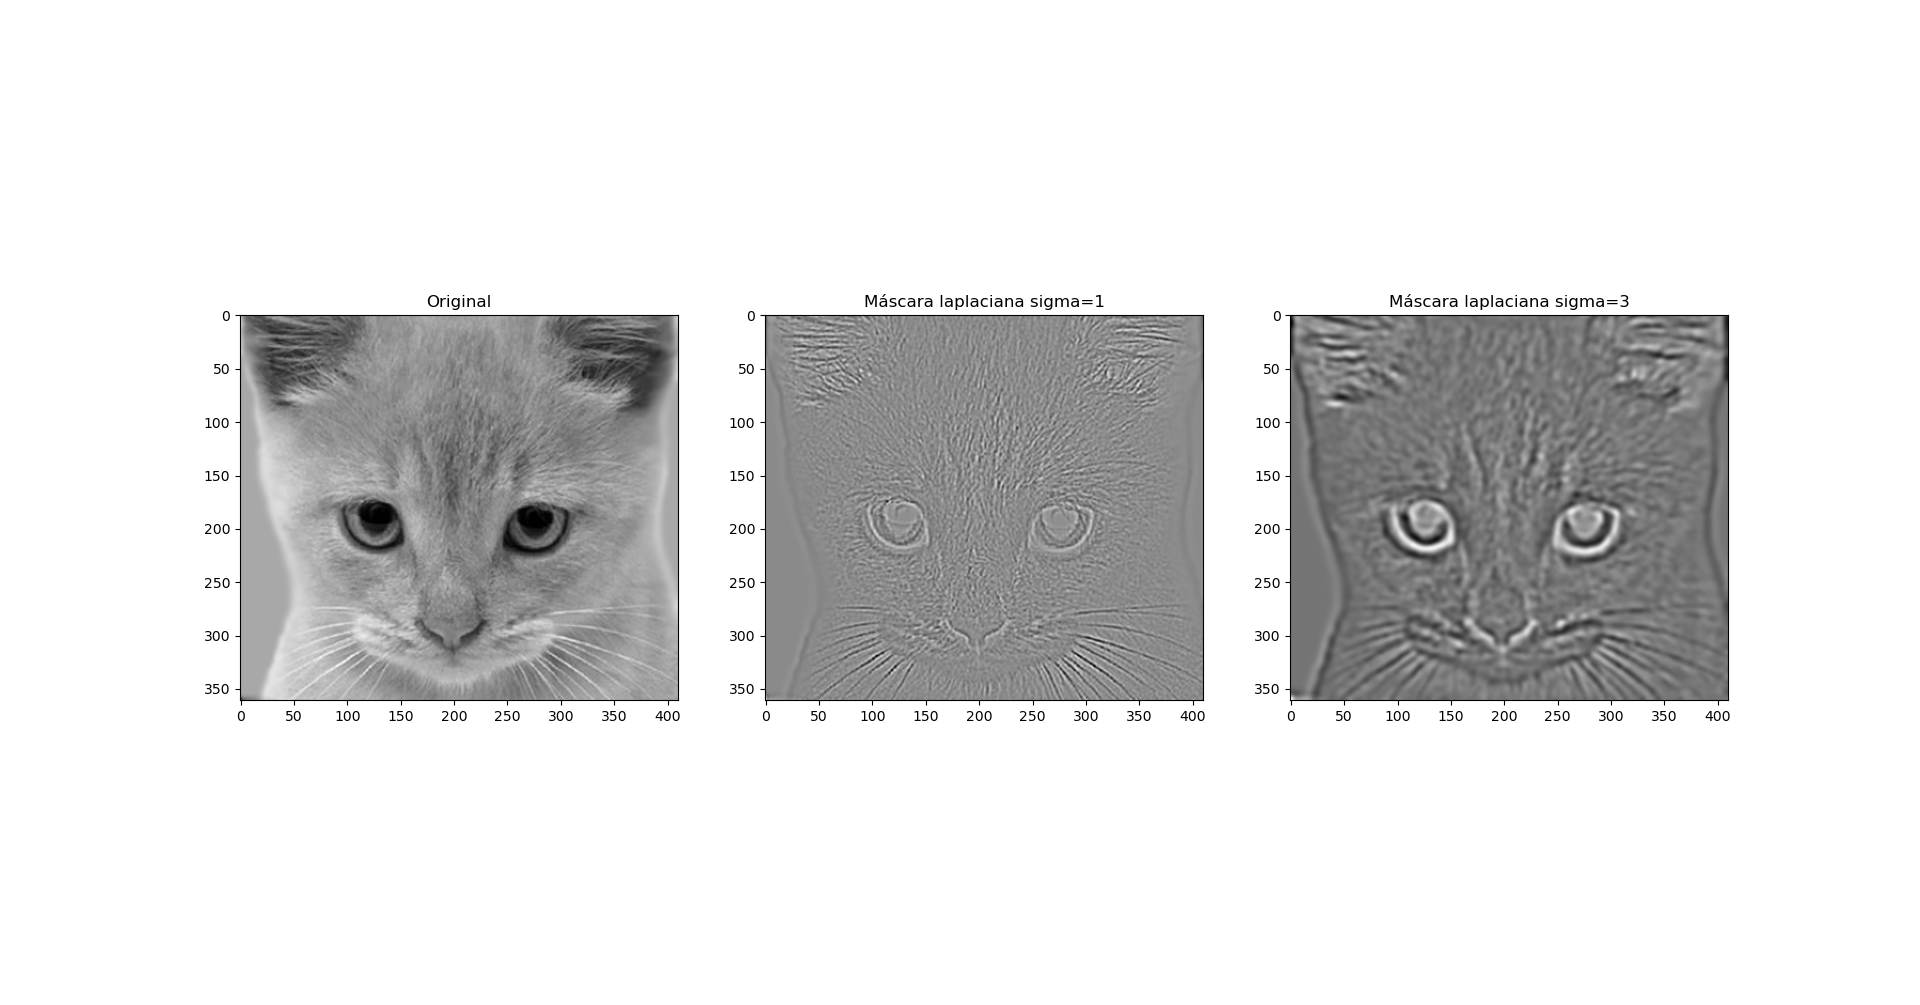
\includegraphics[width=\textwidth]{ej1d.png}
 		 \caption{Máscara laplaciana con sigma 1 y con sigma 3.}
  		\label{fig:ej1d}

\end{figure}



\section{Ejercicio 2: Pirámides}

En este ejercicio se nos pide crear dos tipos de pirámides, la Gaussiana y la Laplaciana, de al menos cuatro niveles (cuatro subsamples, la imagen original cuenta como nivel 0). Para esto se pueden utilizar los métodos de OpenCV pyrUp y pyrDown, sin embargo yo he realizado una implementación propia y las he comparado con la implementación de OpenCV.

\subsection{Pirámide Gaussiana}

La construcción de la pirámide gaussiana se basa reescalar una imagen a la mitad en cada nivel, sin embargo, el hacer directamente ese reescalado hace que se añada ruido a la imagen resultante, y por lo tanto modificando la información de la imagen reescalada. Para evitar esto, antes de reescalar la imagen se aplica un alisamiento utilizando una máscara gaussiana antes de reescalar la imagen.

De cara a obtener la pirámide gaussiana he implementado la función \texttt{piramide\_gaussiana}, que recibe como parámetros una imagen, el número de niveles que tendrá la pirámide, por defecto 4, el sigma a utilizar para el alisamiento antes de reescalar al siguiente nivel, por defecto 1, y el tipo de borde a utilizar al aplicar el alisamiento, por defecto \texttt{cv.BORDER\_REPLICATE}, es decir, réplica de bordes.

Esta función devolverá una lista con las imágenes que conforman la pirámide.

La función se basa en calcular la máscara gaussiana con el sigma dado, y tras esto, para cada nivel de la pirámide, aplicar dicha máscara al nivel anterior y formar un nuevo nivel con la imagen alisada por la máscara gaussiana, pero utilizando solo las filas y columnas pares, de forma que el tamaño de la imagen es de la mitad tanto en filas como en columnas.


Debido a que MatPlotLib escala las imágenes para que se muestren todas del mismo tamaño, he creado la función \texttt{apilar\_piramide} que dada una piramide, apila de forma vertical los niveles (a partir del uno) de la pirámide, y apila el nivel cero (imagen horizontal) por la derecha, de forma que el resultado sea una única imagen a mostrar y se visualice con las proporciones correctas.

El resultado obtenido es el siguiente:


\begin{figure}[H]
  \centering
      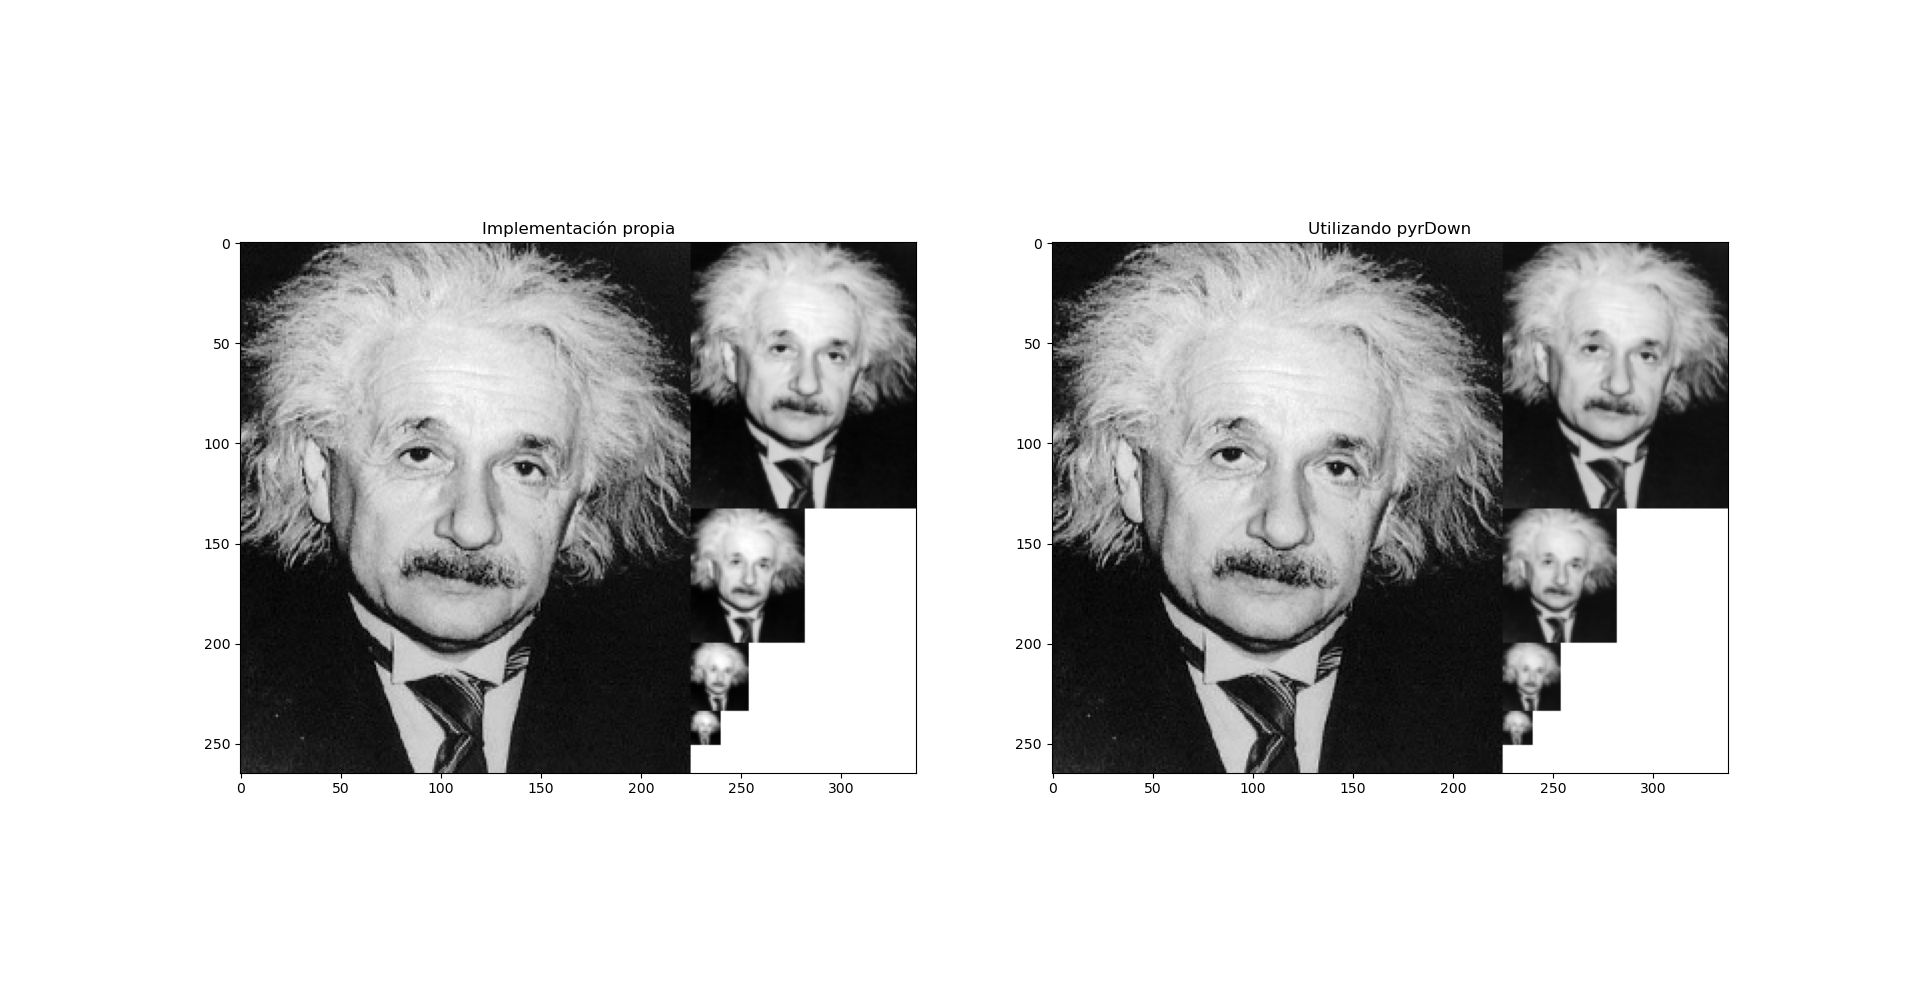
\includegraphics[width=\textwidth]{ej2AG.png}
 		 \caption{Pirámide gaussiana usando la implementación propia y utilizando OpenCV.}
  		\label{fig:ej2ag}

\end{figure}

Observamos como el resultado es equivalente al utilizado con pyrDown, por lo que podemos suponer que es correcto.

\subsection{Pirámide Laplaciana}

La construcción de la pirámide laplaciana se basa en, teniendo la pirámide gaussiana de la imagen, calcular un nivel $x$ de la pirámide laplaciana restando el nivel $x$ de la pirámide gaussiana con el nivel $x+1$ de la pirámide gaussiana reescalado, de forma que tenga las mismas dimensiones que el nivel $x$ para poder restar dichas imagenes. Por este motivo, el nivel más alto (imagen más pequeña de la pirámide), siempre será el nivel más alto de la pirámide gaussiana.

Para obtener esta pirámide he desarrollado la función \texttt{piramide\_laplaciana}, que recibe por parámetro una imagen, el número de niveles, por defecto cuatro, el valor de sigma, por defecto uno, y la forma de añadir el borde, por defecto réplica.

Esta función describe el procedimiento explicado en el primer párrafo, utilizando el método \texttt{resize} de OpenCV para reescalar los niveles de la pirámide gaussiana, y devuelve una lista con la pirámide.

De nuevo, para poder visualizar la pirámide con las proporciones reales he utilizado la función \texttt{apilar\_piramide} comentada en el apartado anterior. El resultado es el siguiente:

\begin{figure}[H]
  \centering
      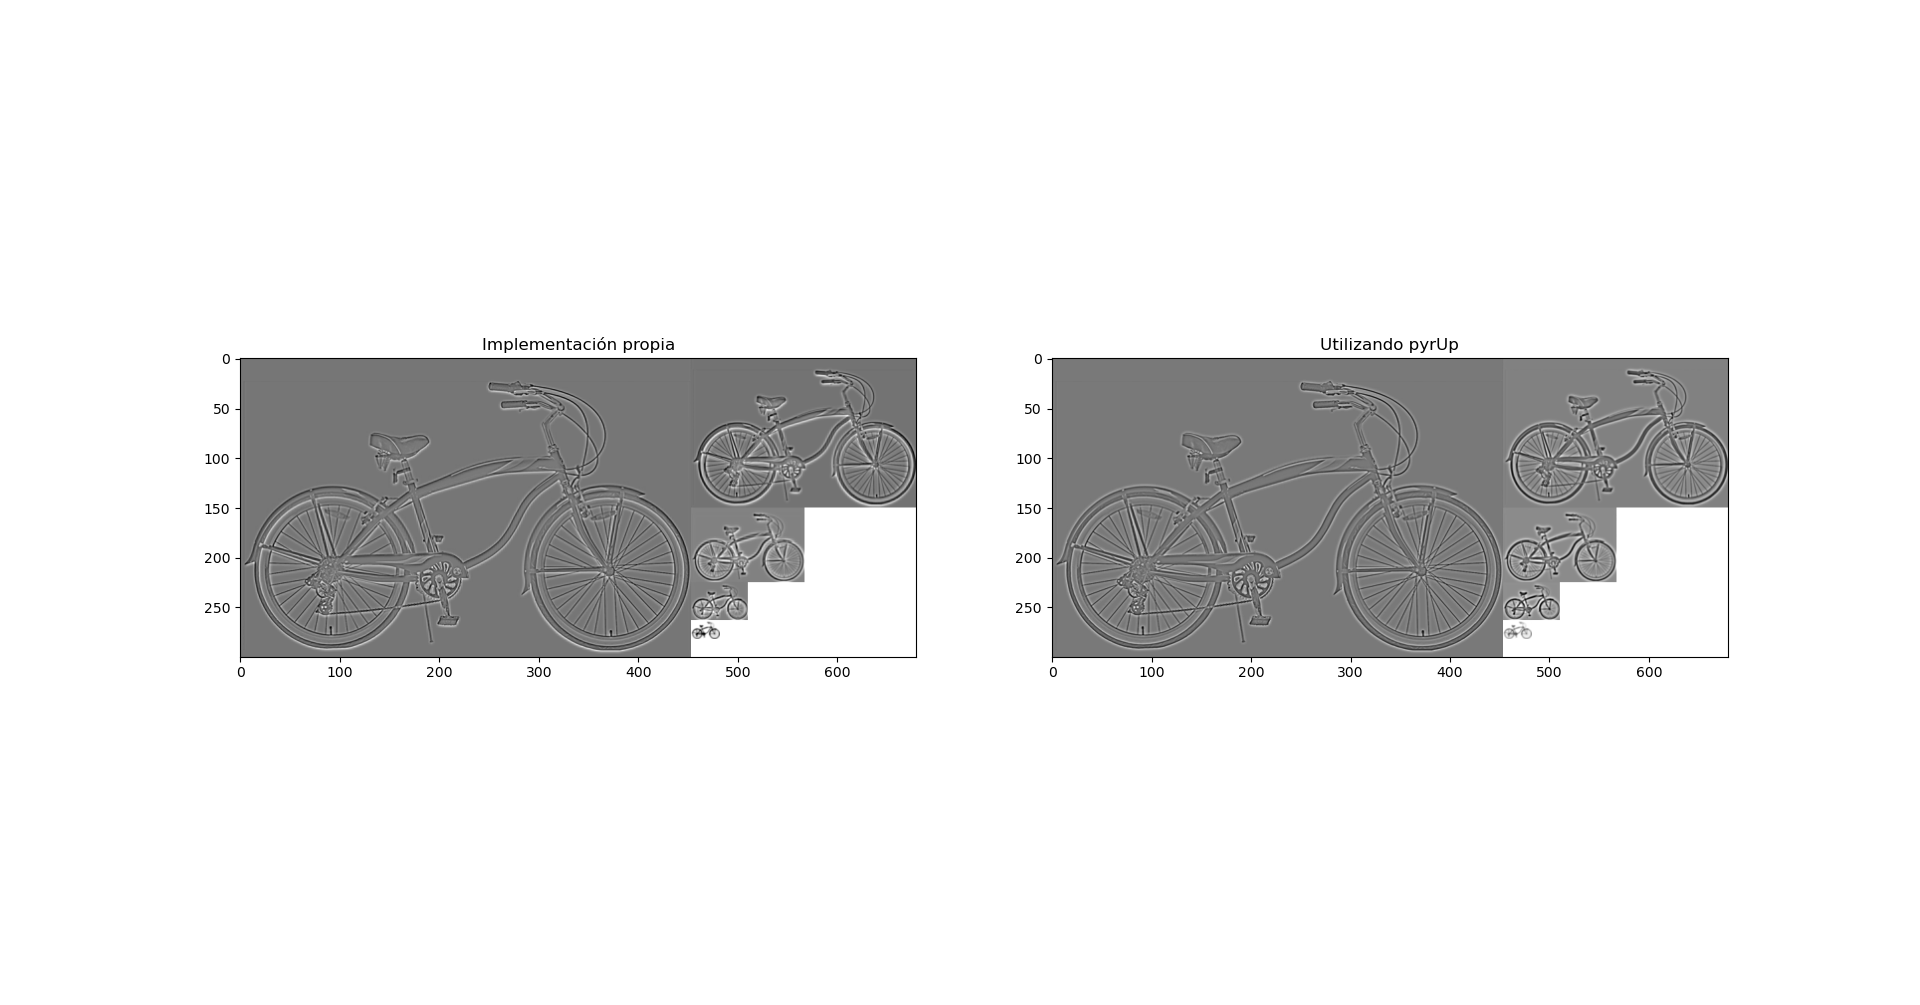
\includegraphics[width=\textwidth]{ej2AL.png}
 		 \caption{Pirámide laplaciana usando la implementación propia y utilizando OpenCV.}
  		\label{fig:ej2al}

\end{figure}

En este caso vemos como el resultado también es equivalente a utilizar pyrUp, sin embargo en este ejemplo vemos como nuestra propia implementación da unos mejores resultados al marcar mejor los bordes, debido a que nosotros utilizamos las funciones exactas y no una aproximación, como hace OpenCV, y precisamente en esta operación donde se muestran las diferencias entre como se aplica el alisado y el reescalado vemos que se hace más clara la diferencia entre utilizar el método exacto y una aproximación.

\section{Ejercicio 3: Imágenes híbridas}

Este ejercicio se basa en el trabajo sobre imágenes híbridas\cite{img_hibridas}, en el cual se explica que en una imagen, si la observamos desde cerca el ojo humano se centra en las frecuencas altas de la imagen, mientras que si la observamos desde cierta distancia se centra en las frecuencias bajas, por lo tanto podemos aprovechar esto para crear imágenes en las que desde cerca se observen ciertos objetos y desde lejos otros distintos.


Para realizar este ejercicio he usado las máscaras gaussianas, que son máscaras de paso bajo, es decir, mantienen las frecuencias bajas de la imagen, y eliminan las frecuencias altas. De esta forma, dadas dos imágenes A y B, de la imagen A obtenemos la imagen con frecuencias bajas Abajas aplicando una máscara gaussiana, y obtenemos la imagen B con frecuencias altas Baltas obteniendo una imagen temporal Btmp con frecuencias bajas al aplicarle una máscara gaussiana, y esa imagen restandola a la imagen original B, de forma que eliminamos las frecuencias bajas y mantenemos las altas. Tras obtener las imagenes con altas y bajas frecuencias, simplemente las sumamos.


Por lo tanto, he desarrollado una función \texttt{crear\_imagen\_hibrida} que recibe como parámetros:

\begin{enumerate}
	\item Imágen en la que queremos mantener las frecuencias bajas.
	\item Imágen en la que queremos mantener las frecuencias altas.
	\item Sigma a aplicar a la imagen para obtener frecuencias bajas.
	\item Sigma a aplicar a la imagen para obtener frecuencias altas.
	\item Tipo de bordes para aplicar las convoluciones, por defecto réplica.
\end{enumerate}

Esta función simplemente se comporta como he descrito anteriormente, y devuelve tres imágenes, la imagen hibrida, la imagen de bajas frecuencias, y la imagen de altas frecuencias en una lista. Antes de devolver las imágenes las normaliza en el rango [0-1] de cara a su correcta visualización.

De cara a obtener las imágenes híbridas de las imágenes dadas se han escogido los parámtros y que imagen de cada pareja mantendría unas u otras frecuencias de forma empírica.

Estos son los resultados y la comparación de las imágenes híbridas con las imágenes con frecuencias bajas y altas:


\begin{figure}[H]
  \centering
      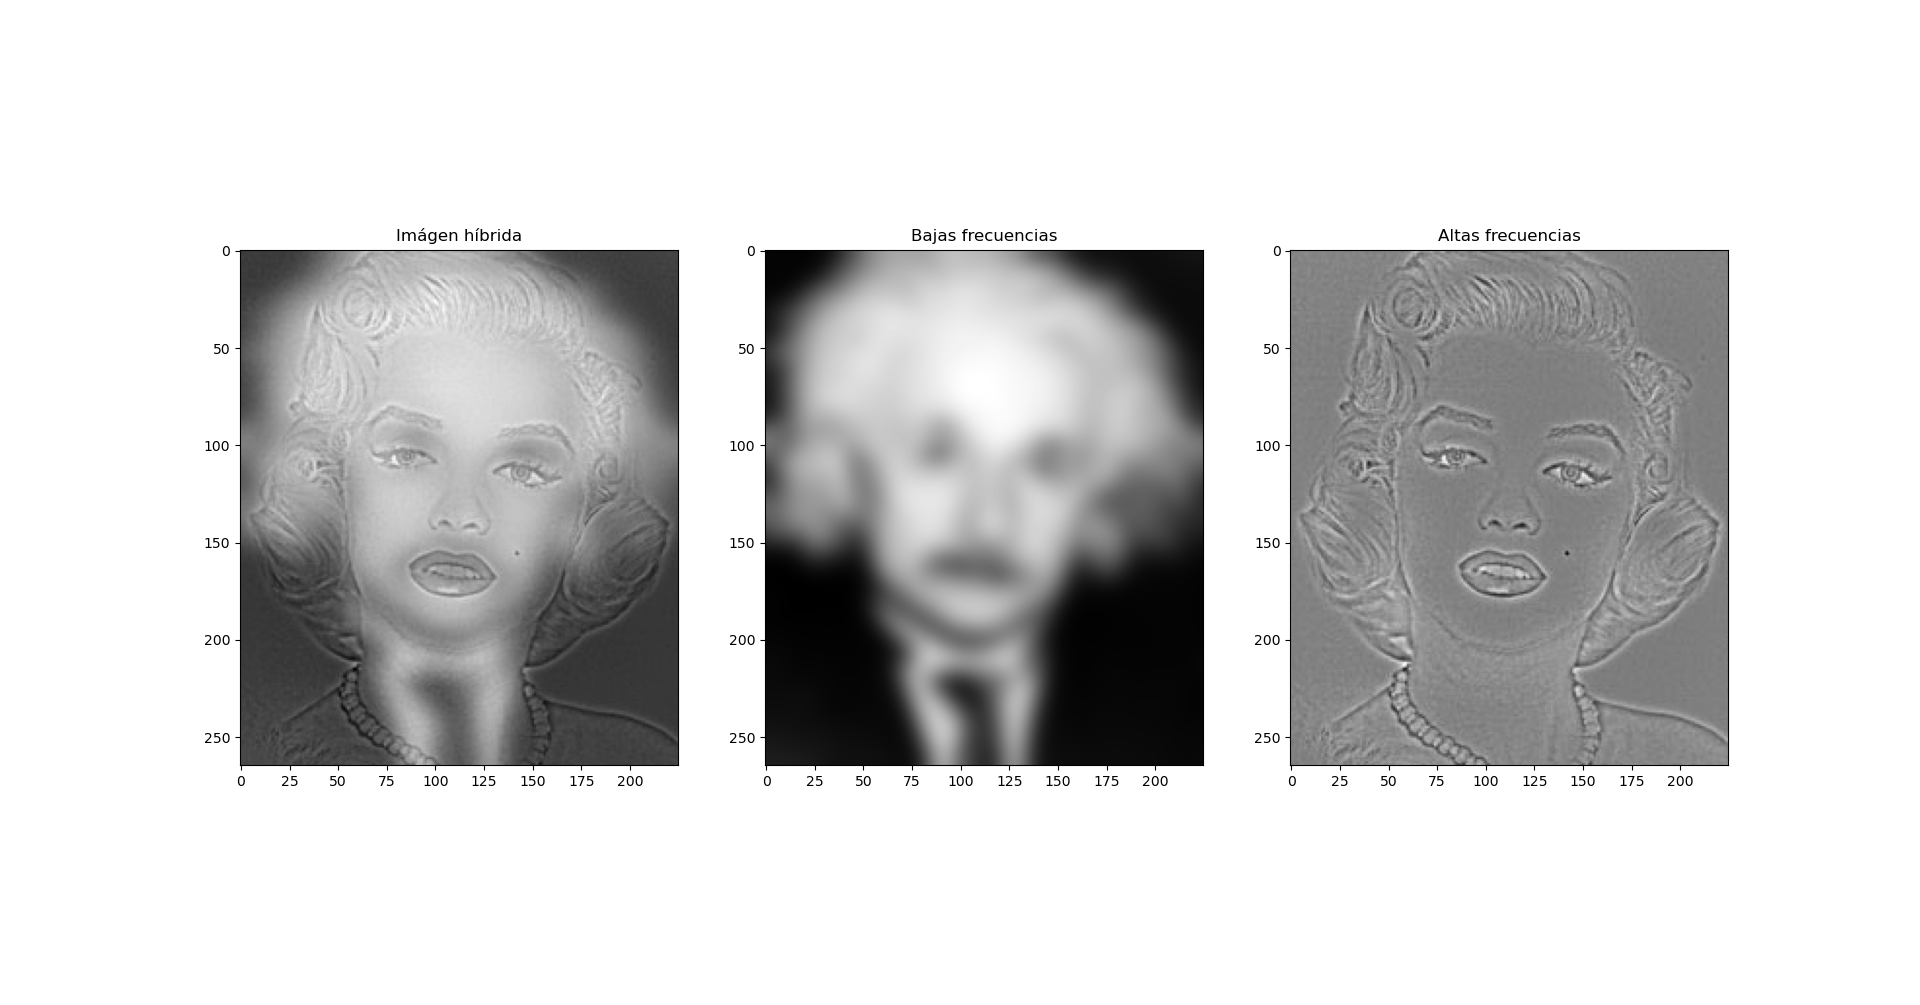
\includegraphics[width=\textwidth]{hibridas/E-M.png}
 		 \caption{Imágen hibrida de Eintein con Marylin.}
  		\label{fig:ej2al}

\end{figure}


\begin{figure}[H]
  \centering
      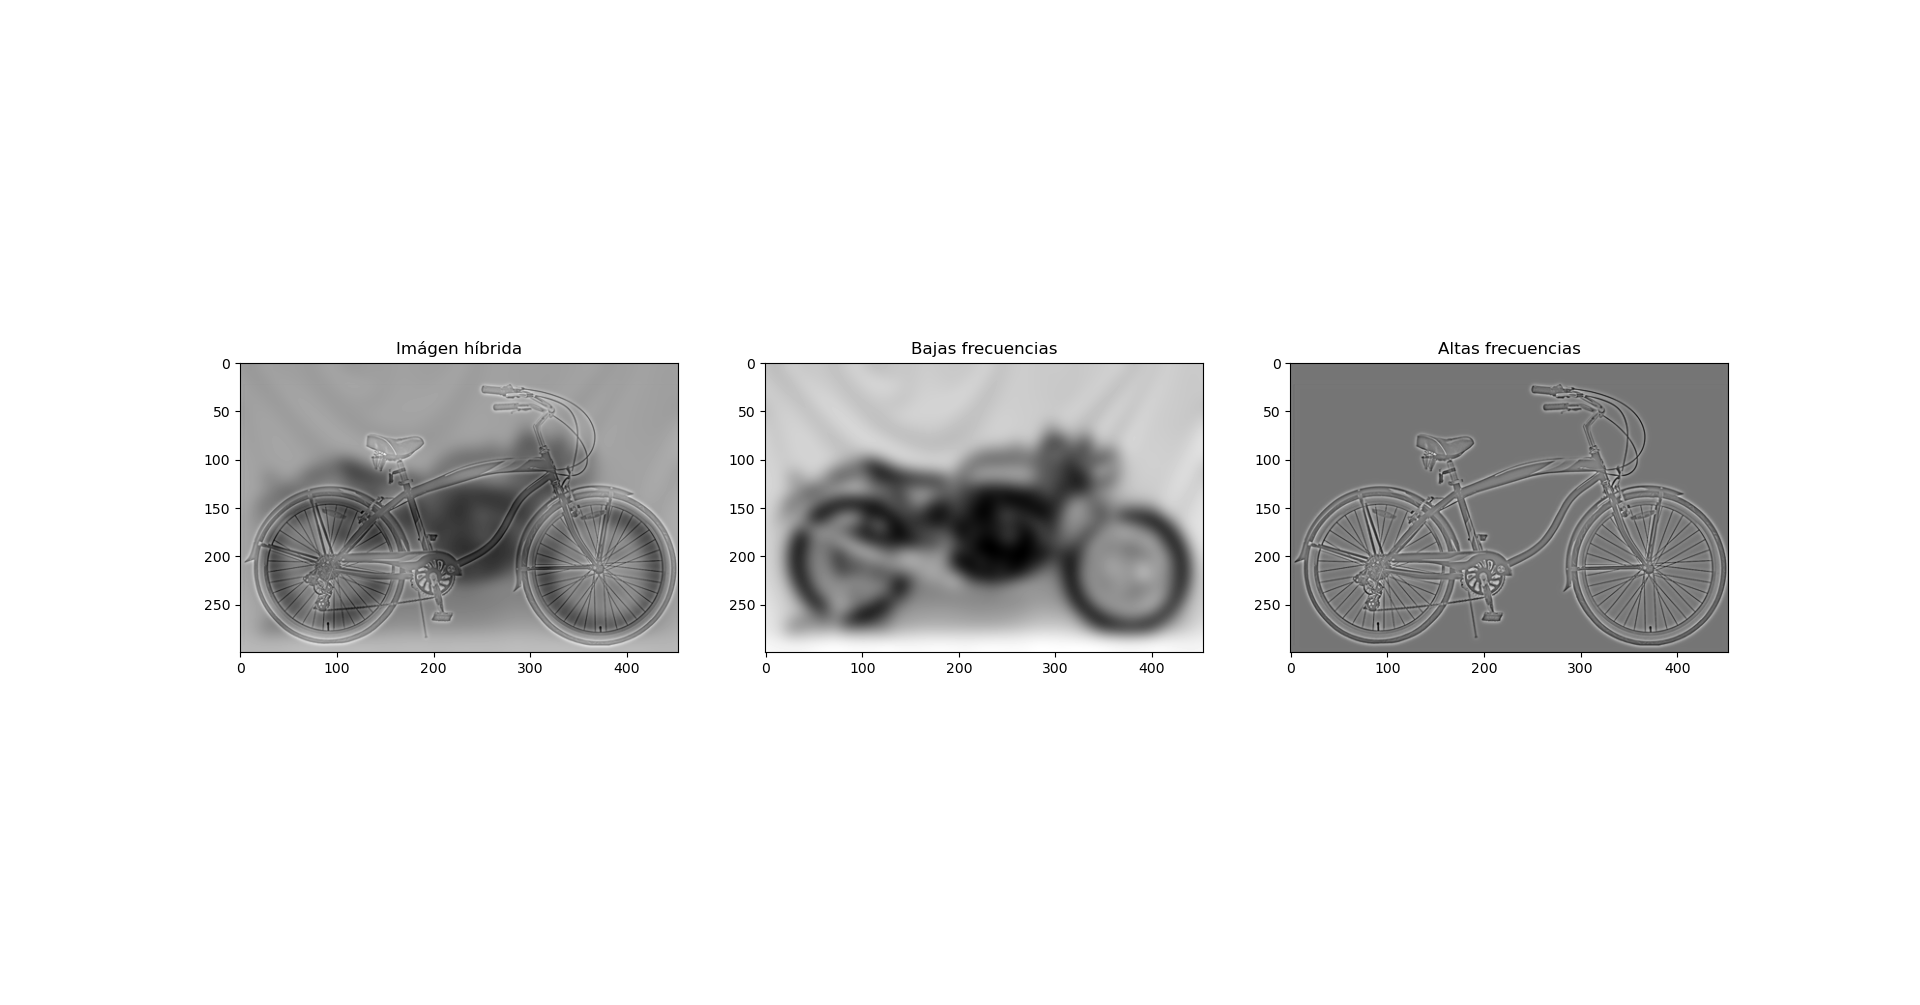
\includegraphics[width=\textwidth]{hibridas/B-M.png}
 		 \caption{Imágen hibrida de una bicicleta con una motocicleta.}
  		\label{fig:ej2al}

\end{figure}


\begin{figure}[H]
  \centering
      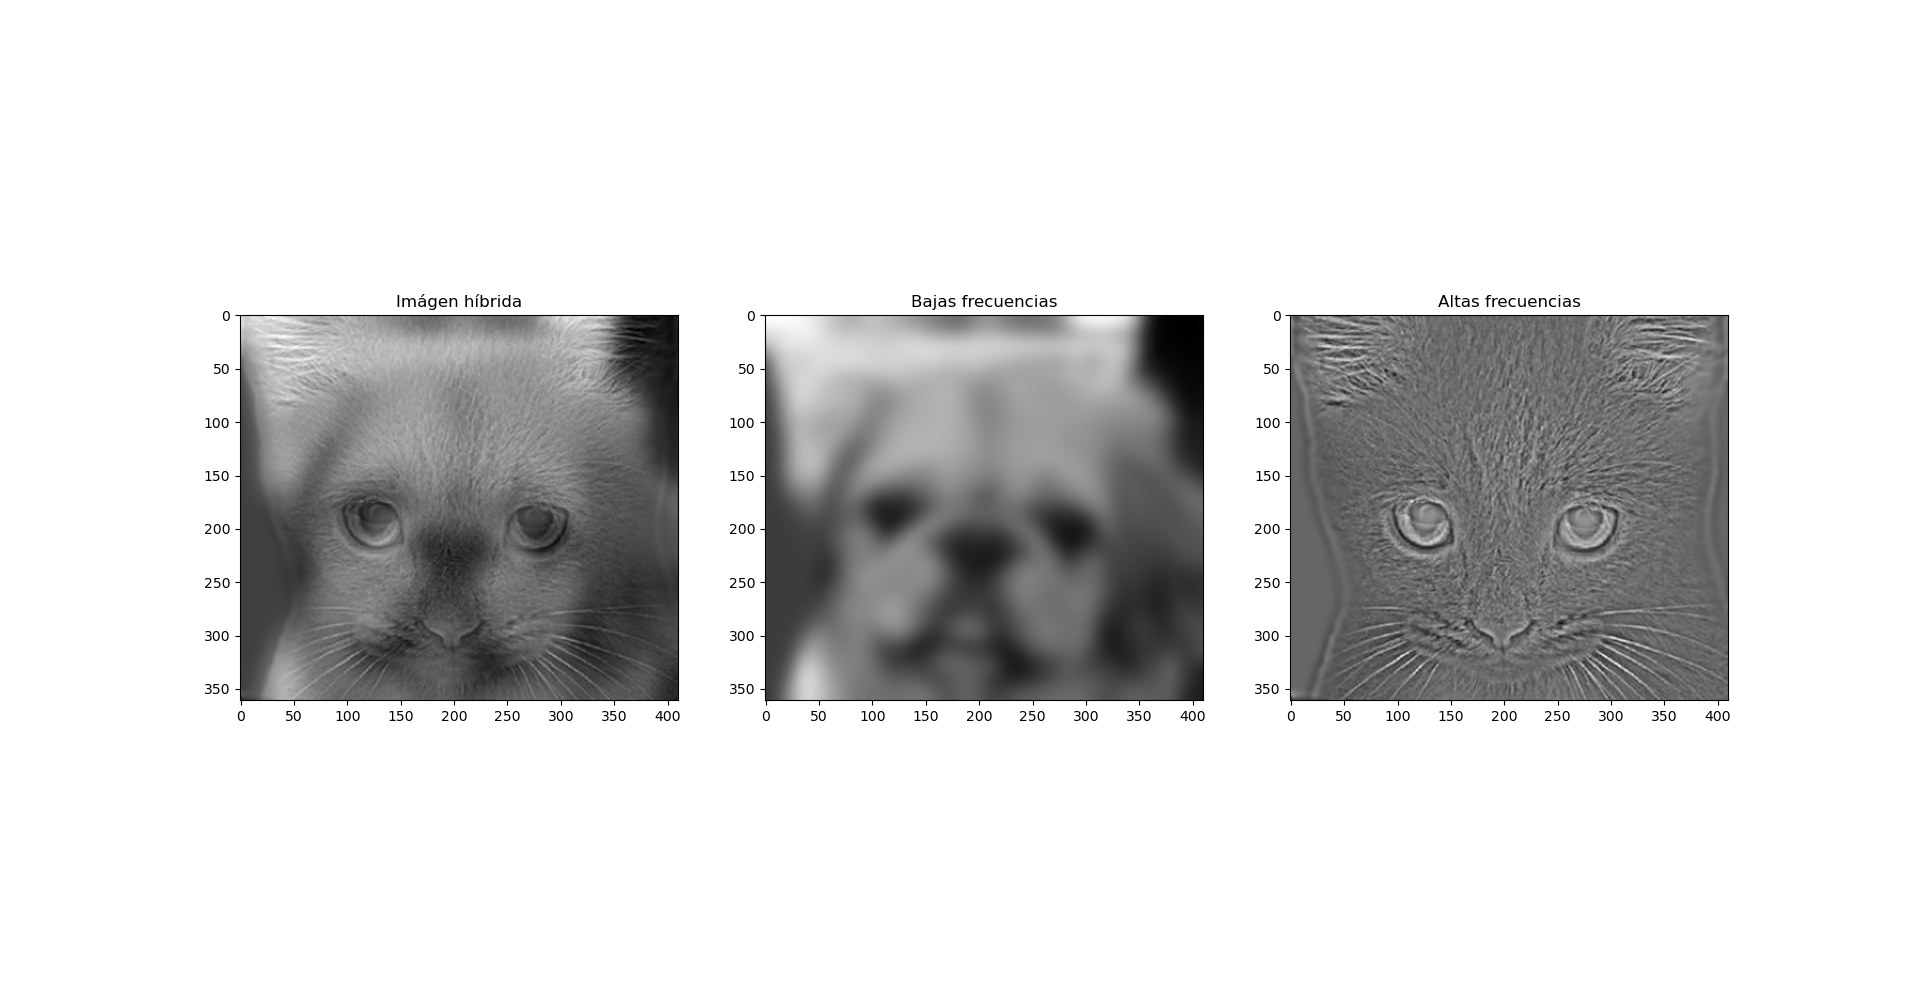
\includegraphics[width=\textwidth]{hibridas/G-P.png}
 		 \caption{Imágen hibrida de un gato y un perro.}
  		\label{fig:ej2al}

\end{figure}


\begin{figure}[H]
  \centering
      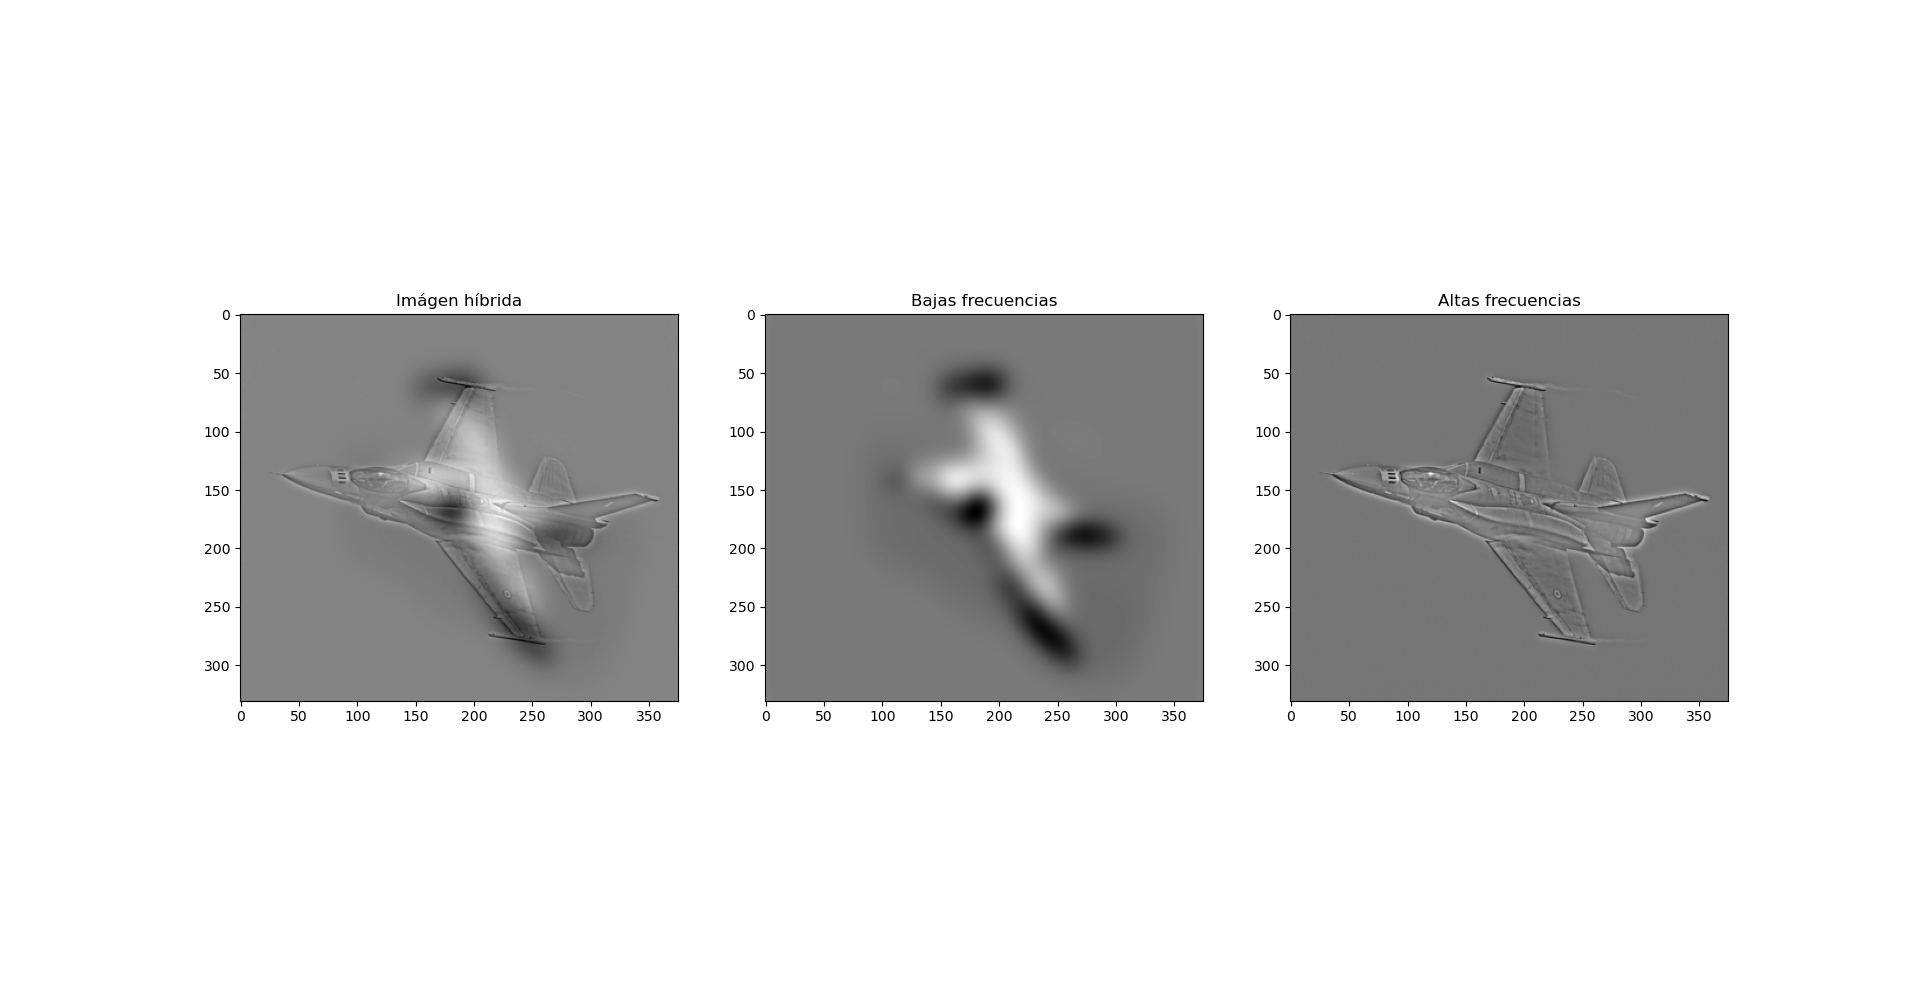
\includegraphics[width=\textwidth]{hibridas/A-P.png}
 		 \caption{Imágen hibrida de un avión y un pájaro.}
  		\label{fig:ej2al}

\end{figure}

\begin{figure}[H]
  \centering
      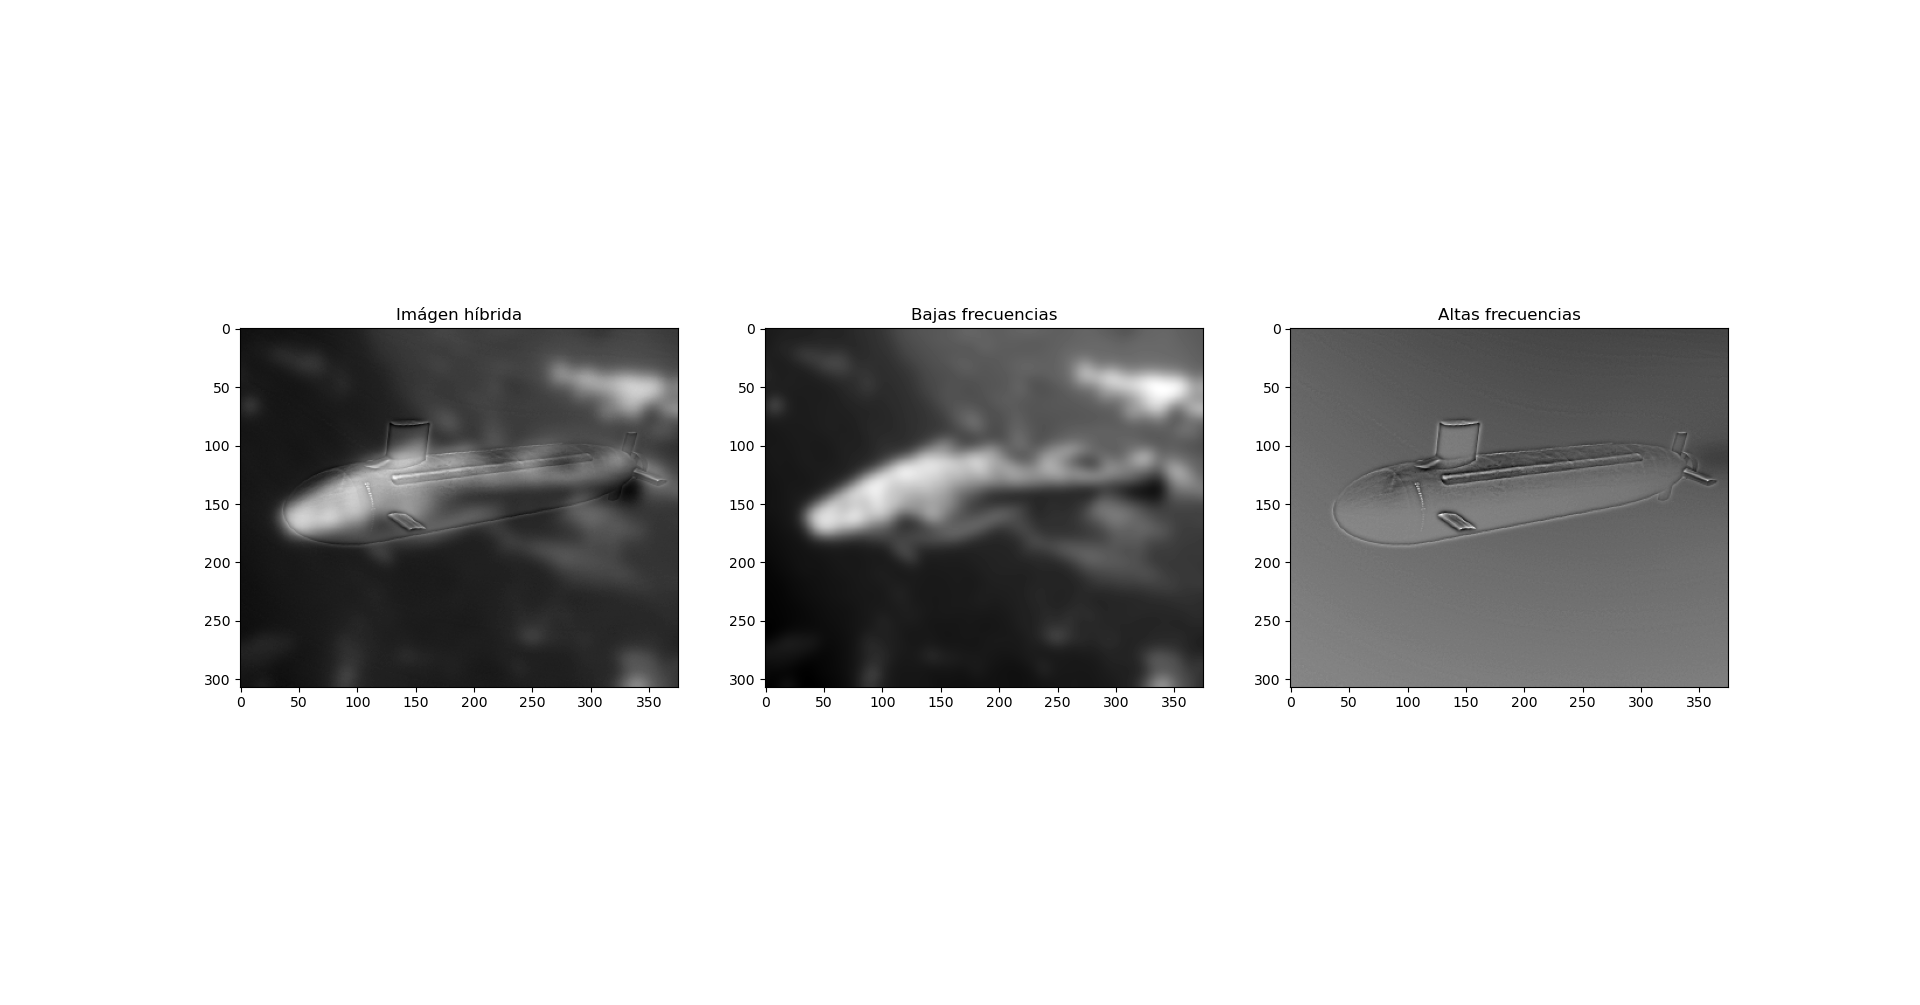
\includegraphics[width=\textwidth]{hibridas/P-S.png}
 		 \caption{Imágen hibrida de un pez y un submarino.}
  		\label{fig:ej2al}

\end{figure}


De cara a que la distinción sea más clara, como nos pide el ejercicio, mostraré la pirámide gaussiana obtenida de las imágenes hibridas utilizando la función desarrollada en el ejercicio 2:



\begin{figure}[H]
  \centering
      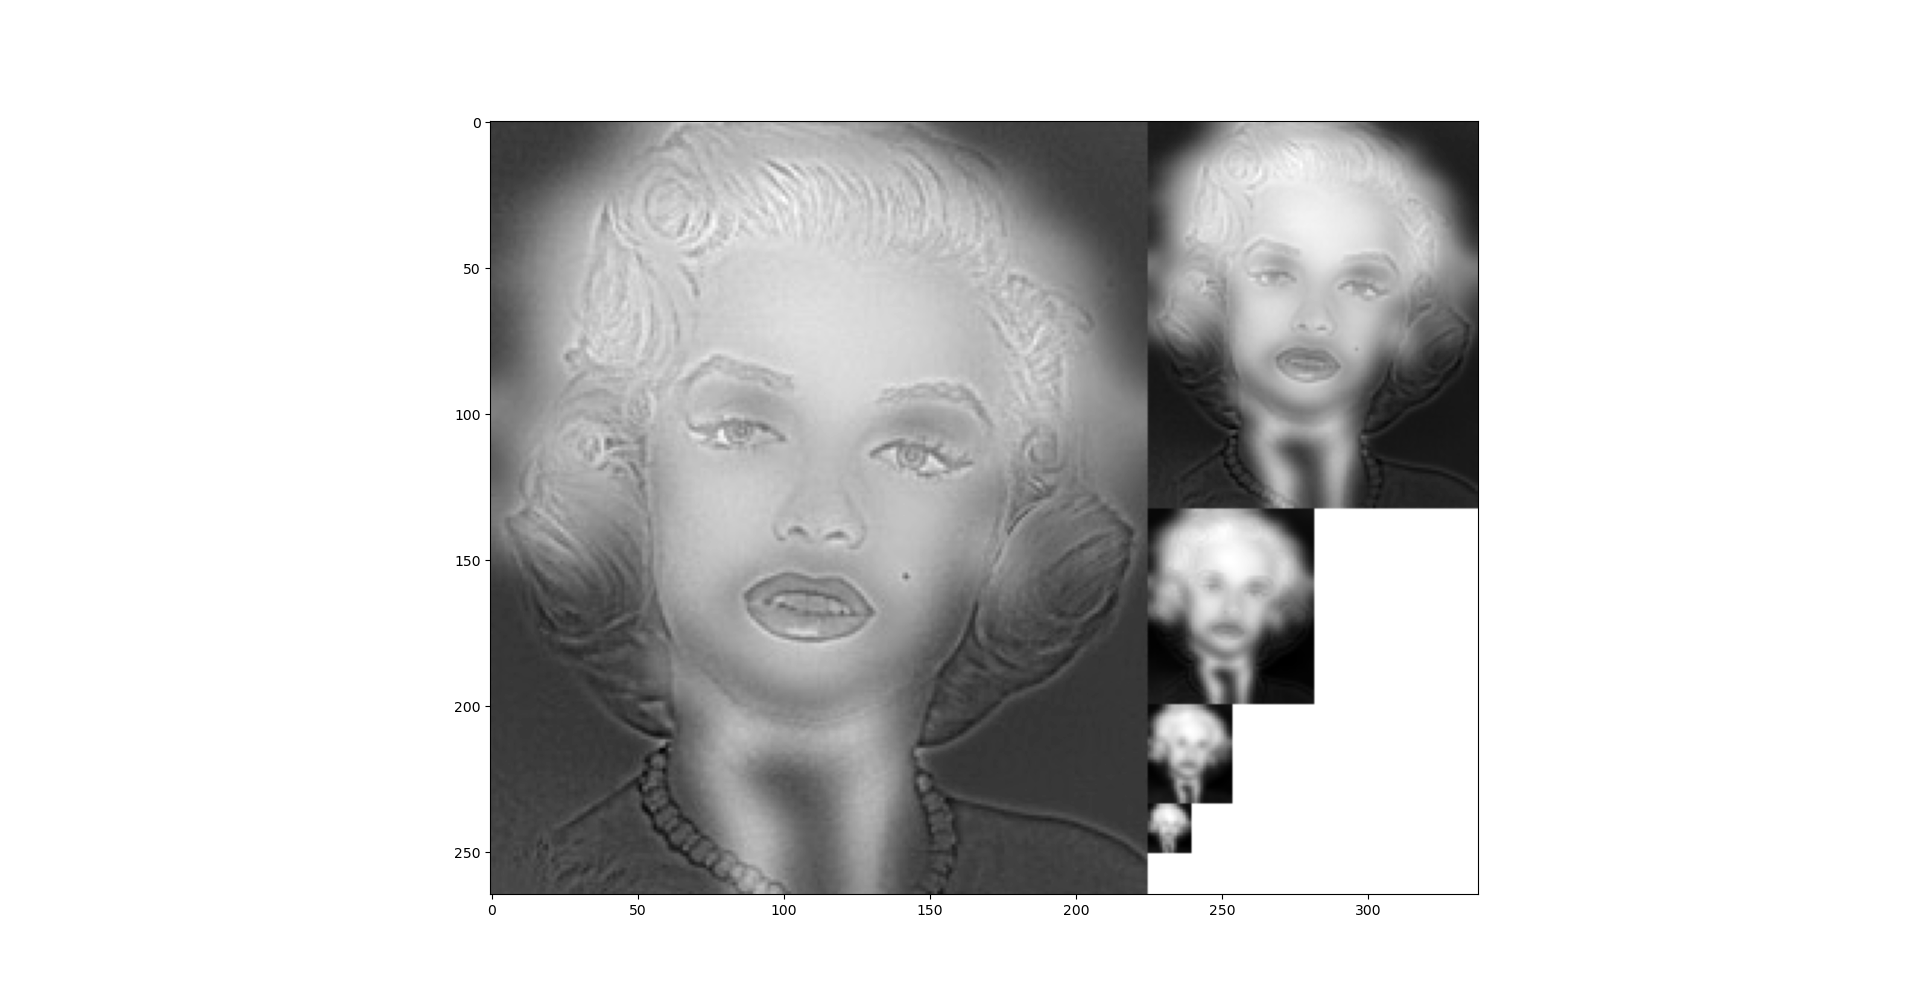
\includegraphics[width=\textwidth]{hibridas/PE-M.png}
 		 \caption{Pirámide de la imágen hibrida de Eintein con Marylin.}
  		\label{fig:ej2al}

\end{figure}


\begin{figure}[H]
  \centering
      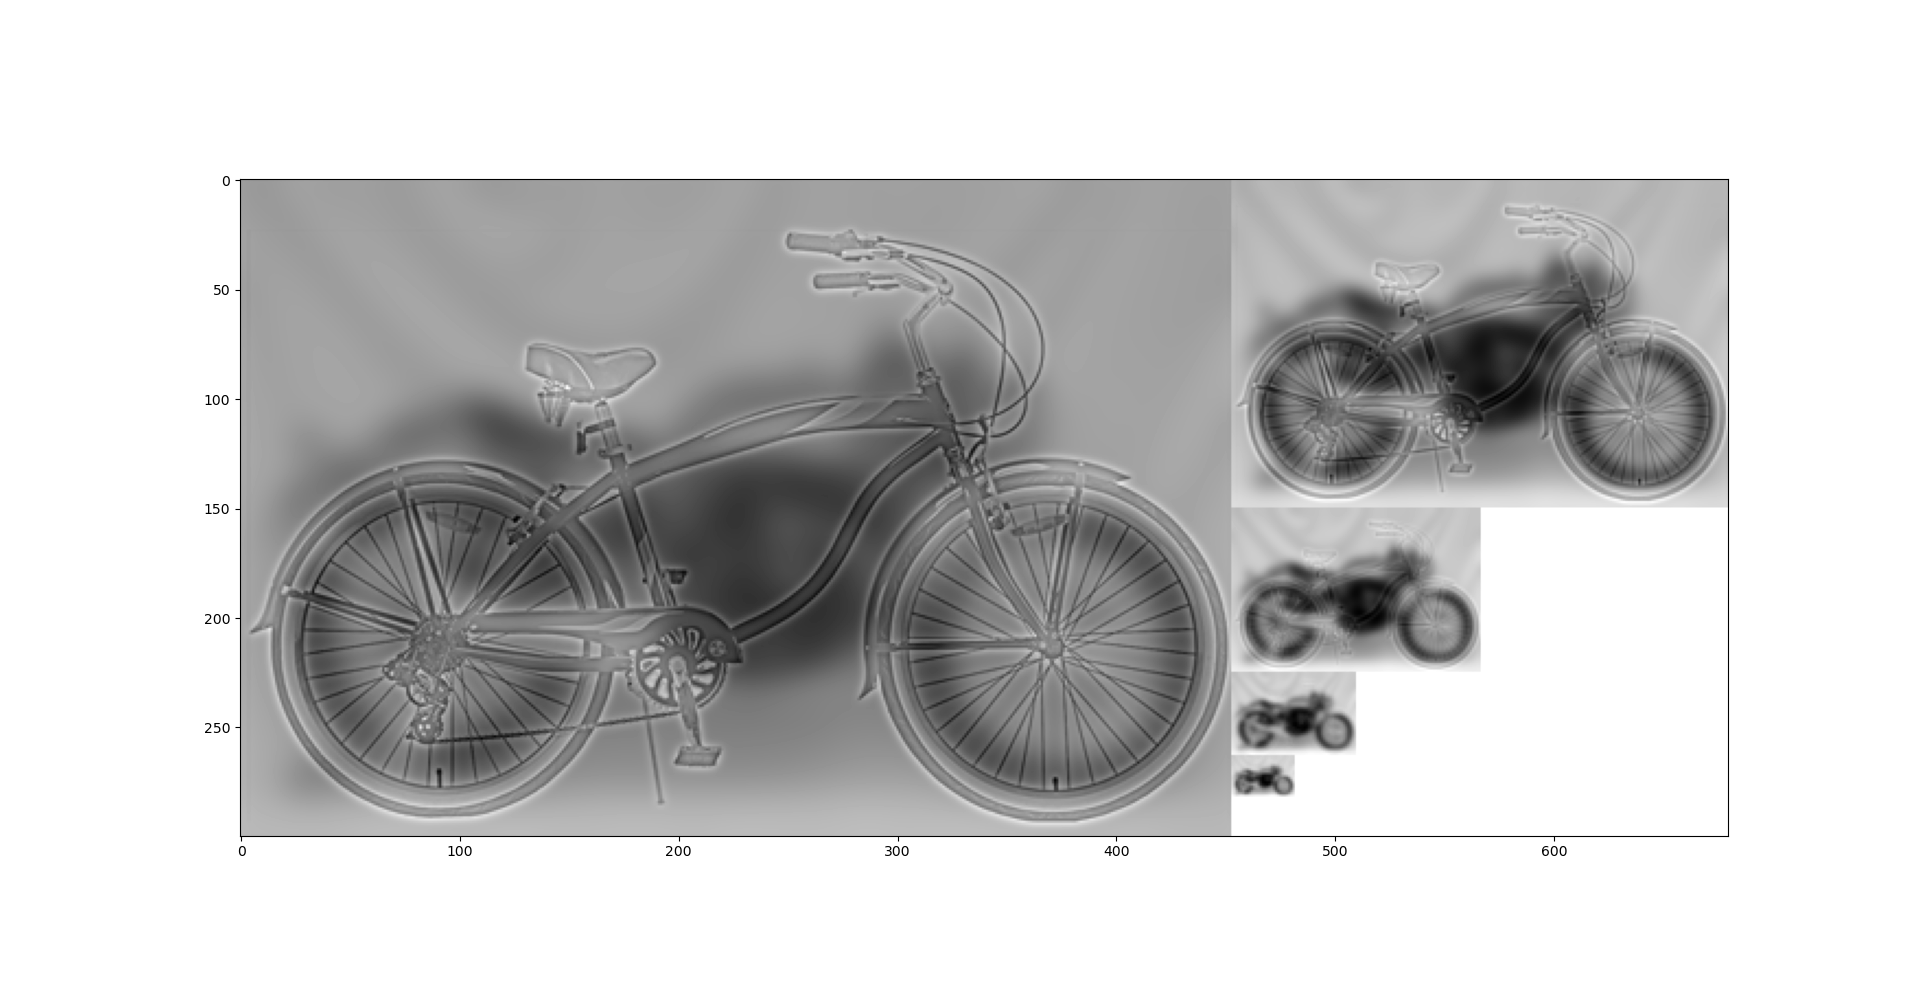
\includegraphics[width=\textwidth]{hibridas/PB-M.png}
 		 \caption{Pirámide de la imágen hibrida de una bicicleta con una motocicleta.}
  		\label{fig:ej2al}

\end{figure}


\begin{figure}[H]
  \centering
      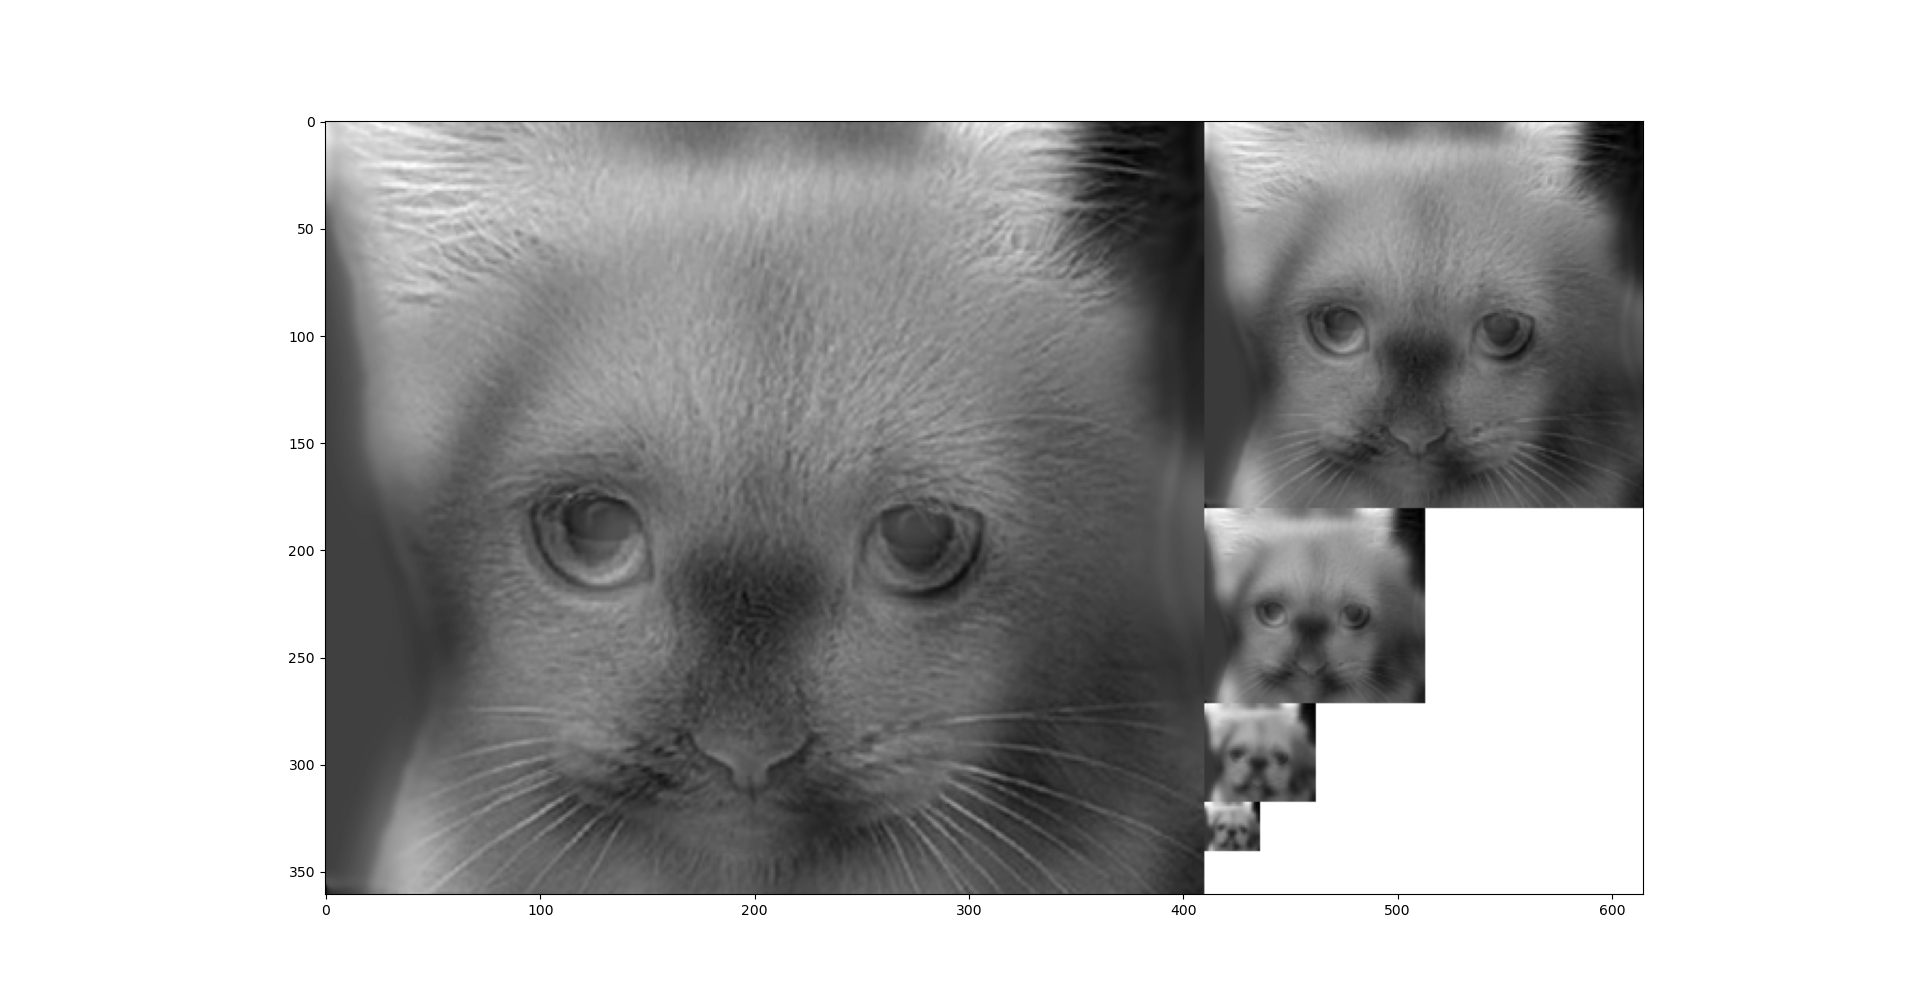
\includegraphics[width=\textwidth]{hibridas/PG-P.png}
 		 \caption{Pirámide de la imágen hibrida de un gato y un perro.}
  		\label{fig:ej2al}

\end{figure}


\begin{figure}[H]
  \centering
      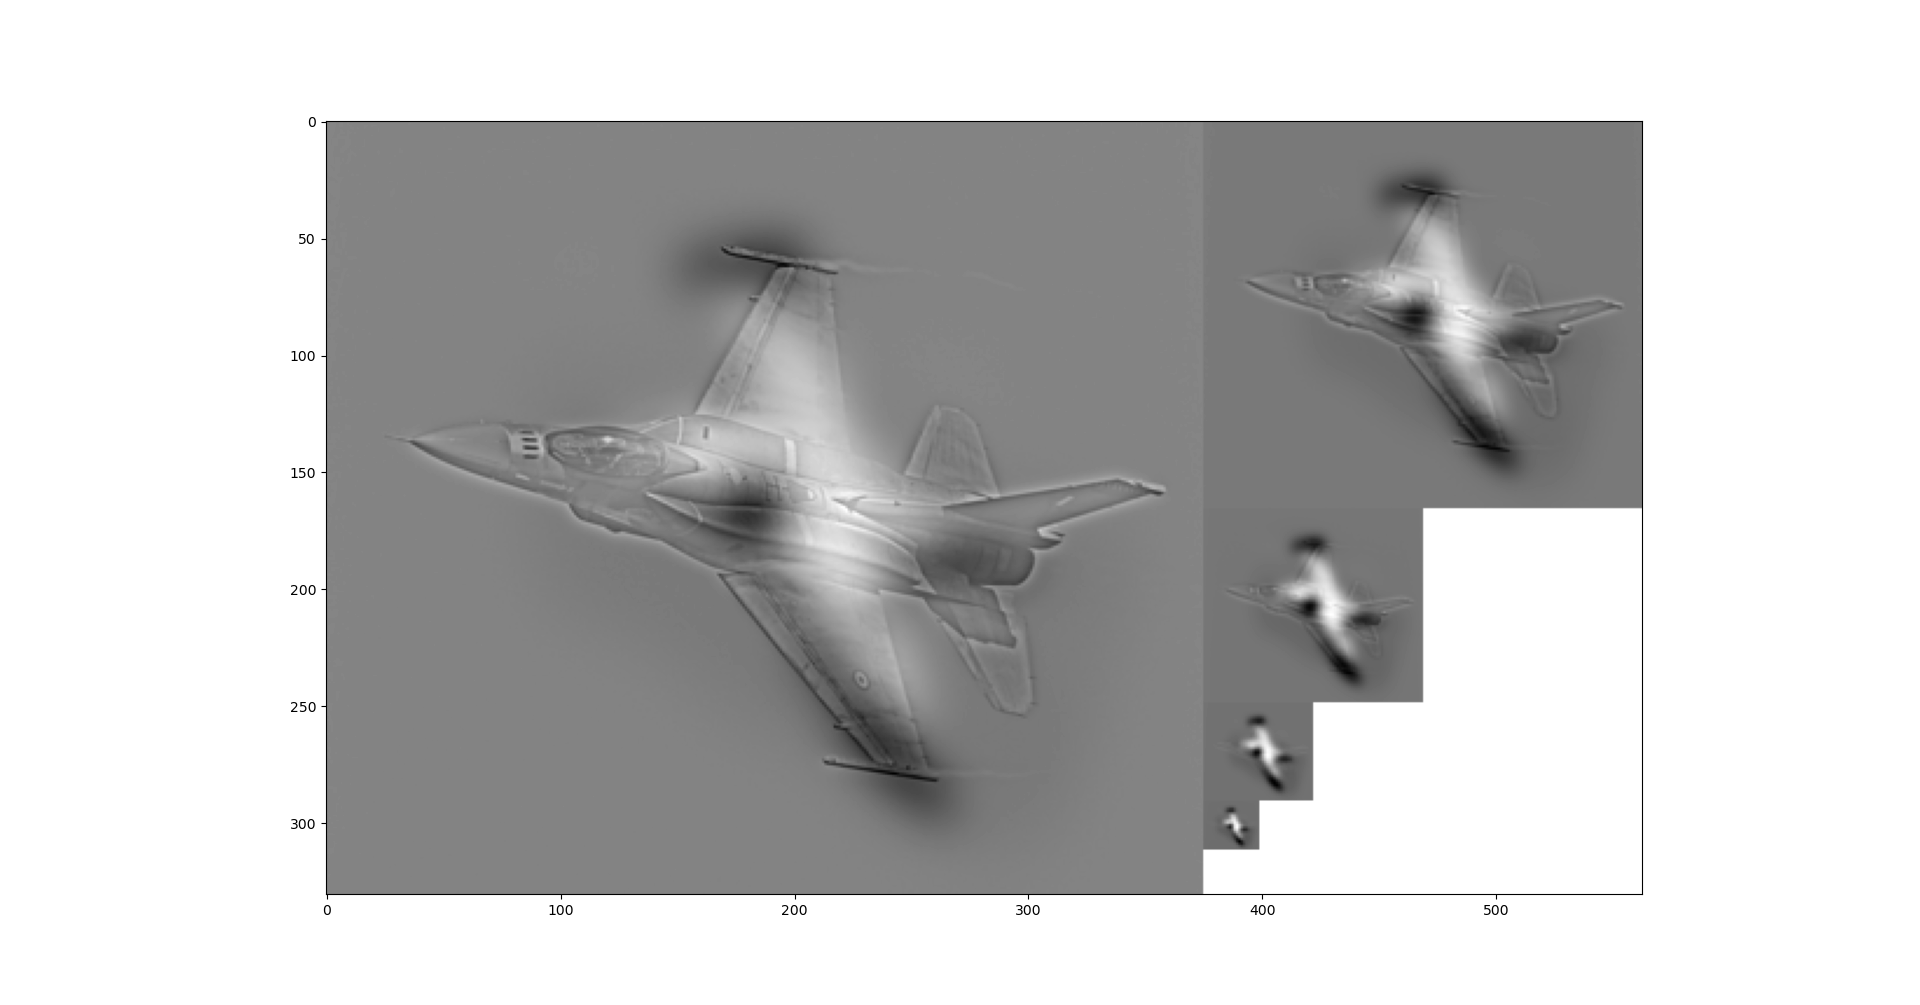
\includegraphics[width=\textwidth]{hibridas/PA-P.png}
 		 \caption{Pirámide de la imágen hibrida de un avión y un pájaro.}
  		\label{fig:ej2al}

\end{figure}

\begin{figure}[H]
  \centering
      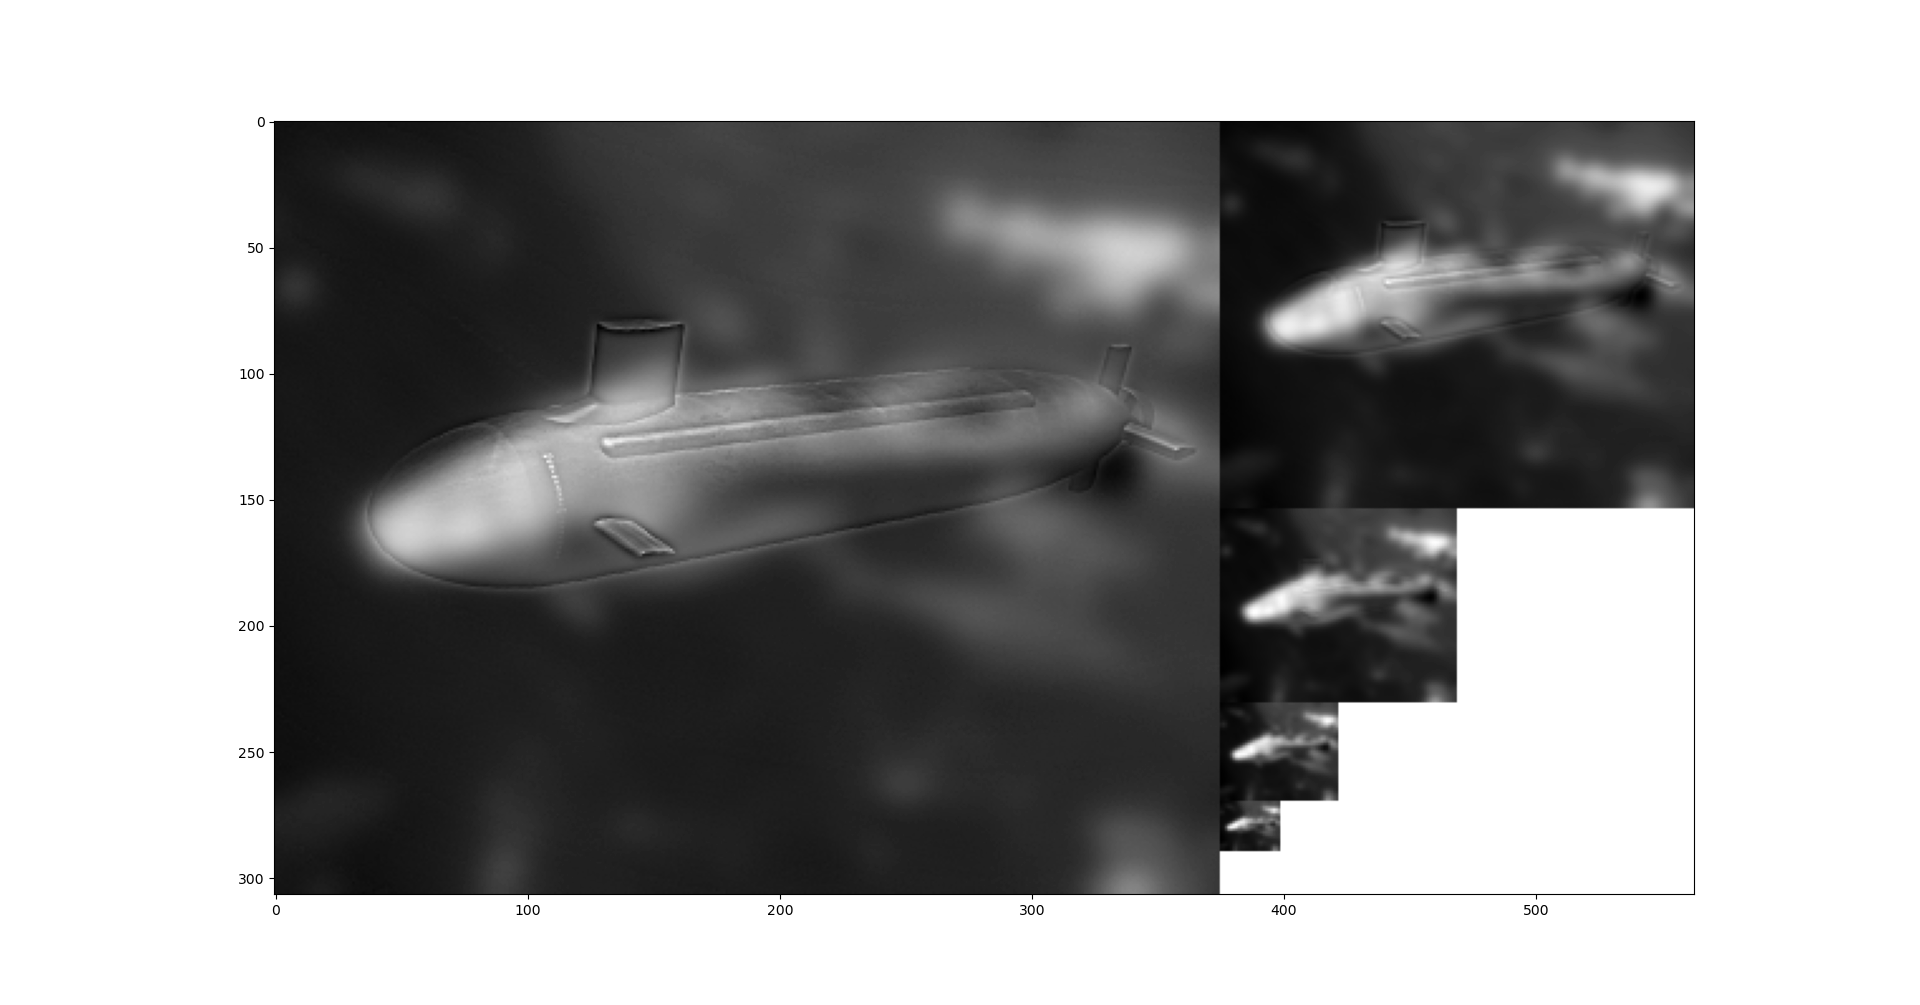
\includegraphics[width=\textwidth]{hibridas/PP-S.png}
 		 \caption{Pirámide de la imágen hibrida de un pez y un submarino.}
  		\label{fig:ej2al}

\end{figure}

Vemos como gracias a la pirámide gaussiana las diferencias entre observarla de cerca y de lejos es más clara.

Aun así vemos que en las imágenes híbridas se sigue observando cierta sombra de la imagen que no deberíamos ver de cerca, pero como comentan en el paper en el que nos hemos basado, esas sombras son las que nos permiten en la distancia reconocer la imagen de bajas frecuencias.

Es importante mencionar que estas imágenes híbridas se han podido construir ya que la posición de los objetos o personas que conforman la imagen híbrida es la misma.


\newpage

\section{Ejercicio bonus: Imágenes híbridas a color}

En este ejercicio bonus se nos pide hacer lo mismo que en el ejercicio 3 sin embargo con imágenes a color, y añadiendo una pareja de imágenes propia.

De cara a realizar las imágenes híbridas a color simplemente he modificado la función \texttt{aplicar\_convolución} para que tenga en cuenta si la imagen es monobanda o tribanda, de forma que aplique la convolución a todas las bandas. También he modificado la función \texttt{apilar\_piramide} para que tenga en cuenta las formas correctas para apilar las imágenes, pero esa función es simplemente para visualizar el resultado y no en un objetivo del ejercicio como tal, así que no entraré en detalle en esta memoria.

\subsection{Imágenes dadas}

Tras esta modificación obtenemos las siguientes imágenes híbridas:


\begin{figure}[H]
  \centering
      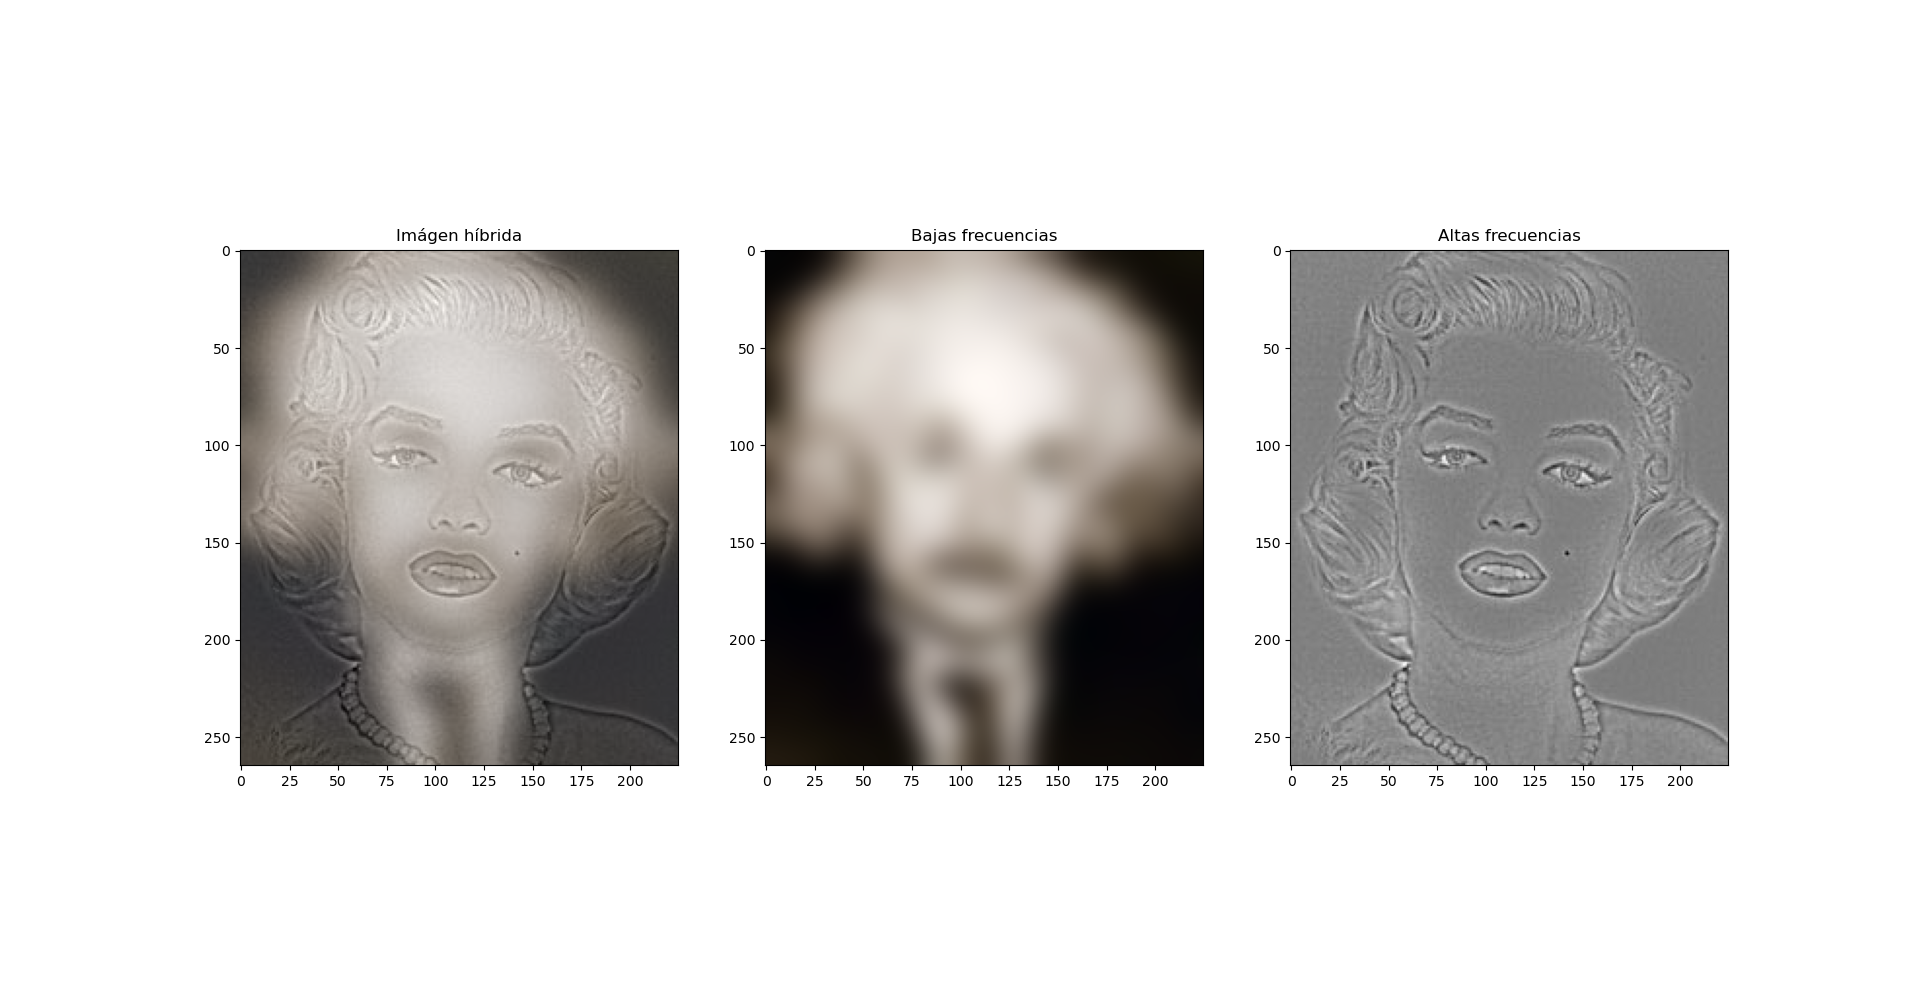
\includegraphics[width=\textwidth]{hibridas_color/E-M.png}
 		 \caption{Imágen hibrida de Eintein con Marylin.}
  		\label{fig:ej2al}

\end{figure}


\begin{figure}[H]
  \centering
      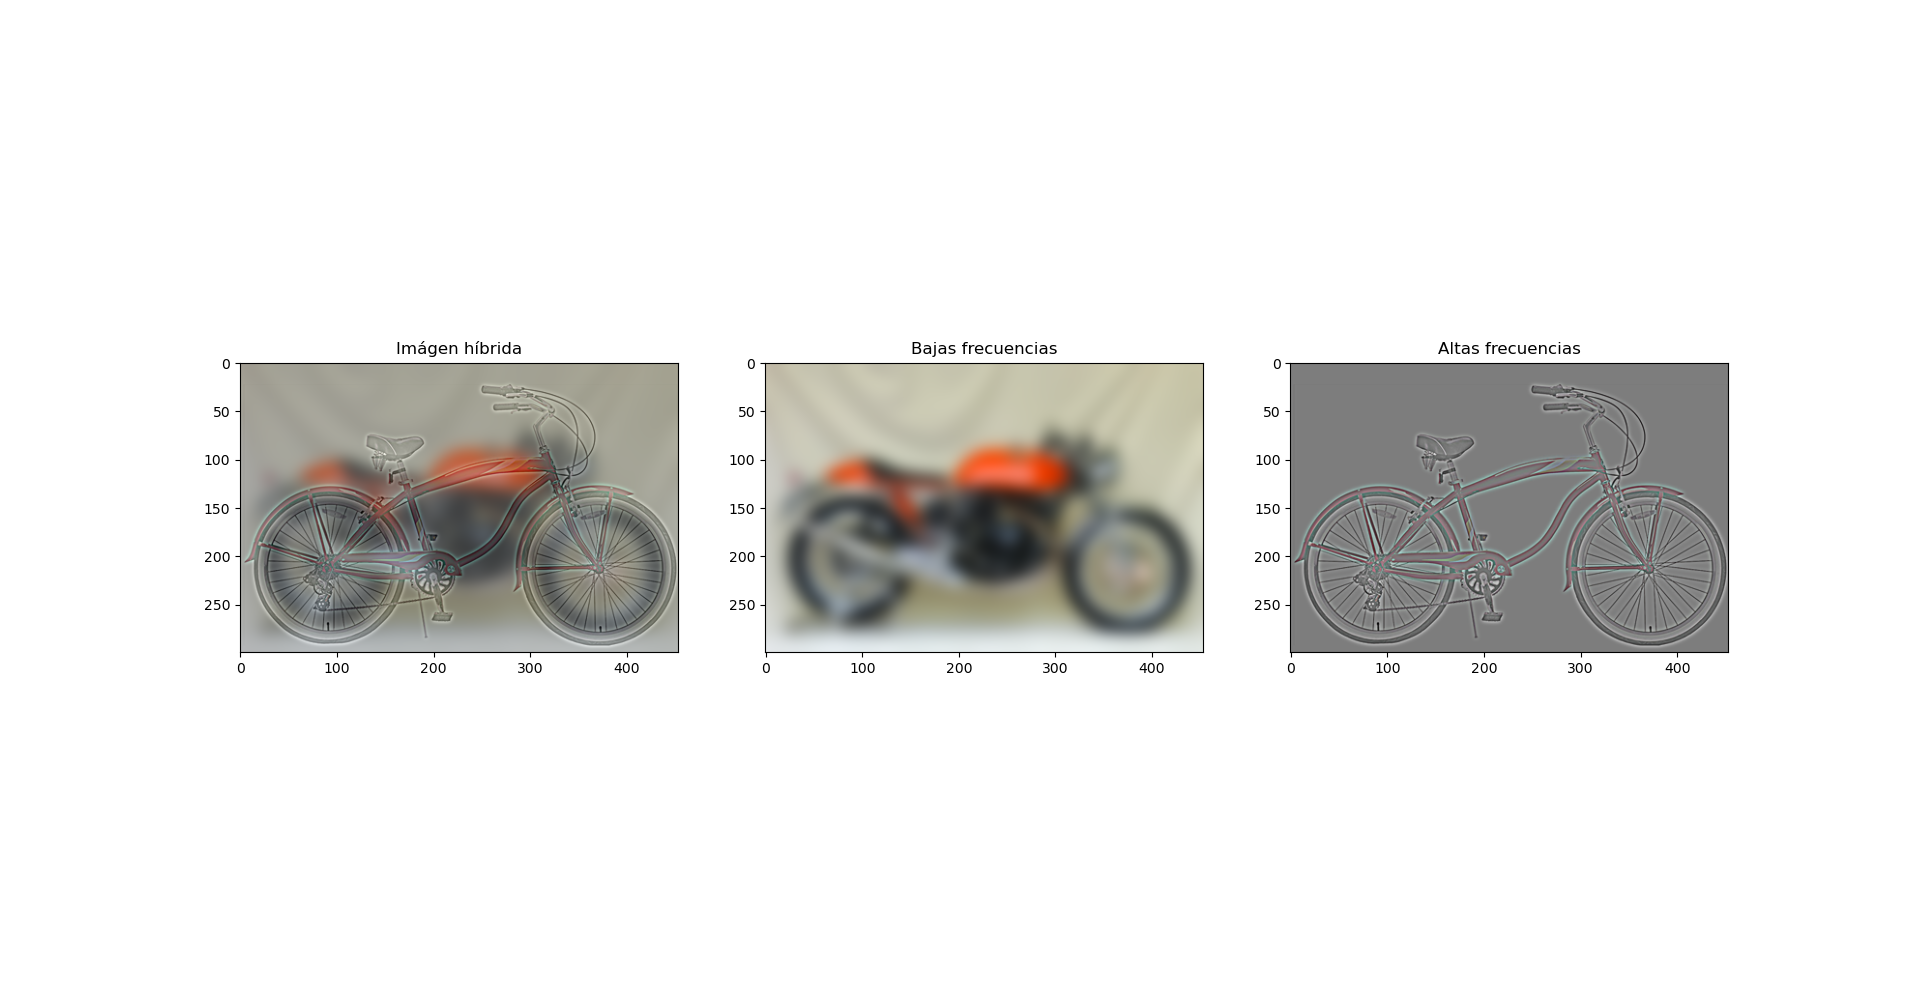
\includegraphics[width=\textwidth]{hibridas_color/B-M.png}
 		 \caption{Imágen hibrida de una bicicleta con una motocicleta.}
  		\label{fig:ej2al}

\end{figure}


\begin{figure}[H]
  \centering
      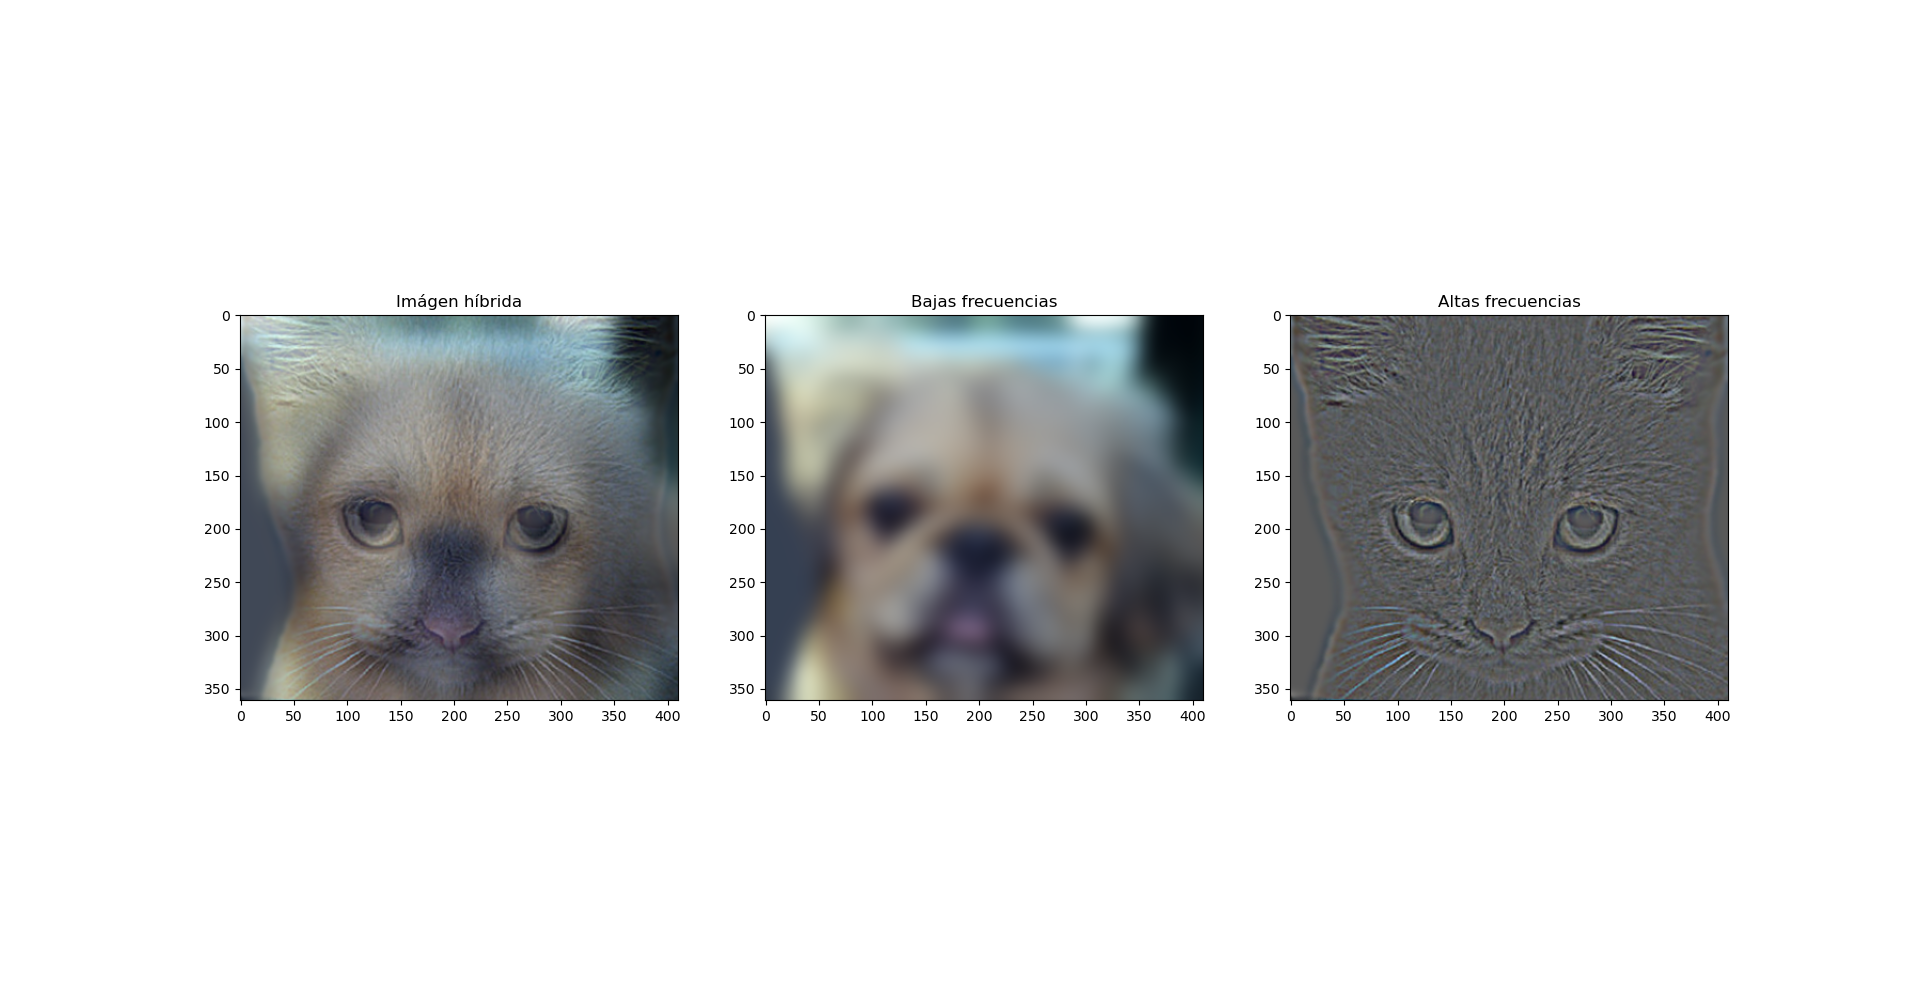
\includegraphics[width=\textwidth]{hibridas_color/G-P.png}
 		 \caption{Imágen hibrida de un gato y un perro.}
  		\label{fig:ej2al}

\end{figure}


\begin{figure}[H]
  \centering
      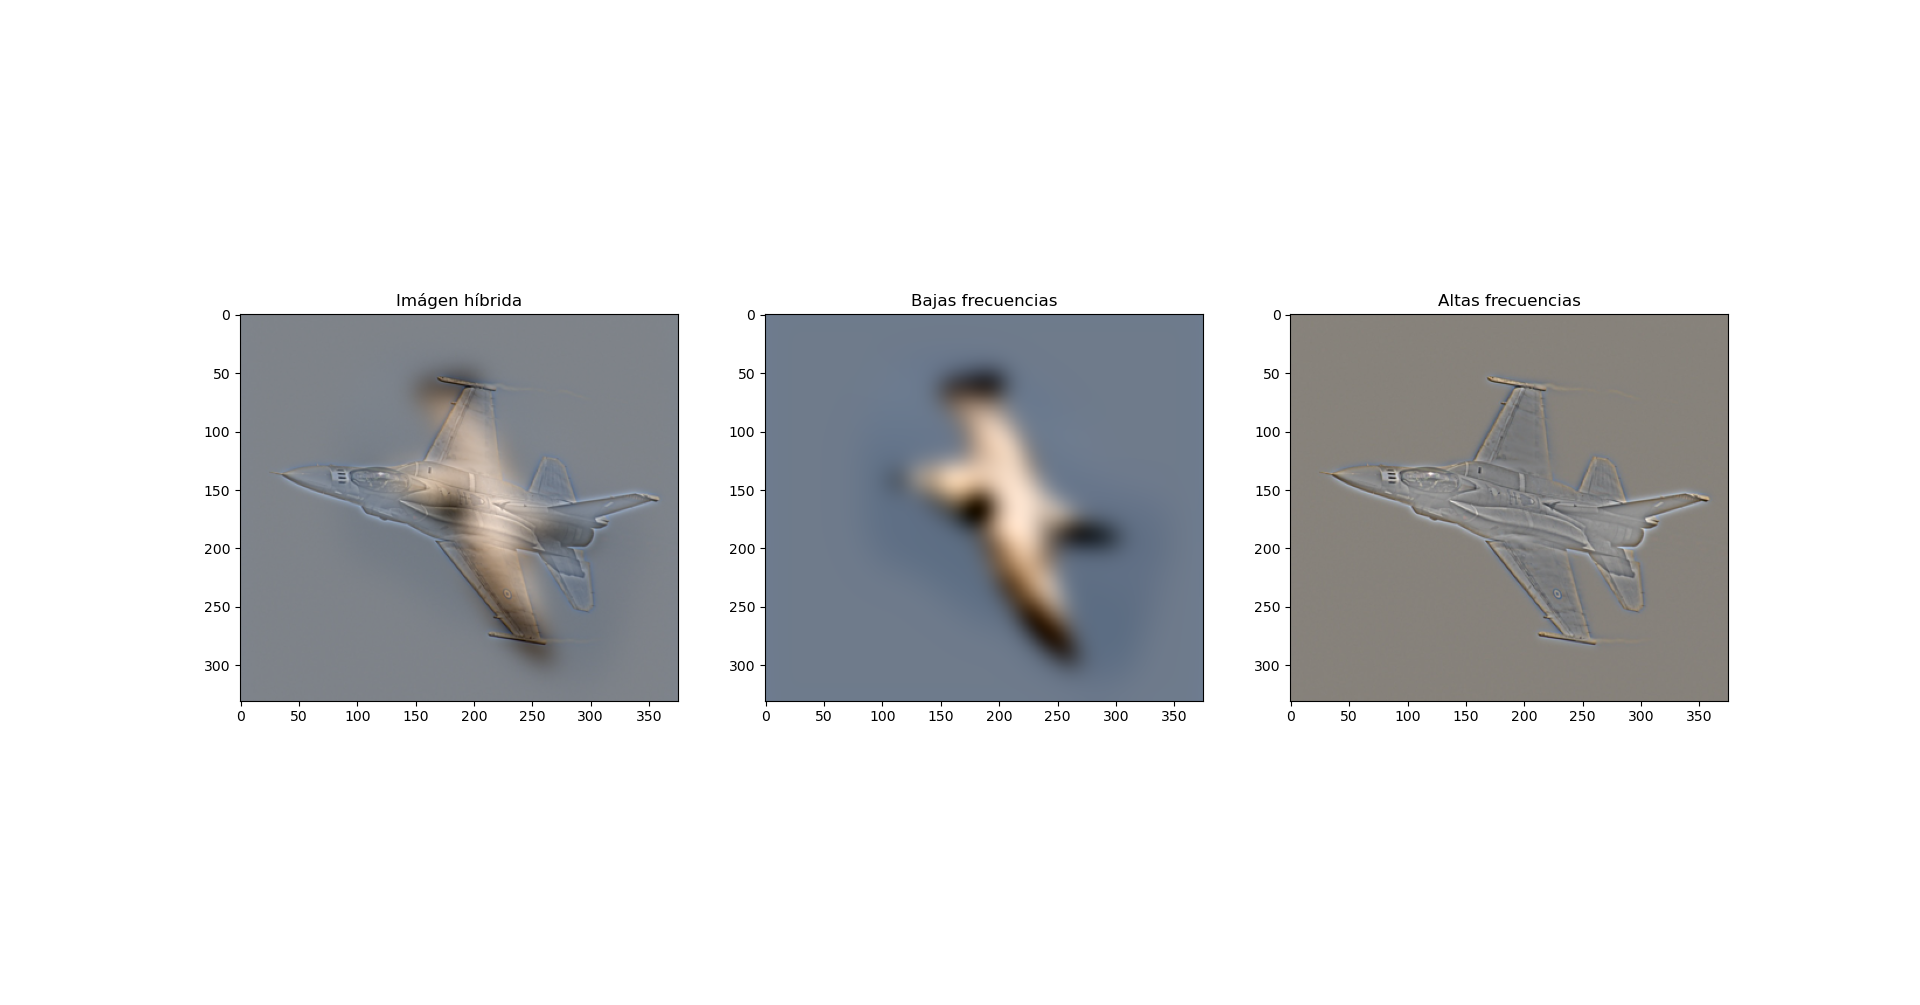
\includegraphics[width=\textwidth]{hibridas_color/A-P.png}
 		 \caption{Imágen hibrida de un avión y un pájaro.}
  		\label{fig:ej2al}

\end{figure}

\begin{figure}[H]
  \centering
      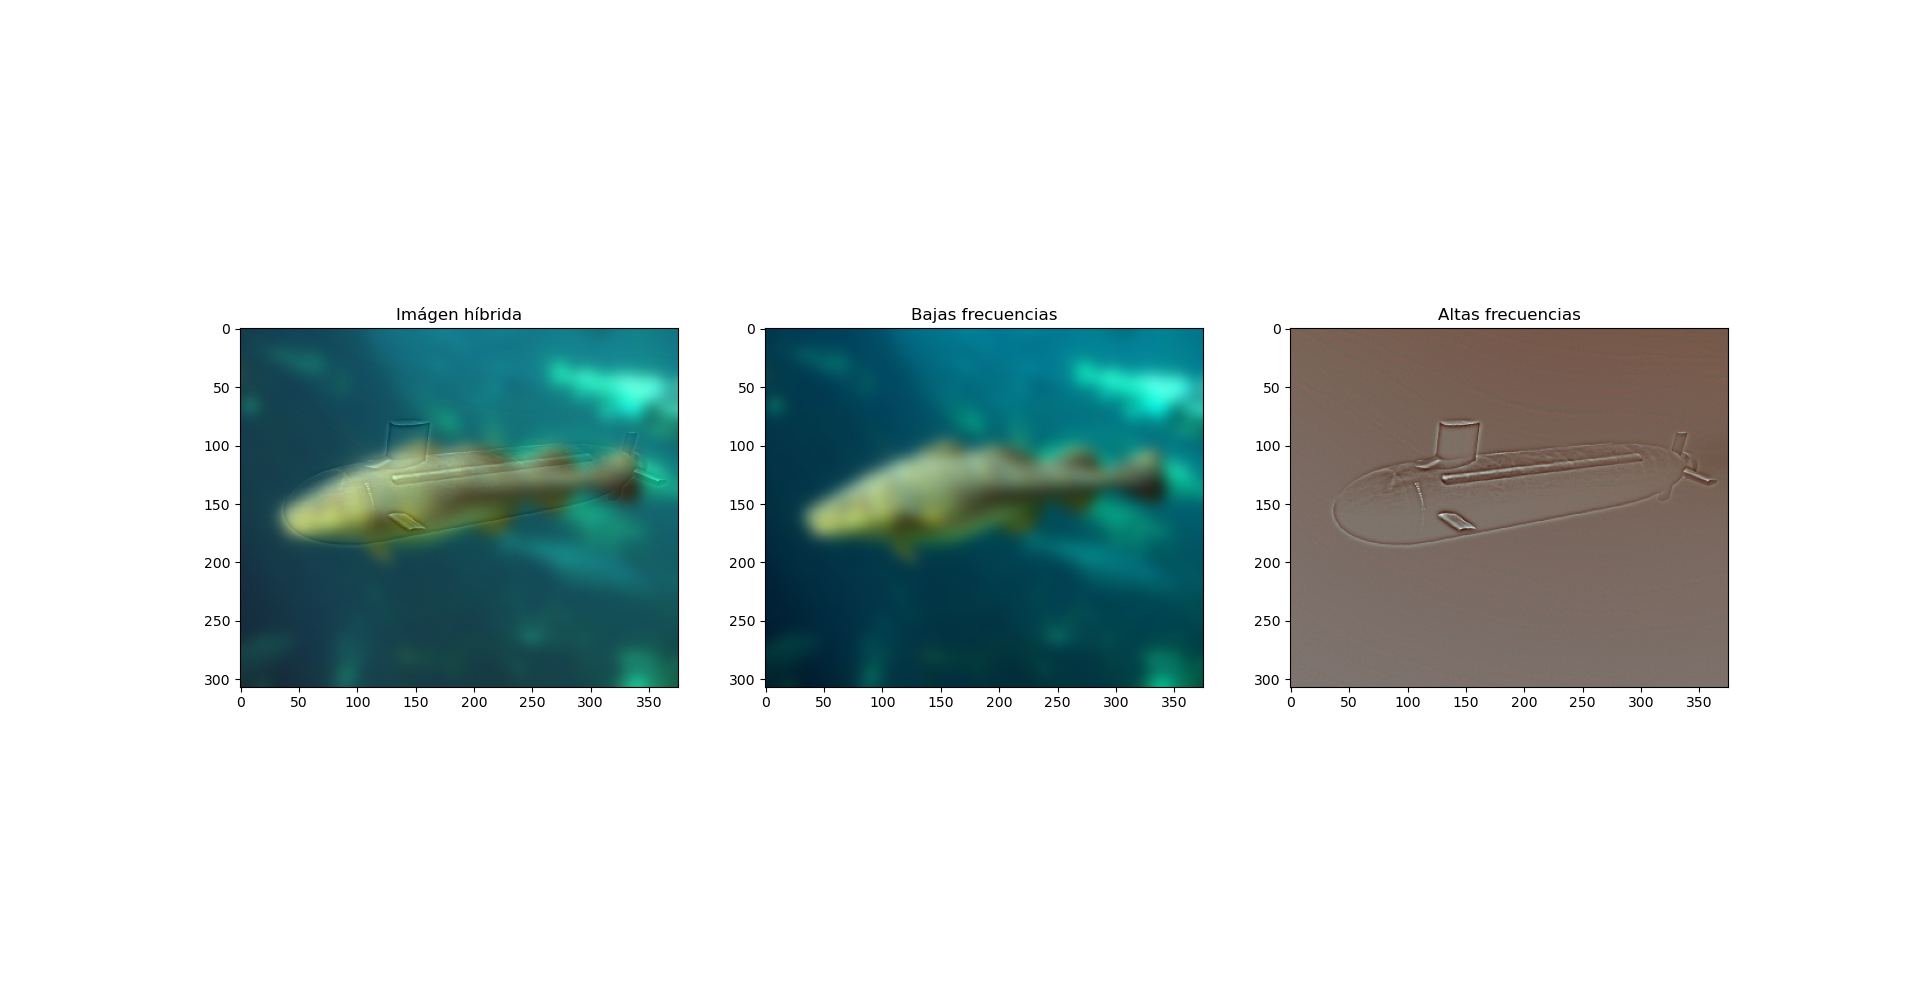
\includegraphics[width=\textwidth]{hibridas_color/P-S.png}
 		 \caption{Imágen hibrida de un pez y un submarino.}
  		\label{fig:ej2al}

\end{figure}


De cara a que la distinción sea más clara, como nos pide el ejercicio, mostraré la pirámide gaussiana obtenida de las imágenes hibridas utilizando la función desarrollada en el ejercicio 2:



\begin{figure}[H]
  \centering
      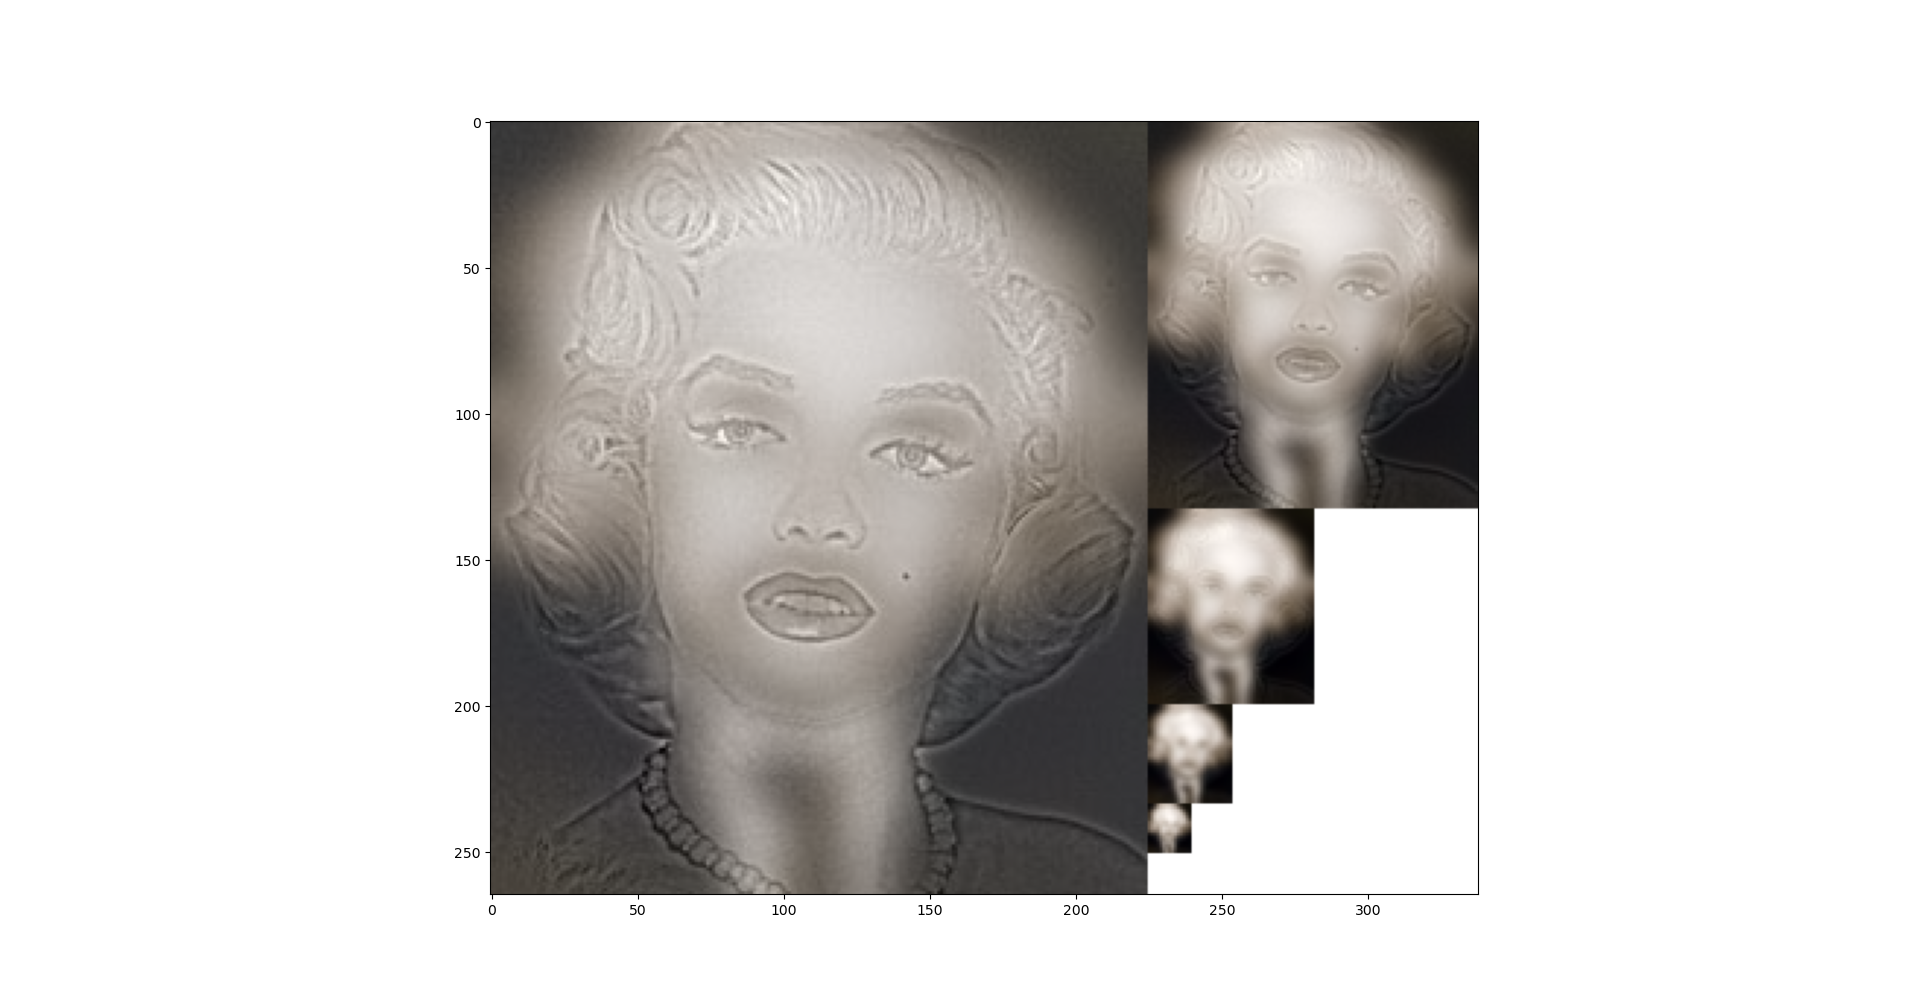
\includegraphics[width=\textwidth]{hibridas_color/PE-M.png}
 		 \caption{Pirámide gaussiana de la imágen hibrida de Eintein con Marylin.}
  		\label{fig:ej2al}

\end{figure}


\begin{figure}[H]
  \centering
      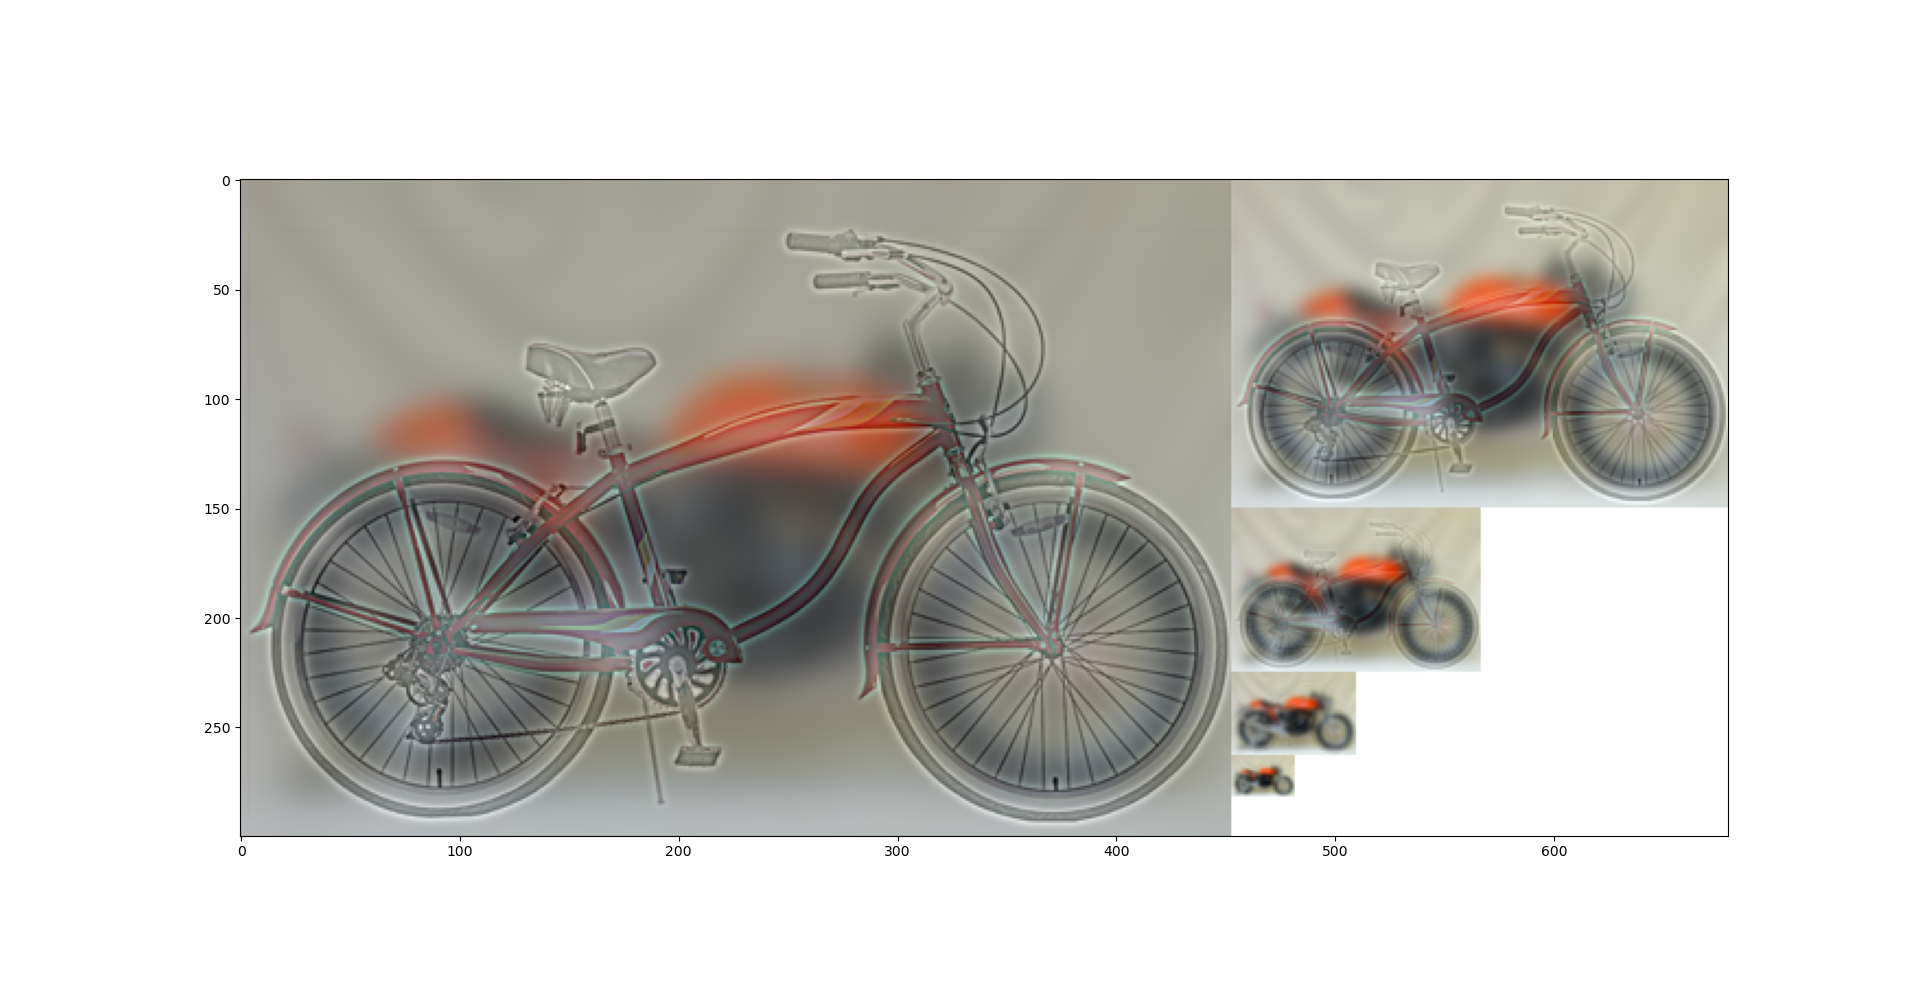
\includegraphics[width=\textwidth]{hibridas_color/PB-M.png}
 		 \caption{Pirámide gaussiana de la imágen hibrida de una bicicleta con una motocicleta.}
  		\label{fig:ej2al}

\end{figure}


\begin{figure}[H]
  \centering
      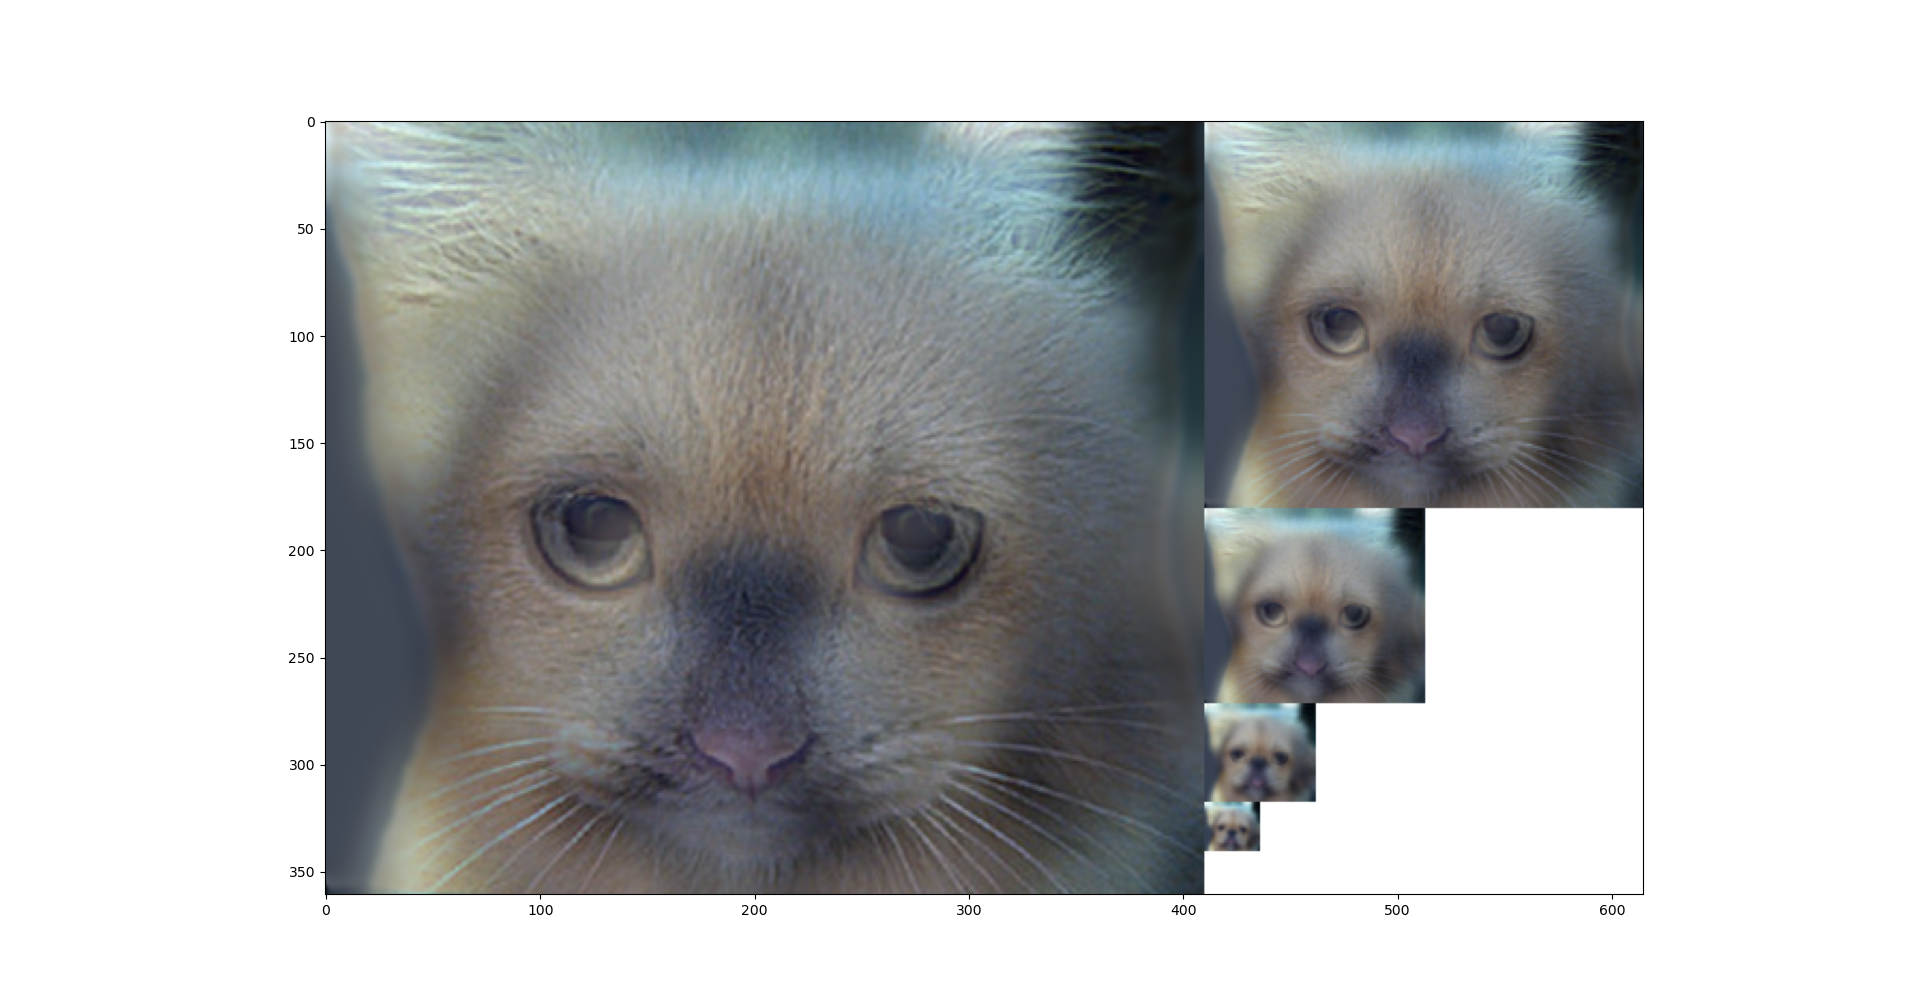
\includegraphics[width=\textwidth]{hibridas_color/PG-P.png}
 		 \caption{Pirámide gaussiana de la imágen hibrida de un gato y un perro.}
  		\label{fig:ej2al}

\end{figure}


\begin{figure}[H]
  \centering
      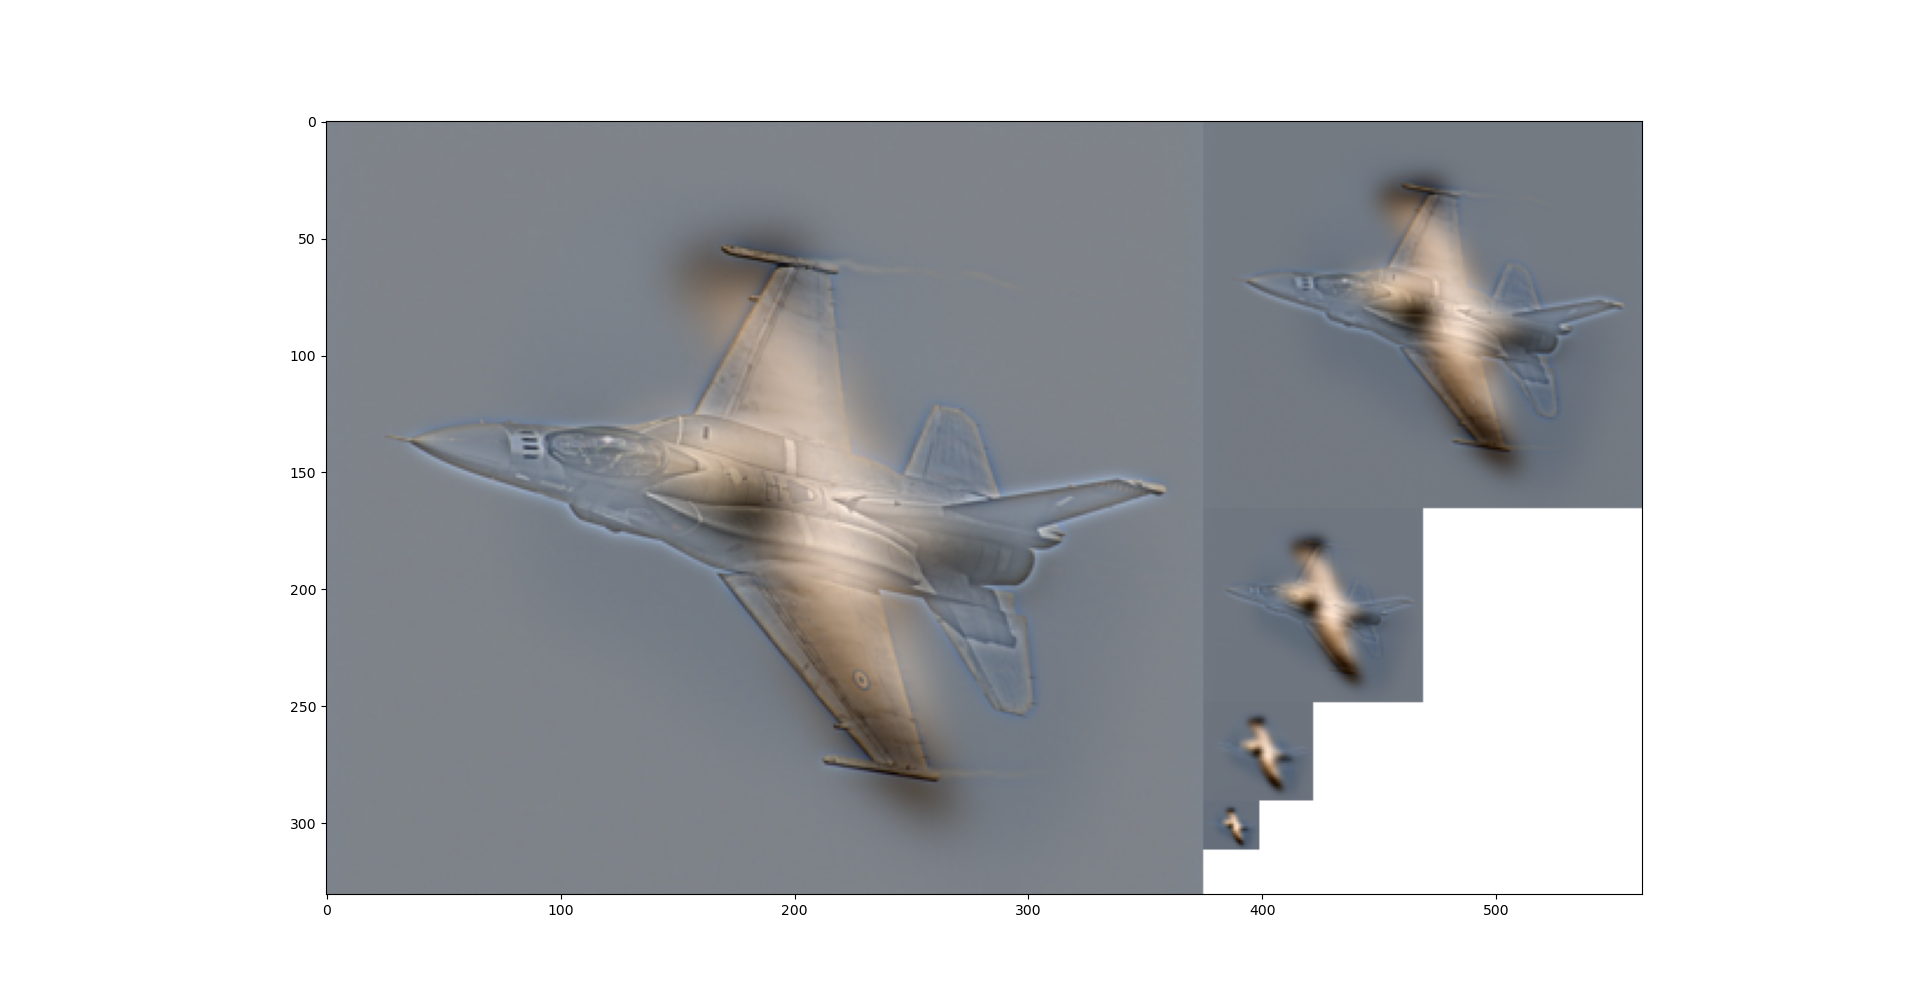
\includegraphics[width=\textwidth]{hibridas_color/PA-P.png}
 		 \caption{Pirámide gaussiana de la imágen hibrida de un avión y un pájaro.}
  		\label{fig:ej2al}

\end{figure}

\begin{figure}[H]
  \centering
      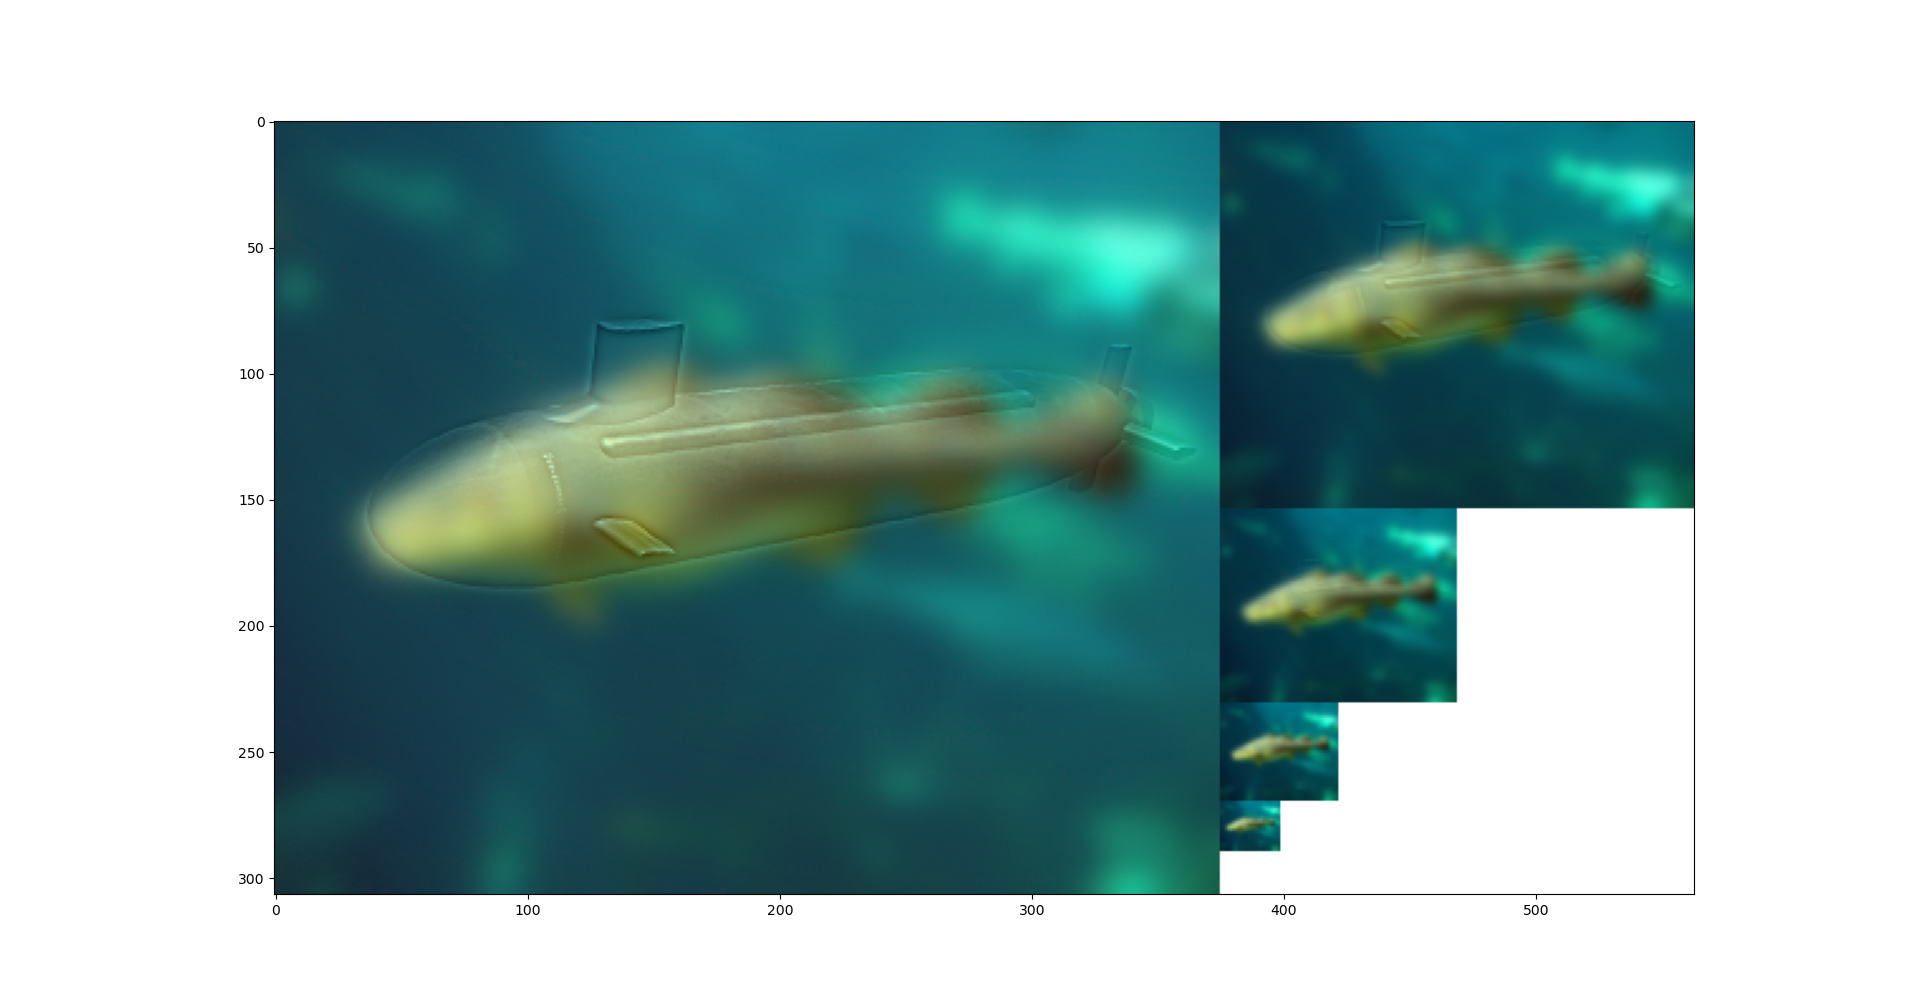
\includegraphics[width=\textwidth]{hibridas_color/PP-S.png}
 		 \caption{Pirámide gaussiana de la imágen hibrida de un pez y un submarino.}
  		\label{fig:ej2al}

\end{figure}

Vemos como el resultado de estas imágenes no es tan bueno, ya que las sombras que nos permitian ver las imágenes de bajas frecuencias, al estar a color, contaminan más la imagen híbrida final, por lo que hay que aumentar la distancia para distinguir una imagen de otra, aun así somos capaces de obtener un buen resultado.


\newpage


\subsection{Pareja de imágenes propia}

Para las imágenes propias he escogido las siguientes imágenes:

\begin{figure}[H]
  \centering
	\begin{subfigure}[t]{0.4\textwidth}
		\centering
      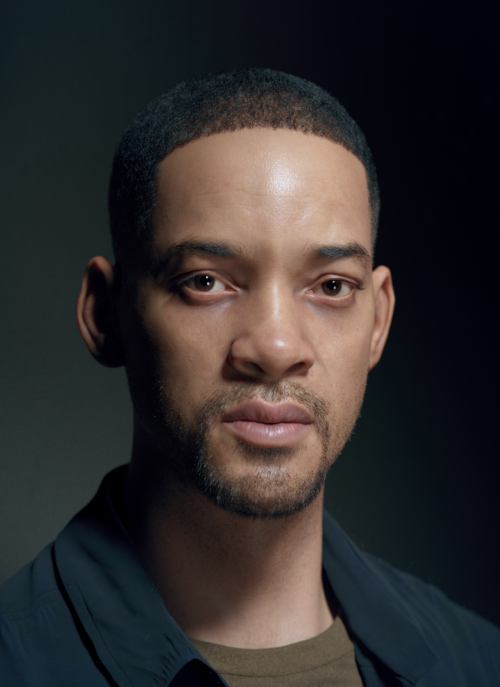
\includegraphics[scale = 1]{hibridas_color/will_smith.png}
 		 \caption{Will Smith.}
	\end{subfigure}
	\hspace{1cm}
	\begin{subfigure}[t]{0.4\textwidth}
		\centering
      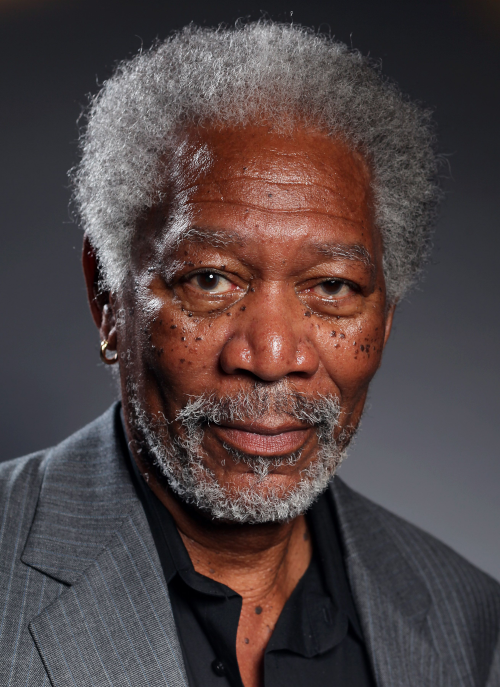
\includegraphics[scale = 1]{hibridas_color/morgan_freeman.png}
 		 \caption{Morgan Freeman.}
	\end{subfigure}
	\caption{Imágenes escogidas para realizar el bonus.}

  	\label{fig:bonus}
\end{figure}

He escogido estas imágenes ya que se tratan de imágenes con fondos similares, ambas personas aparecen en la misma posición, con la posición de los rasgos de la cara coincidentes y ambos tienen el mismo tono de piel, por lo que no se crearían sombras extrañas al hacer la imagen híbrida. El resultado es el siguiente:


\begin{figure}[H]
  \centering
      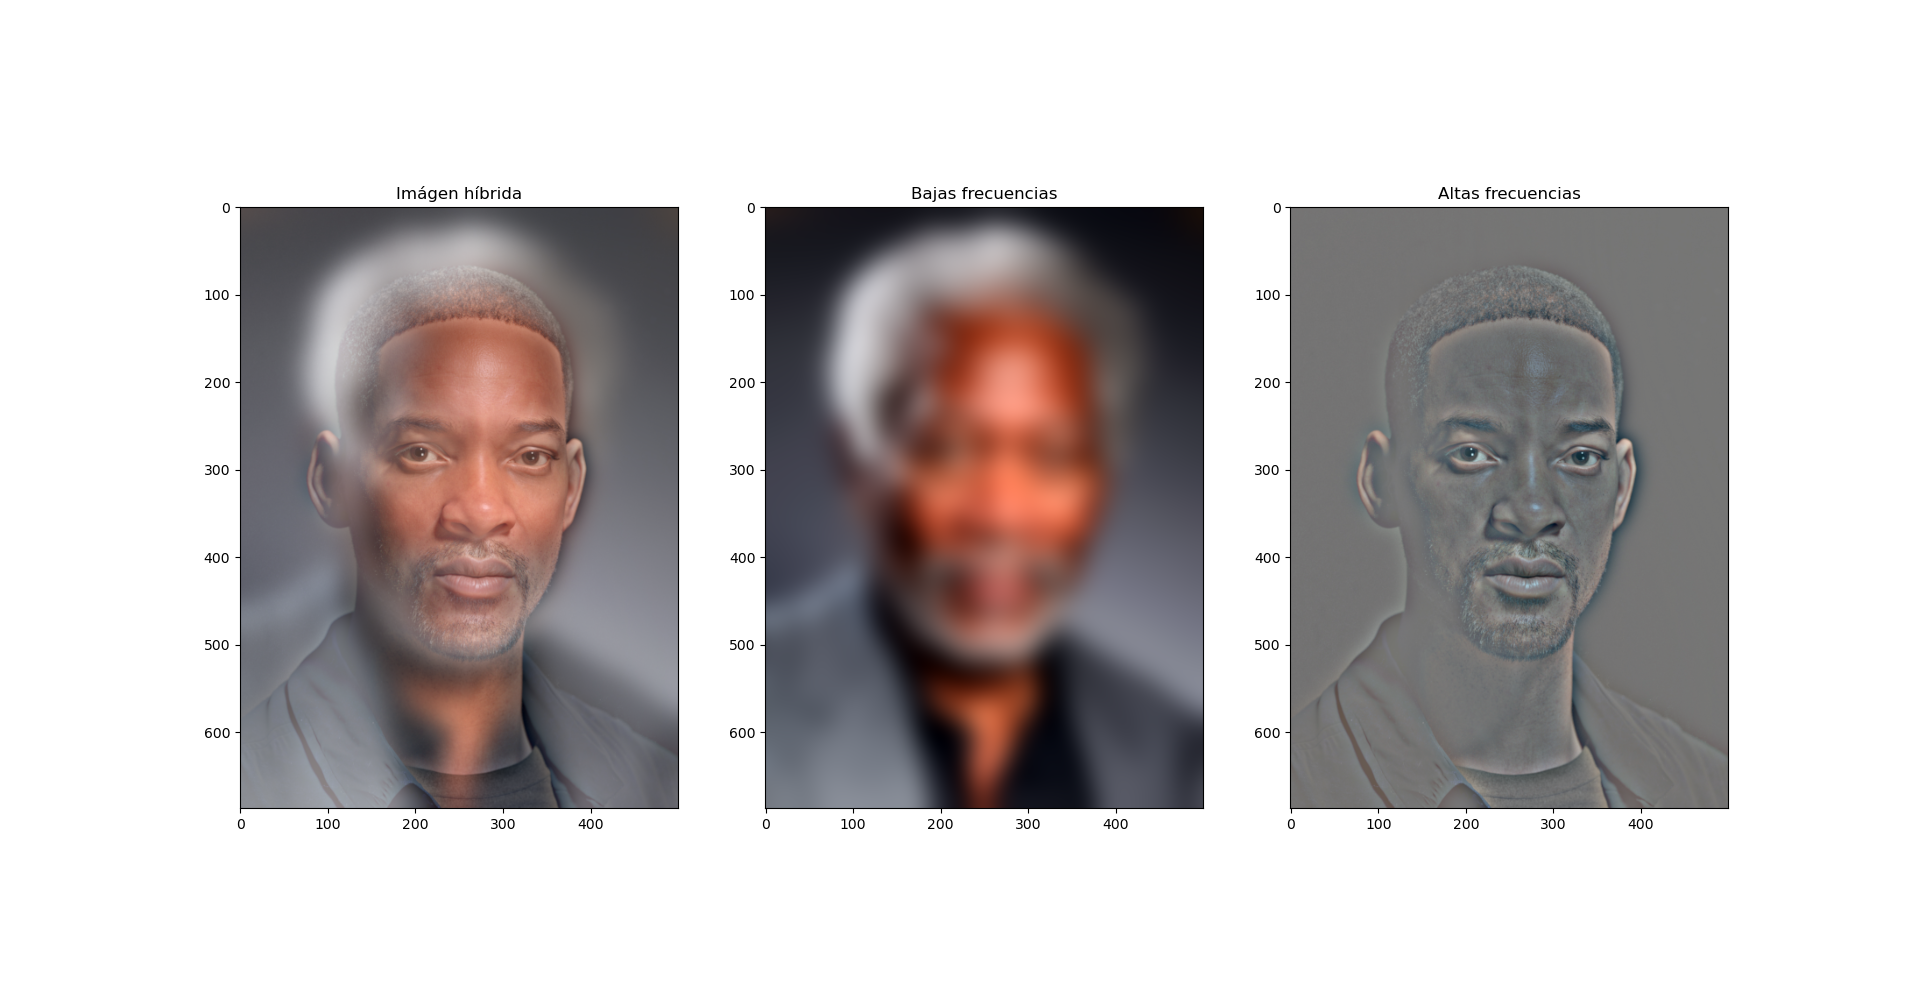
\includegraphics[width=\textwidth]{hibridas_color/W-F.png}
 		 \caption{Imágen hibrida de Will Smith y Morgan Freeman.}
  		\label{fig:ej2al}

\end{figure}

\begin{figure}[H]
  \centering
      \includegraphics[width=\textwidth]{hibridas_color/PW-F.png}
 		 \caption{Pirámide gaussiana de la imágen hibrida de Will Smith y Morgan Freeman.}
  		\label{fig:ej2al}

\end{figure}

\newpage

\section{Referencias, material y documentación usada}


\begin{thebibliography}{9}

\bibitem{separabilidad_2D}
	Prueba de separabilidad para las convoluciones 2D.

	\url{https://www.songho.ca/dsp/convolution/convolution2d_separable.html}

\bibitem{getDerivKernelsCV}
	getDerivKernels - Documentación oficial de OpenCV.

	\url{https://docs.opencv.org/4.4.0/d4/d86/group__imgproc__filter.html#ga6d6c23f7bd3f5836c31cfae994fc4aea}



\bibitem{img_hibridas}

	A. Oliva, A. Torralba, P.G. Schyns(2006). Hybrid Images. ACM Transactions onGraphics.

	\url{http://olivalab.mit.edu/hybridimage.htm}


\end{thebibliography}

\end{document}
